
%-----------------------------------------------------------------------------------------------------------------------------------------
% PACKAGES
%Document Class starts every LaTeX document.  In this case, we're declaring the document class to be a book.  Changing "oneside" to "twoside" changes where the page numbers and headers and such get placed.
\documentclass[12pt,oneside]{book}

%These are the packages I used.  There's a description of (most of) them below (that Arthur wrote):
\usepackage{fancyhdr, geometry, graphicx, epstopdf, lscape, setspace, amssymb, amsmath, wasysym,moreverb, natbib, titlesec, longtable, multirow, multicol, alltt,here, indentfirst,ifthen,xfrac,relsize,rotating}

\usepackage[small,bf]{caption}
\geometry{letterpaper}



%The "raggedbottom" command allows LaTeX to take some liberty with where the text on a page ends. This saved me some weird formatting problems I was having.
 \raggedbottom
 

%set the pagestyle:
\fancypagestyle{plain}{
\fancyhf{} % clear all header and footer fields, we will re-format them later

%Some formatting stuff:
\newcommand*\rfrac[2]{{}^{#1}\!/_{#2}}
\renewcommand{\headrulewidth}{0pt}
\renewcommand{\footrulewidth}{0pt}}
\newcommand{\upperRomannumeral}[1]{\uppercase\expandafter{\romannumeral#1}}
\newcommand{\lowerromannumeral}[1]{\romannumeral#1\relax}

%journal definitions
\newcommand{\aap}{{\it A\&A}}
\newcommand{\aaps}{{\it A\&AS}}
\newcommand{\aj}{{\it AJ}}
\newcommand{\apj}{{\it ApJ}}
\newcommand{\apjl}{{\it ApJL}} 
\newcommand{\apjs}{{\it ApJS}}
\newcommand{\araa}{{\it ARA\&A}}
\newcommand{\iaucirc}{{\it IAU Circular}}
\newcommand{\mnras}{{\it MNRAS}} 
\newcommand{\nat}{{\it Nature}}
\newcommand{\pasj}{{\it PASJ}}
\newcommand{\pasp}{{\it PASP}}
\newcommand{\ssr}{{\it SSRv}}
\newcommand{\sciam}{{\it Scientific American}}
\newcommand{\jgr}{{\it JGR}}
\newcommand{\grl}{{\it GRL}}
\newcommand{\icarus}{{\it ICAR}}
\newcommand{\na}{{\it NA}}
\newcommand{\actaa}{{\it ACA}}
\newcommand{\apss}{{\it Ap\&SS}}




%	NECESSARY PACKAopticallasdfGES
%	fancyhdr enables use of fancy pagestyle
%	geometry defines page layout
%	graphicX allows for inclusion of graphics and page scaling and rotation
%	epstopdf allows the conversion of eps files to pdf and is required for figures
%	caption allows the captioning of figures
%	lscape allows for the creation of landscape pages-- important for large tables
%	setspace allows for doublespacing
%	natbib allows for the citations and Bibtex
%	titlesec allows for the definition of title layouts

%	OPTIONAL PACKAGES
%	aastex is only useful for article submission
%	revsymb is for physics symbols
%	amssymb is for math symbols
%	amsmath is for math formatting for things like matrices
%	parskip (\usepackage[parfill]{parskip})  allows paragraphs to begin with empty line
%	mathrsfs is required for \mathscr, the best Lagrangian and FT font
%	here makes !h force graph here and !t force the graph at the top of the page
%	wrapfig allows the wrapping of figures
%	fontspec allows the specification of fonts
%	color allows for the specification of the color of fonts
%	eso-pic allows the addition of watermarks such as a draft date


%-----------------------------------------------------------------------------------------------------------------------------------------
% RULES

%This has something to do with headers and margins and stuff:
\DeclareGraphicsRule{.tif}{png}{.png}{`convert #1 `dirname #1`/`basename #1 .tif`.png}
\textwidth 5.750in \textheight=8.50in \headheight 0.0625in \topmargin 0.0in % book strict

%==============================================================================
% Uncomment below for one sided printing (margins the same on even and odd pages)
\oddsidemargin 0.500in \evensidemargin 0.500in

% Uncomment below for two sided printing (margins different on even and odd pages)
%\oddsidemargin 0.563in \evensidemargin 0.2500in

%This sets how we want the formatting of chapter titles to look (bold face and Huge):
\titleformat{\chapter}{\bf\Huge}
{Chapter \thechapter}{-4.4em}{\\}
\titlespacing*{\chapter}{0pt}{-.57in}{*3}

%This formats the section headings:
\titleformat{\section}{\bf\Large}
{\thesection}{1em}{}
\titlespacing*{\section}{0pt}{*2}{*2}

%Let's double-space the document:
\doublespacing

%And our citation style will be aa (astronomy style):
\citestyle{aa}

%-----------------------------------------------------------------------------------------------------------------------------------------
% DOCUMENT/ TITLE PAGE
%Now the document actually begins:
\begin{document}

%This states that this is the stuff that comes before the real text:
\frontmatter

%Here goes the title page:
\pagestyle{empty}
\begin{titlepage}
\begin{center}
\rule{5.75in}{1pt} \\
\vspace*{-0.125in}
{\large \doublespacing Wesleyan University} \hfill {\large \doublespacing The Honors College}
\rule[0.2in]{5.75in}{1pt} \\
\vspace*{0.8in}
{\LARGE \singlespacing \bf The Mysterious Case \\ of 49 Ceti: \\A Gas-Rich Debris Disk\\ And Its Implications\\For Planet Formation} \\
\vspace*{0.05in}
\vspace*{0.10in}
{\large \vspace*{0.20in}  \singlespacing by \vspace*{.2in}
\\Jesse Lieman-Sifry \\ Class of 2015\\}
\vspace*{0.25in}
\vspace*{0.8in}
{\large \singlespacing A thesis submitted to the\\ faculty of Wesleyan University\\ in partial fulfillment of the requirements for the \\ Degree of Bachelor of Arts\\ with Departmental Honors in Astronomy\\ \vspace*{-0.15in} }
\vspace*{.25in}
\rule{5.75in}{1pt} \\
\vspace*{-0.125in}
{\large \doublespacing Middletown, Connecticut \hfill April, 2015}
\rule[0.2in]{5.75in}{1pt} \\
\end{center}
\end{titlepage}


%-----------------------------------------------------------------------------------------------------------------------------------------
% ABSTRACT/ ACKNOWLEDGEMENTS
%After the title page, comes anything else you want before the Table of Contents.  Note that the Epigraph and acknowledgements are in their own files.  The \include command inserts the external files into the final document.

\pagestyle{empty}
%\pagestyle{plain}

\mbox{}
\vspace{.75in}
\hrule

\vspace{2in}


%\begin{minipage}[c]{4in}
\begin{centering}
	\hspace{.25in} 
	\parbox{5in}{
		\noindent 
		\textit{We are just an advanced breed of monkeys on a minor planet of a very average star. But we can understand the Universe. That makes us something very special.}
		\vspace{3pt}

		\begin{flushright}
			{\sc {--Stephen Hawking}}\\
		%	{\textit{The Hitchhiker's Guide to the Galaxy}}
		\end{flushright}
	}
\end{centering}
\vspace{2.25in}
\hrule
\vfill



%\flushleft















\textwidth 5.750in \textheight=8.50in \headheight 0.0625in \topmargin 0.0in % book strict

\chapter{Acknowledgements}

I would like to thank Meredith Hughes for being an amazing mentor through the process of teaching me to do advanced research, all the way from the crash course in radio astronomy at the beginning of my Junior year through this thesis. I'm blessed to have worked with such a dedicated advisor who cares so much about the learning process for each and every student. Going to Hawaii to observe at the SMA and Seattle for AAS were unforgettable experiences that not many undergraduates have, but those are really just cherries on top of the incredible sundae of knowledge, experience, and wisdom that you've passed on to me. 

Thanks to Seth Redfield for selling me on the astronomy program here at Wesleyan and getting me involved with the 24$''$ observing program. I may never live down getting flung from my chair as the monkey in an angular momentum demonstration he put me up to, but at least I'm better at ultimate frisbee. 

Thanks to Kevin Flaherty, for helping me out with everything from cluster computing to statistical tests, and to Roy Kilgard, for the endless patience in helping me with computer issues and always being fun to stop by and talk to. Thanks to Angelo Ricarte for writing the foundation of the modeling code that I used in this thesis. 

To Mom and Dad, thanks for giving me multiplication problems before bed to help me fall asleep, even if you didn't always know the correct answer. I wouldn't be who I am today without your love and guidance. Mira, you're the best sister a little bro could ask for. 

To the basement crew, thanks for endless entertainment in times of drastic procrastination, playing darts, and letting me fly the baby drone around the library when that was our workspace without going crazy (RIP baby drone. Both a sorry and a damn you to the Fisk Telescope for breaking the last propellor). 

\titlespacing*{\chapter}{0pt}{*2}{*3}


%My title formatting changes after the frontmatter, because of how i formatted my acknowledgements:

\titleformat{\chapter}{\bf\Huge}
{Chapter \thechapter}{-4.4em}{\\}
\titlespacing*{\chapter}{0pt}{*2}{*3}

\titleformat{\section}{\bf\Large}
{\thesection}{1em}{}
\titlespacing*{\section}{0pt}{*2}{*2}


%-----------------------------------------------------------------------------------------------------------------------------------------
% CONTENTS/ RULES OF HEADERS
%LaTeX creates a table of contents for you automatically, but you may have to compile the document twice before it shows up properly:

\tableofcontents  \pagestyle{empty}

%You can also put in the following, if you wish:

%\listoffigures
%\listoftables \pagestyle{empty}


%Now we start the real part of the document:
\mainmatter


%-----------------------------------------------------------------------------------------------------------------------------------------
% HEADERS
%This took me forever to figure out properly, and you may want to change it.  There's also different thing you can do if you want doublesided printing.  Your final thesis, as published by the University, is one-sided.


\renewcommand{\chaptermark}[1]{ \markboth{\sc\thechapter.\ #1}{}}

\pagestyle{fancy}
\fancyhead{}
\fancyfoot{}

\fancyhead[L]{\leftmark}
\fancyhead[R]{\thepage}

%==============================================================================
%Number your pages!  
\pagenumbering{arabic}

%-----------------------------------------------------------------------------------------------------------------------------------------
% CHAPTERS
%Here's the actual thesis:  (note that file names CAN'T have spaces in them!)

\chapter{Introduction}

Circumstellar disks of gas and dust, left over from the processes of stellar formation, are cosmic nurseries for the growth of planets. In these young stellar systems, bodies ranging from small and rocky to massive and gaseous coalesce as gravitational, chemical, and viscous evolution transform gas-rich protoplanetary disks into tenuous, nearly gas-free debris disks over millions of years. While the direct detection of planets during this time is effectively impossible with our current technology, observations of rotational transitions of gas species, scattered light from micron-sized dust grains, and thermal emission from micron to millimeter-sized grains provide an indispensable tracer of the processes that shape these disks. Because the genesis of planets is directly tied to the morphology of the gas and dust, studying the anatomy of a variety of young disks is essential to understanding how worlds such as our own formed. 49 Ceti, at an estimated age of 40 million years, is just one puzzle piece of many, but its gas-rich debris disk provides important clues to deciphering the final stages of disk evolution. 

%49 Ceti is in the process of transitioning from a gas-rich disk to a tenuous, nearly gas-free debris disk, which makes it the perfect target to probe the processes by which the gas and dust dissipate.  

%Because the genesis of planets is directly tied to the morphology of the gas and dust and their development over time, observing the anatomy of nearby disks is helping us piece together the means by which planets form.  

%Characterizing the transitional phase from young, gas-rich protoplanetary disks to older, tenuous, and nearly gas-free debris disks is imperative for understanding how these planetary systems form. 

%Gas giants, such as Jupiter and Saturn, are thought to form from runaway accretion of gas onto a rocky core. However, in the 10 million years it takes the rocky core to form, most primordial gas has already disappeared. 
%Using CO as the tracer, observations have shown that the bulk of primordial gas dissipates within $\sim$ 10Myr, with less than a Jupiter mass generally remaining after only a few million years \citep{Zuck95}. Th
%and because we assume that the evolution of the gas is closely tied to that of the dust, 

%\section{Planet Formation Processes Dispersal of Gas and Dust}
\section{Planet Formation and The Evolution of Protoplanetary Disks to Debris Disks}

The collapse of giant clouds of molecular hydrogen leads directly to the formation of stars and their accompanying protoplanetary disks. As such, the mass of such a disk, which is generally on order 0.5$\%$ that of the star \citep{Andr13}, is dominated by primordial H$_{2}$. Although the dust contributes significantly less mass, a key characteristic is that it is optically thick in protoplanetary disks, but optically thin in debris disks \citep{Wyat14}. Surveys have found the median lifetime of dust disks is only a Myr \citep{Mama09} and that the bulk of primordial gas dissipates within 10\,Myr \citep{Zuck95}, putting a critical cutoff on the planet formation timeline for both rocky and gaseous planets. The ever-growing wealth of planets discovered around stars of all spectral types suggest that planetary systems are a common endpoint for the evolution of circumstellar material \citep{Howa13}. Thus, planet formation theories must show that the majority of disks can form gas planets within a few Myr, or that substantial amounts of gas persist beyond the dissipation of the optically thick dust disk. Recent statistical analyses suggest that at least $\sim$ 17$\%$ of stars host a Jupiter-mass planet (0.3-10M$_{Jup}$) and $\sim$ 52$\%$ have a Neptune-mass planet (10-30M$_{\oplus}$) \citep{Cass12}. 

The most widely accepted model of giant planet formation is that of core-accretion, in which a rocky core must coalesce before runaway accretion of gas can begin. The timescale of gas planet formation is determined almost exclusively by the amount of time it takes this core to form, which in turn is extremely sensitive to the initial surface density of the planetary nebula \citep{Poll86,Poll96}. Models by \cite{Alib05} suggest that for a disk with an initial mass on the order of the solar system's primordial nebula, core formation takes $\sim$ 1\,Myr, but those of \cite{Inab03} hint that this process takes closer to a few Myr. These timescales are right on the border of the lifetime of disks suggested observationally by \citeauthor{Mama09} and \citeauthor{Zuck95}. Because the subtleties of how core-accretion works are still uncertain, analyzing circumstellar material throughout its evolution is important for constraining modeling assumptions. 

The timeline for planet formation coincides with significant changes in the large scale structure of the disk. Characterized by the clearing of an inner hole, these ``transition disks" are readily detectible by the dearth of near-IR emission in their spectral energy distributions (SEDs), as there are few hot grains emitting at these short wavelengths \citep{Stro89}. The gravitational influence of planets and photoevaporation are both feasible means for this inside-out clearing, and the reality probably includes some combination of these processes \citep{Wyat14}. Much of the protoplanetary material is locked up in larger bodies or disappears due to photoevaporation or accretion in this time. However, small and observable grains, as well as some gas species, can be replenished through collisions in ``debris" processes. 

\begin{figure}
\centering
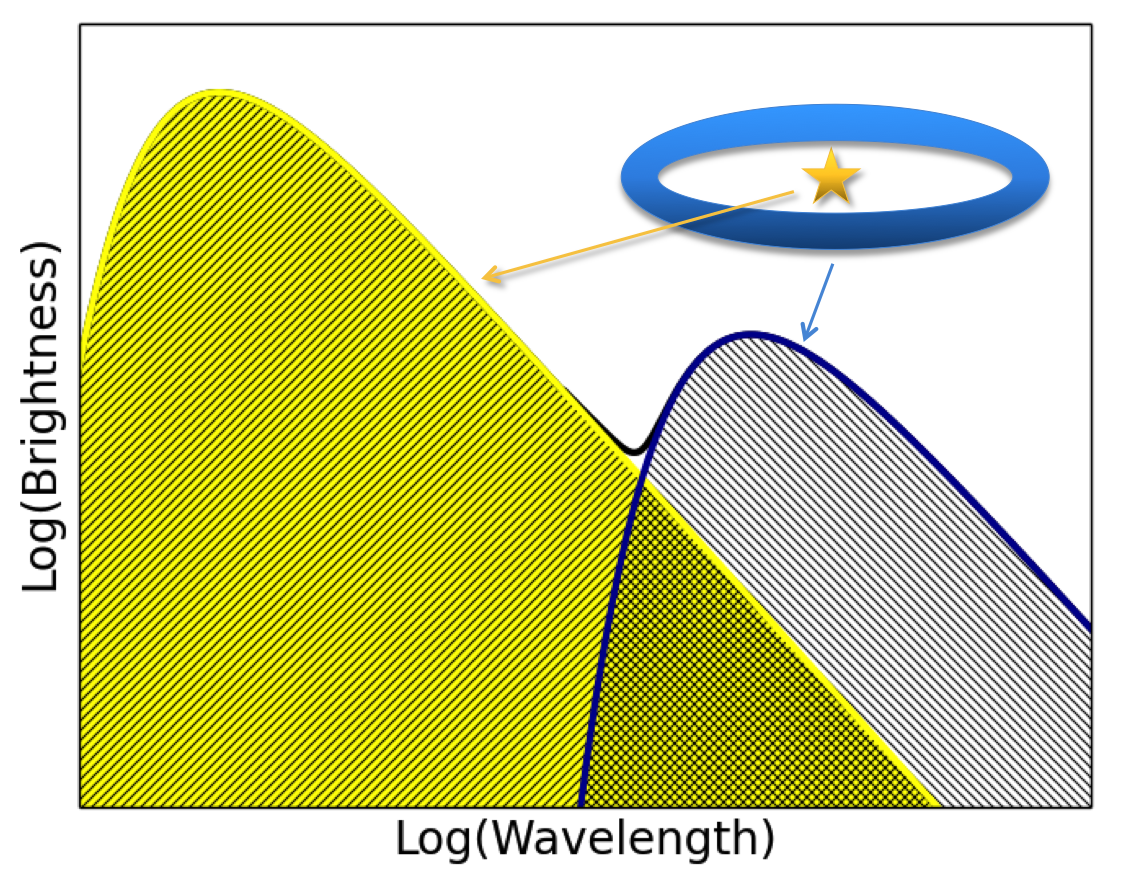
\includegraphics[width=0.7\textwidth]{49CET_SED_Cartoon_StarInsideDisk.png}
\caption{A representation of the SED of a star with a debris disk on a log-log plot. The star dominates at short wavelengths, whereas the disk emits the bulk of its radiation at longer wavelengths. Idea for cartoon courtesy of \cite{Stee14}.}
\label{fig:49CET_SED_Cartoon}
\end{figure}

These so-called ``debris disks" mark the final stage of disk evolution. They are characterized by optically thin dust emission and often do not exhibit any detectable gas emission. Because the lifetime of dust is generally on the order of tens of thousands of years \citep{Su13}, the grains in debris disks are assumed to be secondary, replenished through collisions of planetesimals. In order to excite rocky bodies to destructive collisional velocities, a stirring mechanism is needed. The gravitational influence of a planet can be responsible, but so-called ``self-stirring" is also possible, in which $\sim$ 1000\,km sized planetesimals coalesce before initiating a collisional cascade that results in small dust grains \citep{Keny04, Keny08, Must09, Moor13}. As a result of these stirring mechanisms, belts similar to the Solar System's asteroid and Kuiper belts are common in debris disks. 



These disks are usually identified by their fractional infrared excesses, $\sfrac{L_{IR}}{L_{bol}}$. \cite{Auma84} first noted this phenomena using the Infrared Astronomical Satellite (\textit{IRAS}), correctly attributing the excess to thermal emission of circumstellar grains heated by ultraviolet and visible light from the central star. As seen in Figure \ref{fig:49CET_SED_Cartoon}, the star dominates emission at short wavelengths, but the dust in the disk is brighter at longer wavelengths. Most searches for gas in debris disks have come up empty handed, supporting our assumption that gas and dust evolve simultaneously, but there are a handful of systems that break the norm. 
%relative contribution of small and large grains?

\section{Gas in Circumstellar Disks}

\subsection{Observing Gas in Disks}
In order to analyze the gas content of circumstellar material, observations look for both absorption and emission lines, with each able to reveal different aspects of the gas disk morphology. Temporally stable absorption lines with no velocity relative to the star give insight into the column density of the edge-on gas disk, whereas variable absorption and emission at a variety of relative velocities imply the presence of falling evaporating bodies \citep[FEBs,][]{Beus94} and help constrain the chemistry of the disk. In addition, resolved observations of the gas at millimeter wavelengths and complex modeling have revealed the size, scope, and properties of the gas disk. 

Hydrogen, despite being the dominant component of circumstellar disks, is difficult to observe. The ro-vibrational and rotational lines in the mid-IR are weak, and the strong electronic transitions emit in the ultraviolet where Earth's atmosphere is opaque \citep{Haba05}, though space-based observations are sensitive to these lines. Carbon monoxide (CO) is the most abundant molecule in circumstellar disks other than hydrogen, and it has strong rotational transitions at sub-millimeter and millimeter wavelengths, making it an ideal probe with which to analyze the gas content. Traces of other volatiles such as HCN, HCO+, CN, C$_{2}$H, NH$_{4}$, and polycyclic aromatic hydrocarbons (PAHs) have been detected in disks and help explore the gas disk chemistry \citep{Berg09}, but very low abundances make these observations taxing on telescope resources \citep{Viss11}.

\subsection{Gas-rich Debris Disks}

Using CO as the tracer, observations have shown that the bulk of primordial gas dissipates within $\sim$ 10\,Myr, with less than a Jupiter mass generally remaining after only a few Myr \citep{Zuck95}. This dispersal timescale lines up well with that for dust dispersal from protoplanetary systems, corroborating the view that gas and dust evolve together. However, the existence of gaseous debris disks, which display the secondary dust content of optically thin debris disks but retain enough molecular gas to be detectable at millimeter wavelengths, hints that other processes can shape the gas disk at later stages of disk evolution.  

Gas has been detected in edge-on debris disks with both far-UV \citep[$\beta$ Pic, $\sigma$ Her,][]{Robe00,Chen03} and optical spectra \citep[HD 32207, HD 172555,][]{Redf07,Kief14}. In $\beta$ Pic, stable absorption lines were detected in both CO and C\upperRomannumeral{1}, and a variable component was discovered in C\upperRomannumeral{1}. $\sigma$ Her shows signs of a radiatively driven wind that is blue-shifting gas liberated from collisions between parent bodies at $\sim$ 20\,AU. The optical photometry used by \citeauthor{Redf07} examined strong sodium lines to discover stable absorption by the gas in HD 32207, whereas \citeauthor{Kief14} inferred the presence of FEBs in HD 172555with variable Ca absorption lines. The proximity of $\beta$ Pic ($\sim$ 10\,pc) relative to these other systems has allowed its gas disk to be easily resolved by sub-millimeter observations \citep{Wiln11,Dent14}. Other than the disk around 20\,Myr old $\beta$ Pic, only a small selection of other gas-rich debris disks have been observed via emission spectroscopy of CO at millimeter wavelengths \citep[5\,Myr old HD 141569, 30\,Myr old HD 21997, 40\,Myr old 49 Ceti,][]{Wein00,Moor13,Kosp13, Zuck95}. Until this work, only HD 21997 has been resolved in both gas and dust emission at millimeter wavelengths, though the gas disk around 49 Ceti has been resolved in CO emission \citep{Hugh08}. These systems, taken together, provide a timeline to examine what processes are shaping the gas and dust as disks evolve, but each displays unique properties, indicating that this picture is not a simple one. 

49 Ceti sets the endpoint for describing the evolution of gas in debris disks, although it was not always known to be the oldest of these systems. For some time, it was thought to be 7.8\,Myr old based on evolutionary tracks that simultaneously considered accretion history \citep{Sies00,Thi01b}, but \cite{Rhee07} noted that 49 Ceti's galactic motions with respect to the Sun were not indicative of youth and suggested an age of 20\,Myr. With the classification of 49 Ceti as part of the Argus Association \citep{Zuck12}, this estimate was revised to its current best estimate of $\sim$ 40\,Myr, making it the oldest known main sequence star to contain a substantial reservoir of molecular gas. 

%The ages of these systems are significantly longer than the lifetimes of the constituent materials, so the fact that we see gas at all hints there might be secondary processes releasing gas in a small selection of systems. 

%\cite{Dent95} searched for 12CO around Vega, epsilon Eridanus, Fomalahut, beta leo, and beta pic with J2-1 and J3-2 on JCMT because J1-0 searches had come up empty handed... didn't find any CO emission. need higher sensitivity observations.  

%49 Ceti, an A star, provides a compelling research target, as it is one of only a handful of systems \citep[$\beta$ Pic, HD 21997, HD 141569, ][]{Dent14,Moor13,Kosp13,Wein00} that display the dust properties of optically thin debris disks but retain enough molecular gas to be detectable at millimeter wavelengths. 20 Myr old $\beta$ Pic, also an A star, displays an edge-on gaseous debris disk, and at only 19pc away, it has been studied extensively. Its disk has a dust mass of $\sim 8\times10^{-2}$ $M_{\rm Earth}$ and CO mass of $\sim 4\times10^{-5}$ $M_{\rm Earth}$ \citep{Dent14}. The micron-sized grains revealed in scattered light are essentially co-located with the millimeter grains seen by radio interferometers, with both grain populations peaking at 60\,AU from the star. This nearly matches the inner radius of the gas disk, which extends from 50 to 160 \,AU, peaking at 85 \,AU. Because the CO dissociation timescale is very short ($\sim$ 100 years) in $\beta$ Pic's strong interstellar radiation field, it is likely that the gas is being continually replenished in a ``birth ring" that is also responsible for producing the levels of dust that we see. 

%HD 21997 is a 30 Myr old A star that also hosts a gaseous debris disk. The dust disk extends from 55 to 150 \,AU and has a mass of $\sim 9\times10^{-2}$ $M_{\rm Earth}$ \citep{Moor13}, whereas an estimated $\sim 6\times10^{-2}$ $M_{\rm Earth} of CO extends from $\sim 25$ \,AU to  $\sim 140$ \,AU \citep{Kosp13}. Although the dust and gas disks overlap between 55 and 140 \,AU, within 55 \,AU there seems to be a dust-poor inner region. The distinct locations of the gas and dust hint that different processes may be shaping their morphologies. In fact, \citeauthor{Kosp13} suggest the gas is primordial, but \citeauthor{Moor13} hint that the dust is secondary. 

%HD 141569, an A star $\sim$ 110pc away that is 5Myr old, displays CO emission in addition to displaying the qualities of a debris disk. Scattered light imaging by \cite{Wein00} reveals that the disk extends out to $\sim$ 360\,AU with a gap in the disk at $\sim$ 250\,AU. Gaps like these are suggestive of continual clearing and secondary dust production processes. \cite{Brit07} find that the gas emission comes from within $\sim$ 40\,AU of the star, but it is unclear if the dust traces the gas, as the scattered light imaging is only able to see micron-sized grains at greater than $\sim$ 70\,AU and millimeter observations have not been performed. 

\section{49 Ceti's Gaseous Debris Disk}
\subsection{49 Ceti's Dust Disk}
49 Ceti was first noted as a disk-hosting candidate by \citet*{Sada86}, who correlated objects in the Yale Bright Star Catalog with those that displayed significant 60\,$\mu m$ excesses with \textit{IRAS}. \cite{Jura93} went one step further, showing that 49 Ceti, along with $\beta$ Pic and HR 4796, had $\sfrac{F_{60\,\mu m}}{F_{V}} < 0.1$, implying $\tau~<~10^{-3}$ and thus an optically-thin dust disk. 

%This study will give us a look into whether the gas and dust are dispersing simultaneously and whether the gas is primordial or second generation (created from the collisions of comets), both of which have implications for the timeframe during which giant gas planets can form. 


%Protoplanetary disks, a natural consequence of stellar formation, are planetary nurseries with their huge

%This transitional period is distinguished by an inside-out clearing of sub-mm dust from the star and dispersal of gas from the system which is first identified by a lack of near-IR emission due to the dearth of hot dust close to the star. Photoevaporation by high-energy photons and gravitational clearing by massive planets are the primary mechanisms that disperse the inner dust and gas \citep{Wyat14}. However, transition disks are rare in the stellar neighborhood, as there are few pre-main sequence stars within $\sim$ 100pc. This makes resolved observations, which are needed to confirm the disk morphology, difficult to come by. 

%Understanding this liminal stage is crucial for understanding planet formation. 


%(Something about protoplanetary, debris disks, optical depth differences? see Wyatt 03?)

The spatial distribution of dust was first investigated with Keck imaging at 17.9$\,\mu m$, which revealed low-level emission extending 1.5$''$ (100\,AU) at a position angle of 40$^{\circ}$ \citep{Guil99}, though these data are unpublished. Simultaneous modeling of the mid-IR image and \textit{IRAS} fluxes hinted at a two part disk structure composed of a warm inner component and cold dense outer component. Keck N-band (10$\,\mu m$) images by \cite{Jaya01} marginally resolved extended structure consistent with \citeauthor{Guil99}, but the first sub-arcsecond resolution images of 49 Ceti's disk came from significantly longer exposures with Keck \citep{Wahh07}. These images, at 12.5 and 17.9$\,\mu m$, showed that the disk extended along a NW-SE axis with an inclination of 60$^{\circ} \pm 15^{\circ}$. An optically thin dust disk model with one characteristic grain size was unable to recreate the spatially resolved data and fluxes from the literature, but a model with small grains (a $\sim$ 0.1\,$\mu m$) between 30\,AU and 60\,AU from the star and an extended disk of larger grains (a $\sim$ 15\,$\mu m$) was a good fit. In this model, the undetected outer disk, which contained the majority of the dust mass, was necessitated by the fit to the fluxes at far-IR wavelengths.

Longer wavelength observations of 49 Ceti with Herschel show IR excesses at 70, 160, 260, 350, and 500$\,\mu m$ and resolved extended structure along the major axis at 70$\,\mu m$ \citep{Robe13}. The deconvolved image, with a HWHM of 3.4 arcsec along the major axis, suggests that the semi-major axis of the disk is $\sim$ 200\,AU and shows no signs suggestive of a central clearing or any large-scale asymmetry. 

Attempts to observed the disk in scattered light with the Near-Infrared Camera and Multi-Object Spectrometer (NICMOS) aboard Hubble did not detect any scattered light emission beyond an angular separation of 1.6 arcsec from the central star \citep{Wein99}. This discrepancy will be explored in Section \ref{MidIR}. %Derived fluxes at millimeter wavelengths have thus far been inconsistent with either a thermal spectrum ($F_{\lambda} \propto \lambda^{-2}}$) or optically thin dusty disk spectrum at long wavelengths ($F_{\lambda} \propto \lambda^{-3}}$). \cite{Song04} report a JCMT/SCUBA 850 $\mu m$ flux of 8.2 $\pm$ 1.9mJy, while \cite{Bock94} measured an IRAM 1200$\mu m$ flux of 12.7 $\pm$ 2.3 mJy. Higher signal-to-noise observations at 850 and 1200$\mu m$ will be presented in this work, ironing out this kink in the long-wavelength regime. 

%(a $\sim$ 1$\mu$m) between 30\,AU and 60\,AU from the star are responsible for the majority of mid-infrared excess, whereas an extended disk of larger grains (a $\sim$ 15$\mu$m) is responsible for the rest of the infrared excess. 

\subsection{49 Ceti's Gas Disk}

The molecular gas content of 49 Ceti's disk has been both detected with single radio dishes and resolved with interferometric observations. \cite{Zuck95} marginally detected the CO J=2-1 line with IRAM, showing 49 Ceti contained a measurable amount of gas. JCMT observations of the CO J=3-2 line set an upper limit on the CO mass of 0.02\,M$_{\oplus}$ \citep{Coul98}, which suggests no more than $\sim$ 200\,M$_{\oplus}$ of H$_{2}$. Hydrogen was observed directly in its lowest rotational transition with SWS/ISO, suggesting a lower limit of 110\,M$_{\oplus}$ \citep{Thi01a}, but \cite{Chen06} and \cite{Carm07} did not confirm this detection with \textit{Spitzer}/IRS and VLT/CRIRES, respectively. Modeling by \cite{Dent05} of updated JCMT CO J=3-2 observations suggested a compact disk inclined at $\sim$ 16$^{\circ}$ or a larger ring ($\sim$ 50\,AU) inclined at 35$^{\circ}$, though the secondary model was unable to recreate the high-velocity wings apparent in the line profile. The first resolved images of the gas disk at arcsecond resolution were obtained using the Sub-Millimeter Array (SMA) by \cite{Hugh08}, showing CO J=2-1 emission around 49 Ceti in Keplerian rotation between 40 and 200\,AU, including a central clearing, potentially consistent with photoevaporation.

\section{49 Ceti's Implications for the Evolution of Circumstellar Material}

49 Ceti's debris disk has never been imaged at millimeter wavelengths, and observations in this regime provide an important tracer of the large grains in disks that probe the distribution and dynamics of parent planetesimals. In addition, previous examinations of the gas disk were performed at low resolution with low signal-to-noise, whereas higher sensitivity observations can reveal subtle details about the gas morphology. In this thesis, we present new observations from the Combined Array for Research in Millimeter-wave Astronomy (CARMA) and the Atacama Large Millimeter Array (ALMA) that resolve the extended dust disk at sub-arcsecond resolution for the first time (the gas analysis will be described elsewhere). The level of detail now available in constraining the location, mass, and dynamics of planet forming material with these observations gives us fresh insight into the mechanics that shape circumstellar disks at this late stage of disk evolution. In consideration with other systems, we are helping to complete the picture of how and why gas and dust disperse, which has important implications for the timescale of giant planet formation. Ultimately, making sense of the processes that shape these disks are essential for understanding how solar systems such as our own formed, and will help us figure out how ordinary or rare our Solar System really is. 

%Unraveling these mysteries requires a careful consideration of all pieces of evidence, and our analysis of 49 Ceti is helping us connect the dots to see the big picture.


%which in turn (has implications for) how 

%These systems, taken together, provide somewhat of a timeline to examine what processes are shaping the gas and dust as disks evolve, but each display unique properties, indicating that this picture is in no way a simple one. 

%gives us insight into whether the dust and gas is primordial or secondary. In addition, analysis in combination with younger gaseous debris disks will give us insight into the timescale for giant planet formation. 

%\ifthenelse{\isodd{\thepage}}{\clearemptydoublepage}{}

\chapter{Observations}
\label{chap:obs}

\chapter{Results}
\label{chap3}

\section{CARMA}
\label{CARMAResults}
Figure \ref{fig:CARMA_image} displays the image of 49 Ceti at 1300\,$\mu m$. While there was not a statistically significant detection of the disk on each night, combining all seven nights resulted a 4$\sigma$ detection at the expected position of the star. The image is weighted according to the Briggs weighting scheme with robust = 0.5, which combines the advantages of both natural and uniform weighting. Natural weighting (robust = 2.0) gives lower weights to data with higher noise, which are generally from the longest baselines. This results in a decrease in spatial resolution but greater sensitivity. Uniform weighting (robust = -2.0) gives equivalent weight to all data points, maximizing the spatial resolution but decreasing sensitivity. With robust = 0.5, we have a good balance between resolution and sensitivity in the image. 

\begin{figure}[ht]
\centering
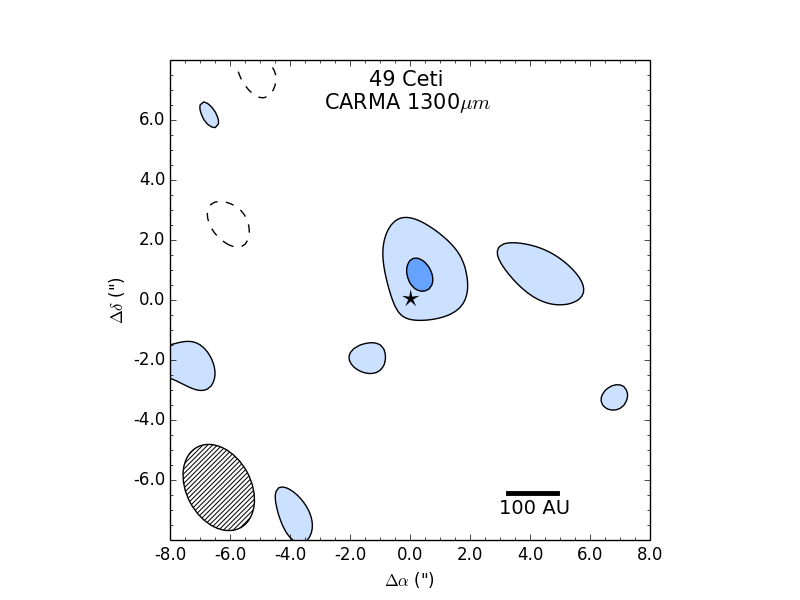
\includegraphics[width = 1\textwidth]{49CET_CARMA_16x16_1300um.png}
%\includegraphics{bonusBelt_200x600_KNAC_TriplePlot_highres.png}
\caption{1300$\mu$m CARMA image of the dust disk of 49 Ceti. The contours are [$-$2, 2, 4] $\times$ 520\,$\mu$Jy/beam (the RMS noise of the image). The beam size, represented by the shaded ellipse in the bottom left corner, corresponds to the resolution of the image, and is 3.04 $\times$ 2.17 arcsec. The position angle of the beam is 28.0$^{\circ}$. The scale bar of 100AU corresponds to 1.64 arcsec on the sky.} 
\label{fig:CARMA_image}
\end{figure}

%The optical depth of the disk can be estimated as the ratio of the infrared luminosity to the bolometric luminosity of the star. In 49 Ceti's case, photometric data from the literature suggest an optical depth of $10^{-3}$ for the dust, which is clearly optically thin. As such, we can

%The ratio of the infrared luminosity excess to the bolometric luminosity suggests 49 Ceti's dust disk is optically thin, and the double-peaked shape that is apparent in the SED (see figure SED) is consistent with a 

The structure of the disk is unresolved by CARMA, but we are still able to glean a reliable flux measurement by fitting a point source to the visibilities with the MIRIAD command \texttt{uvfit}. The derived flux is $2.1 \pm 0.7$\,mJy. If we fit with a Gaussian instead, we find that the major and minor axes are $1.6 \pm 1.8$ arcsec ($100 \pm 110$\,AU) and $0.3 \pm 1.7$ arcsec ($20 \pm 110$\,AU), respectively, indicating that the disk is unresolved along both the minor and major axis. 

\section{ALMA}
Figure \ref{fig:49CET_image} displays the image of 49 Ceti at 850\,$\mu m$. The image is also weighted using the Briggs weighting scheme, with robust = 0.5. In order to derive the integrated flux density, we fit a Gaussian to the visibilities at baselines $\leq$ 50 kilolambda, as these correspond to the largest angular scales in the data (see Figure \ref{fig:deprojected_DP_PL_Vis} for a plot of the deprojected visibilities). These baselines ``see" a disk that is well described by an elliptical Gaussian, and derive a flux of $17 \pm 3$\,mJy. Fitting a ring to all baselines severely underestimates the integrated flux, as any extended flux component would be missed by this model, but it does let us estimate where the peak emission is in the disk. The major axis of the ring is $3.822 \pm 0.003$ arcsec ($233.0 \pm 0.2$\,AU), and the minor axis is $0.626 \pm 0.003$ arcsec ($38.2 \pm 0.2$\,AU), implying that the structure is resolved along both the major and minor axes. The radius of this ring corresponds to the length of the semi-major axis and suggests that the brightest part of the disk is at roughly 117\,AU from the star. In addition, if we assume the disk is circular, we can derive the inclination. Denoting $a$ and $b$ the major and minor axes as seen by the observer and $i$ the inclination,

\begin{equation}
b = a \times sin (90 - i)
\end{equation}

The derived inclination is $80.6^{\circ} \pm 0.4^{\circ}$. The position angle ($PA$) is $-70.9^{\circ} \pm 0.4^{\circ}$. These values are consistent with those derived from subarcsecond Keck images of the inner disk by \cite{Wahh07}, who found $PA = -55^{\circ} \pm 10^{\circ}$ and $i = 60^{\circ} \pm 15^{\circ}$. They are also consistent with the values of $PA = -70^{\circ} \pm 10^{\circ}$ and $i = 90^{\circ} \pm 5^{\circ}$ derived from the outer gas disk observed with the Sub-Millimeter Array by \cite{Hugh08}.

If the 20$\%$ systematic uncertainty in calibrating the flux for radio instruments is taken into account, there is no statistical difference between the ALMA flux at 850$\,\mu m$ of $17 \pm 3$\,mJy and that from JCMT/SCUBA, also at 850$\,\mu m$, of $8.2 \pm 1.9$\,mJy \citep{Song04}. If we assume either a thermal spectrum ($F_{\lambda} \propto \lambda^{-2}$) or optically thin dust disk spectrum at long wavelengths ($F_{\lambda} \propto \lambda^{-3}$), we can compare the CARMA flux of $2.1 \pm 0.7$\,mJy at 1300$\,\mu m$ to the IRAM flux of $12.7 \pm 2.3$\,mJy derived at 1200$\,\mu m$ by \cite{Bock94}. With a thermal spectrum, we would expect the CARMA flux to be $10.8 \pm 2.0$\,mJy, but if the flux falls off as in an optically thin dust disk, it would be $10.0 \pm 1.8$\,mJy. Either way, there is a statistically significant difference between the IRAM flux and that derived from CARMA. As the error in the IRAM measurement is larger than the value we derived with CARMA, the value reported by \citeauthor{Bock94} is clearly spurious. %Because the values derived in this work are consistent with each other, we use these values later in 

\begin{figure}[ht]
\centering
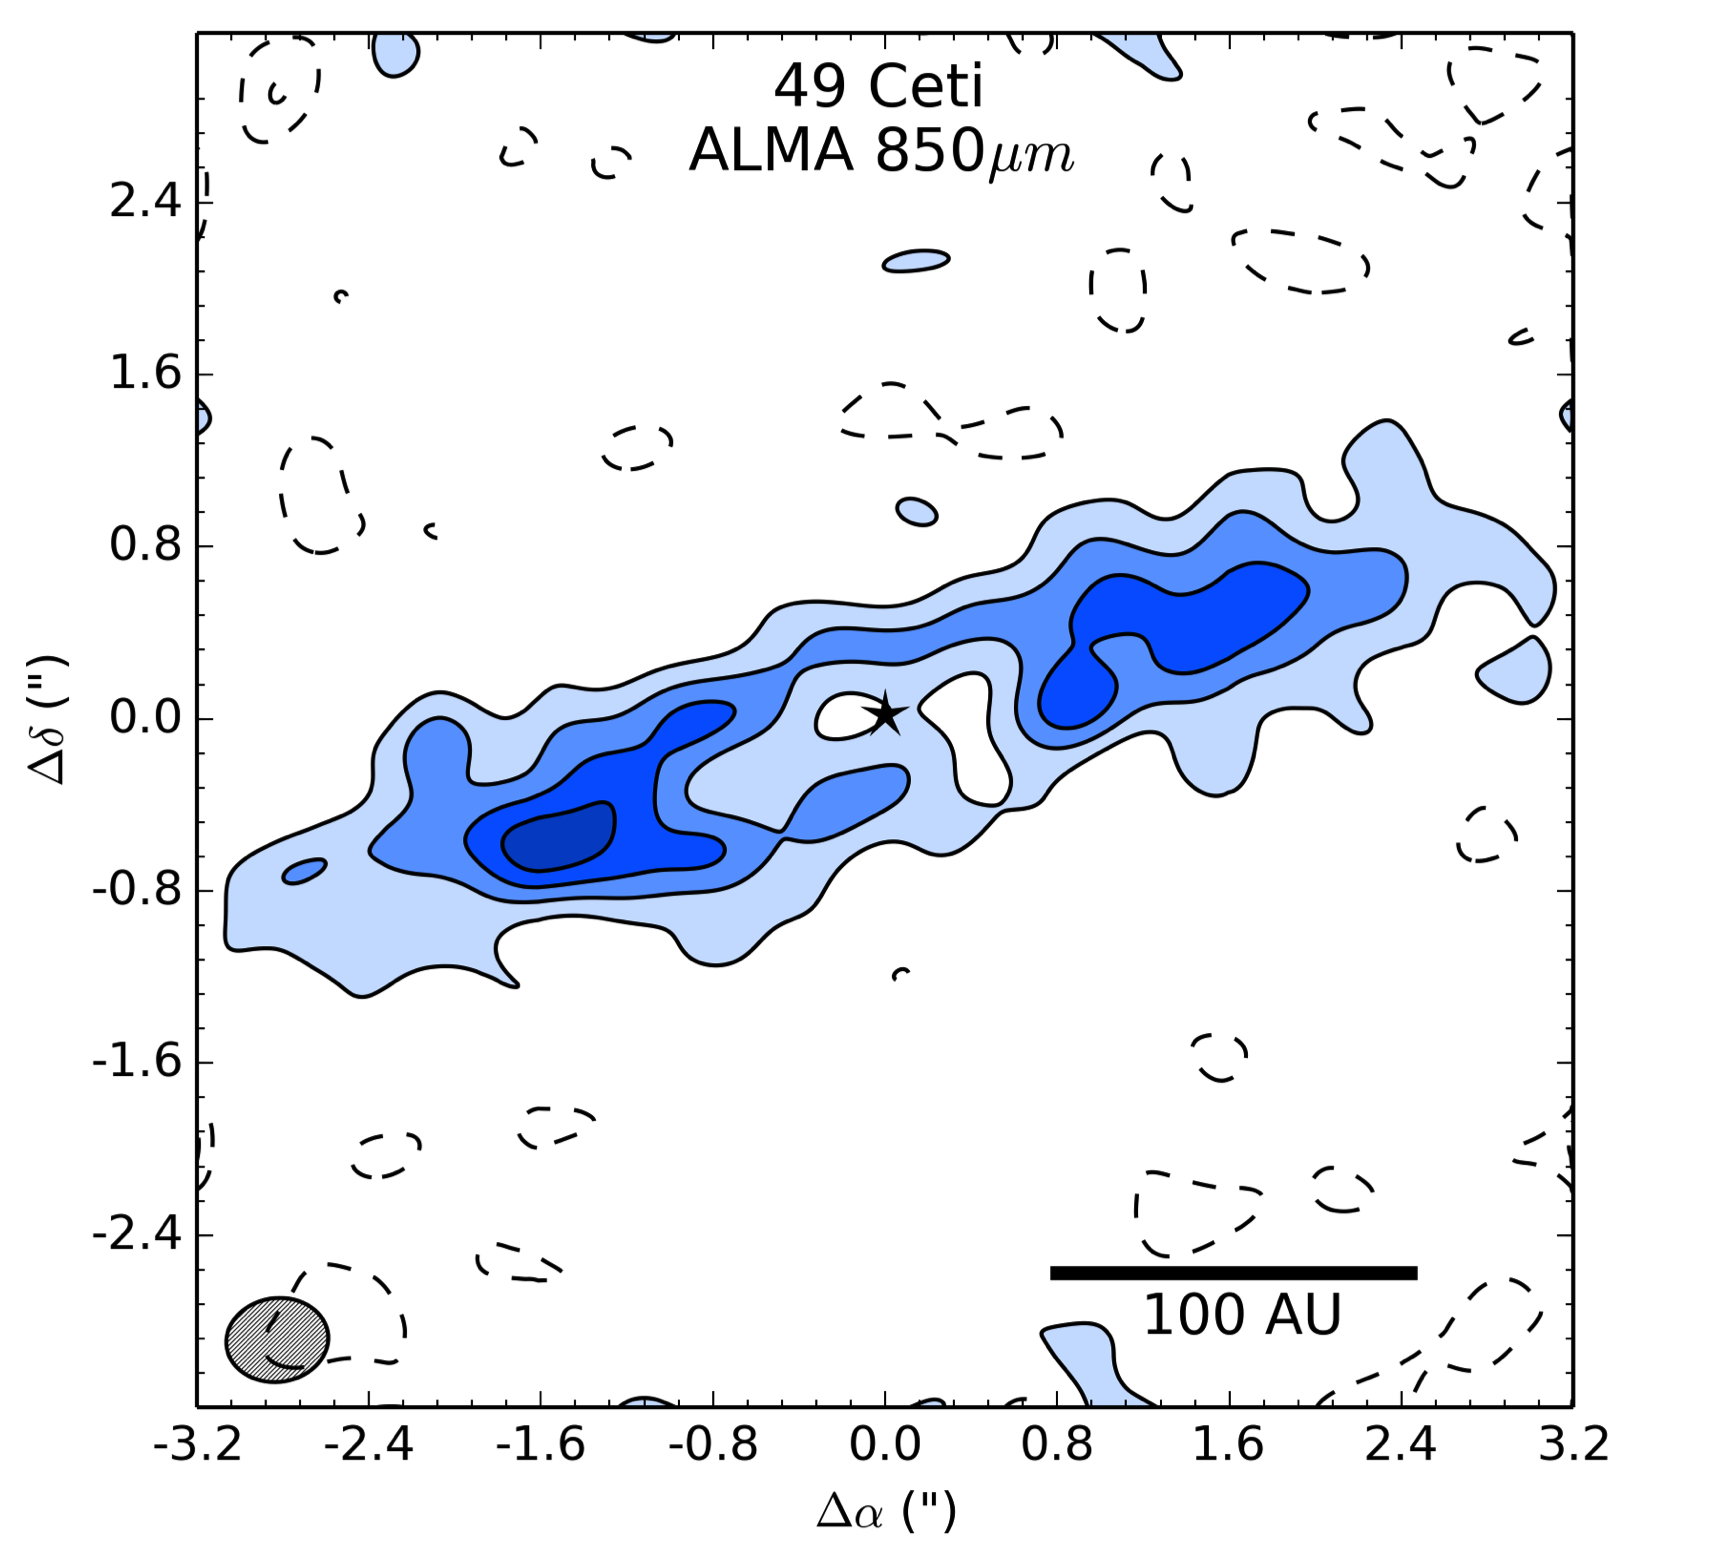
\includegraphics[width = 1\textwidth]{49CET_ALMA_square.png}
%\includegraphics{bonusBelt_200x600_KNAC_TriplePlot_highres.png}
\caption{850 $\mu$m ALMA image of the dust disk of 49 Ceti. The contours are [$-$2, 2, 4, 6, 8] $\times$ 58\,$\mu$Jy/beam (the RMS noise of the image). The beam size, represented by the shaded ellipse in the bottom left corner, is 0.47 $\times$ 0.39 arcsec. The position angle of the beam is -82.7$^{\circ}$. 2$\sigma$ emission extends 195AU from the star, and there seems to be an inner clearing. While the peak emission is slightly higher in the southeast than in the northwest of the disk, this difference is not statistically significant. The separation between the peaks is $\sim$ 3.3$''$ ($\sim$ 200\,AU) in the image and 3.8$''$ ($\sim$ 230\,AU) as derived by fitting a ring to the data with \texttt{uvfit}, suggesting that the density of the dust disk peaks between a radius of 100 and 115\,AU.} 
\label{fig:49CET_image}
\end{figure}




%\ifthenelse{\isodd{\thepage}}{\clearemptydoublepage}{}
%\titlespacing*{\chapter}{0pt}{\baselineskip}{*3}
\chapter{Analysis}
\label{chap4}

We simultaneously model the resolved 850$\,\mu m$ visibilities from ALMA with the unresolved Spectral Energy Distribution (SED) in order to constrain basic geometric properties of the disk and determine the characteristics of the constituent dust grains. The SED, which describes the flux of the system as a function of wavelength, is dominated by emission from the stellar photosphere at $\lambda$ $\lesssim 5\,\mu m$ (for a debris disk), but the dust in the disk contributes the majority of the flux at $\lambda$ $> 5\,\mu m$. The temperature of the grains can be estimated from the wavelength at which the flux peaks, but because grain size and grain location are degenerate from a modeling point of view, characterizing the grain size distribution is impossible without spatially resolved information. Our ALMA data, able to resolve the dust morphology, provide the means with which to break this degeneracy. 

The main factor that determines the appearance of a model disk image is $\Sigma$(r), the surface density as a function of radius. The simplest description of the surface density is with a single power law such that $\Sigma$(r) $\propto r^{-p}$ with abrupt cutoffs at the inner radius ($R_{In}$) and outer radius ($R_{Out}$). This model is presented in Section \ref{SinglePowerSED_Model}. However, 49 Ceti seems to show a ring-like structure at r $\sim$ 100\,AU, suggesting a more complex model of the surface density could provide a better fit. A simple power law with a narrow density enhancement to mimic this ``ring" is discussed in Section \ref{USDE}, and a double power law, with surface density increasing to the radius of this ``ring" before decreasing, is presented in Section \ref{DP}. 

We use the $\chi^{2}$ parameter to determine the goodness of fit for each model and an affine-invariant Markov Chain Monte Carlo (MCMC) fitting process (\cite{Fore13}, \cite{Good10}, described in Section \ref{MCMC}), to obtain a robust, statistical characterization of the model parameters. The complex interferometric points that ALMA measures, called visibilities, are the result of short ($\sim$ 30\,s) integrations. Each independent baseline, of which there are $N(N-1)/2$ of in an array with N antennas (378 from our 28 element array), produces multiple data points for each integration. Multiple spectral windows, each with adjustable channel resolutions, can be find tuned depending on the requirements of the observation. As discussed in Section \ref{ALMA Observations}, three spectral windows, two with 128 channels and one with 3840 channels, were averaged into single data points to make modeling simpler and more efficient. Taking into account the two orthogonal polarizations detected by the ALMA antennas and after removing flagged visibilities (bad data points) we were left with 131400 visibilities. For these data, the $\chi^{2}$ is calculated as:

\begin{equation}
\chi^{2}_{Vis} =  \sum_{i=1}^{131400} w_{i} \bigg[\bigg(d_{i,real} - m_{i,real}\bigg)^{2} + \bigg(d_{i,imag} - m_{i,imag}\bigg)^{2}\bigg] 
\end{equation} 

where $w_{i}$ is the weight from the data associated with visibility $i$, $m_{i,real}$ and $m_{i,imag}$ are the real and imaginary components of the model visibility $i$, and $d_{i,real}$ and $d_{i,imag}$ are the real and imaginary components of the data visibility $i$. The weight $w_{i}$ given to each visibility is related to the antenna temperature of each antenna in a given baseline, the integration time, and the bandwidth of observation. However, the National Radio Astronomy Observatory (NRAO), which oversees ALMA, was having issues with its proprietary software package CASA (Common Astronomy Software Applications) at the time we were reducing the data, resulting in the weights being scrambled when the data were exported. As a result, we had to recalculate the weights directly from the scatter between channels for visibilities in each un-averaged spectral window. This is possible because the standard deviation from the mean over all channels for each visibility, $\sigma_{i}$, determines $w_{i}$, as $w_{i} = \sfrac{1}{\sigma_{i}^{2}}$. In other words, high quality data points, with only a small amount of scatter between the channels, will have a greater effect in describing the goodness of fit of a given model. 

For the SED, we only fit to data points at wavelengths greater than 5$\,\mu m$, as this is the regime in which the disk contributes a significant flux to the total. A total of 19 points were fit to in the SED until additional photometry from \cite{Robe13} were discovered, at which point 30 points were fit to. Then, the disk $\chi^{2}$ is calculated as:

\begin{equation}
\chi^{2}_{SED} =  \sum_{i=1}^{19~\text{or}~30} \big(\frac{F_{\lambda_{i},model} - F_{\lambda_{i},data}}{\sigma_{\lambda_{i}}}\big)^{2}
\end{equation} 

where $F_{\lambda_{i},model}$ is the model flux, $F_{\lambda{i},data}$ is the data flux, and $\sigma_{i}$ is the error for a measurement at $\lambda_{i}$. The uncertainties associated with the SED data points are small compared with those associated with each visibility, but the large number of visibilities relative to the number of SED fluxes means that each contributes roughly equally to the final result of a simultaneous fit for a suitable model. 

%each ends up contributing almost equally to the final result in a simultaneous fit. 


%With these data constraining the location of the emitting grains and the SED determining the temperature of the grains in a simultaneous model, 
%, but at longer wavelengths, emission from grains in the disk dominate, as the dust grains absorb energetic stellar radiation, heat up, and re-emits a portion of the energy at a wavelength that is dependent on 

\section{Markov Chain Monte Carlo Simulations}
\label{MCMC}

In order to analyze how successful our models are and explore the uncertainties associated with each parameter, we utilize the affine-invariant Markov chain Monte Carlo (MCMC) fitting technique as described by \cite{Good10} and implemented in Python as \texttt{emcee} by \cite{Fore13}. Using a MCMC method allows us to probabilistically sample the full parameter space described by our models, obtain a best-fit result, and get statistically robust error bars by characterizing the full posterior distribution function for each parameter. 

This process works by unleashing a series of model ``walkers," with values for parameters in each model sampled as Gaussians around a user-specified center position (a best guess, generally) and user-specified width. $\chi^{2}$ values are calculated for each model, and the walkers move around parameter space, with the probability of the move being accepted related to the total $\chi^{2}$ of that model. If the $\chi^{2}$ is lower for the next step, the move is accepted. If the $\chi^{2}$ is higher, the probability of that move being made is $e^{-(\sfrac{\Delta \chi^{2}}{2})}$, with $\Delta \chi^{2}$ = $\chi^{2}_{original}$ - $\chi^{2}_{proposed~model}$. Defined as such, models move toward a best-fit from their original locations in parameter space while filling out a full posterior distribution function for each parameter. The position of each walker in parameter space along with its corresponding $\chi^{2}$ for all steps is called a ``chain," and is saved for further use. \texttt{emcee} is affine-invariant, meaning moves are only proposed along lines between the walkers. This makes it more efficient at sampling degeneracies between parameters. 

\begin{figure}
\centering
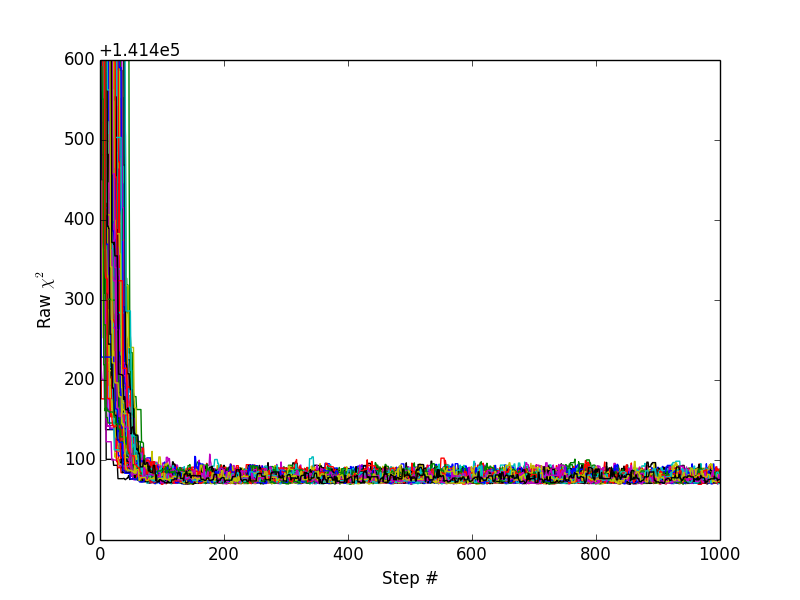
\includegraphics[width = 1\textwidth]{49CET_BurnIn_140x1000_Simplest.png}
\caption{The burn-in and subsequent leveling off of the chi-squared after $\sim$ 100 steps is seen in this plot. Raw $\chi^{2}$ are saved for each step in the chain, and are plotted for each walker (different colors). This burn-in diagram corresponds to the model presented in Section \ref{SinglePowerSED_Model}, which unleashed 140 walkers for 1000 steps.}
\label{fig:49CET_BurnIn}
\end{figure}

\begin{figure}
\centering
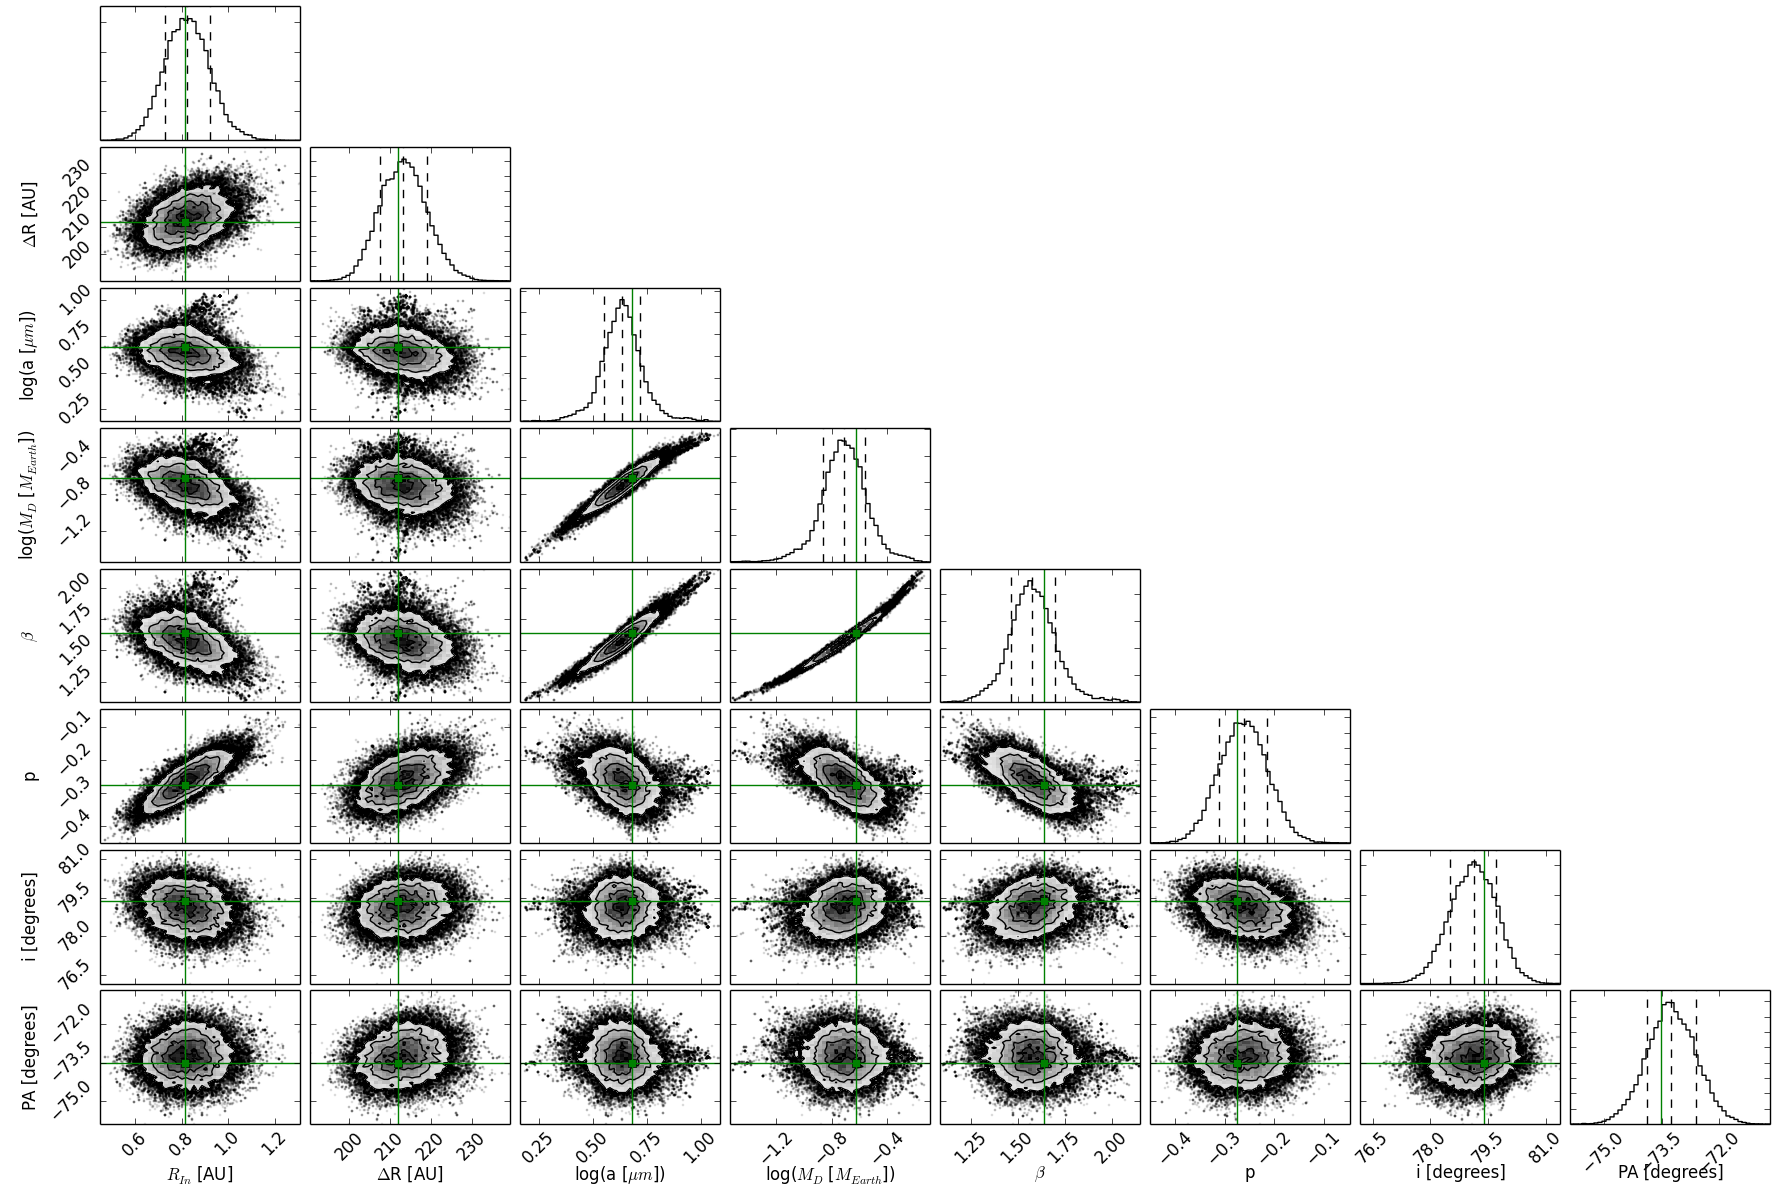
\includegraphics[width = 1\textwidth]{49CET_140x1000_Triangle_150StepBurnIn.png}
\caption{Both one and two dimensional posterior probability distributions for parameters of the single power law model (Section \ref{SinglePowerSED_Model}) as derived from the MCMC chain. The histograms, along the diagonal, display the marginalized distributions for each parameter independently. The dashed lines in the histogram display -1$\sigma$, the median value, and +1$\sigma$ of the distribution, while the green line displays the value of that parameter associated with the overall minimum $\chi^{2}$. The distributions are mostly symmetric. The other plots display the two dimensional marginalized distributions for each pair of parameters and demonstrate the covariances between each pair.}
\label{fig:49CET_Triangle}
\end{figure}

The first $\sim$ 100 steps of an MCMC run compromise the ``burn-in" phase, during which the raw $\chi^{2}$ quickly falls as the walkers move toward the best fit (see Fig \ref{fig:49CET_BurnIn}). This phase tends to be longer if the initial value for one or more of the parameters is far from the correct best-fit value. Before using MCMC, a ``chi-by-eye" fit was performed, with parameters guessed and adjusted until a reasonable fit to the data is found. Then, initial MCMC runs were seeded with wide Gaussians such that the best-fit is somewhere nearby and the MCMC process doesn't have a hard time finding it. Once a best-fit is known, narrower Gaussians are utilized to lessen the burn-in phase.

The median reported value in each table is the most likely value in the MCMC chain once the burn-in phase has been removed; the best-fit value for each parameter corresponds to the global minimum of the total $\chi^{2}$. As the models trace out posterior distribution functions, values $\pm$ 1$\sigma$ from the median value are also reported. We find that the best-fit values are generally within $\pm$ 1$\sigma$ of the median. Figure \ref{fig:49CET_Triangle} shows one and two dimensional posterior distributions from the model presented in Section \ref{SinglePowerSED_Model}.

For all models, disk mass parameters ($M_{Disk}$, $M_{Inner Disk}$, $M_{Outer Disk}$, $M_{Ring}$) and the grain size $a$ are sampled logarithmically, while the rest of the parameters are sampled in a linear fashion.  Visibility-only fits were performed for each model of the surface density such that $\chi^{2}$ = $\chi^{2}_{Vis}$ in order to determine what the spatially resolved data tell us, uninfluenced by the SED. Then, simultaneous fits were performed, with $\chi^{2}$ = $\chi^{2}_{Vis}$ + $\chi^{2}_{SED}$ such that all model parameters could be constrained.

%In Section \ref{SinglePowerSED_Model} we attempted to recreate the data with a standard power law model of the surface density distribution of a geometrically and optically thin dust disk, and while this provided a good fit to the SED, it failed to recreate the visibilities. From the significant positive residuals apparent to the SW side of the disk and negative residuals visible near the center, it was clear that a more complex model describing the surface density was necessary. In Section \ref{MoreComplexModels}, we modeled the surface density both with a double power law, increasing in density to a variable radius before dropping off, and with an unresolved surface density enhancement at a variable radius. Both models were able to recreate the SED, but the SED dominated the fit, skewing the fits to the visibilities. In order to create the significant mass of hot dust necessary to recreate the mid-IR excess, the best-fit results had inner radii within 1AU of the star, resulting in models that were too bright at the center. The unresolved surface density enhancement (USDE???) model was able to account for the ring-like structure, but the double power law model was not, presumably altered by the fit to the SED. 

%To eliminate the contribution of the SED, $\chi^{2}$ values were computed only using the visibilities for both the double-power law and the surface density enhancement. As presented in Section \ref{VisOnly}, we found that both models were able to recreate the density enhancement without becoming too bright at the center. However, as expected, these models didn't contribute enough flux at mid-IR wavelengths. Building upon the results of \cite{Wahh07}, we described an inner disk with a grain size of 0.1$\,\mu m$ and let the characteristic grain size of the outer belt vary. Because small grains radiate at higher temperatures at a given distance from the star than their larger brethren, they were able to boost the mid-IR flux without contributing significantly to the flux at millimeter wavelengths. Both the double power law and unresolved surface density enhancement models with different characteristic grain sizes, presented in Section \ref{ThreePart}, were able to fully recreate our data. 

%Best fit parameters were determined using an affine-invariant Markov Chain Monte Carlo (MCMC) fitting algorithm (\ref{Fore13}, Goodman \& Weare 2010 <<no bibtex for this??, described in Section \ref{MCMC}), a process that provides a robust, statistical characterization of the model parameters. 

%A closer look at the mid-IR spectrum of 49 Ceti gathered from IRS is presented in Section \ref{MidIR}. 

%%%%%%%

\section{Single Power Law Model}
\label{SinglePowerSED_Model}

In order to model a simple geometrically and optically-thin disk model, we follow the approach of \cite{Rica13}, and have the surface density profile $\Sigma(r)$ described by a single power law $p$, with abrupt cutoffs at the inner radius, $R_{In}$, and the outer radius, $R_{Out}$. The surface density is normalized to 100\,AU ($\Sigma_{100\text{AU}}$) and parameterized as:

\begin{equation}\label{eq:sigmaR}
\Sigma(r) = \Sigma_{100\text{AU}}\Big(\frac{r}{100\text{AU}}\Big)^{-p}
\end{equation}

We are able to solve for $\Sigma_{100\text{AU}}$, as we know the integral of the surface density over all infinitesimal rings from $R_{In}$ to $R_{Out}$ must be equal to the total mass of emitting grains in the disk, $M_{Disk}$. 

\begin{equation}\label{eq:mdisk}
M_{Disk} = \int_{R_{In}}^{R_{Out}} \Sigma(r) 2 \pi r \,dr = \int_{R_{In}}^{R_{Out}} \Sigma_{100\text{AU}}\Big(\frac{r}{100\text{AU}}\Big)^{-p} 2 \pi r \,dr
\end{equation}

Integrating and solving for $\Sigma_{100\text{AU}}$, we find:

\begin{equation}\label{eq:sigma100}
\Sigma_{100\text{AU}} = \cfrac{M_{Disk} (2 - p)}{2\pi (100\text{AU})^{p} [(R_{Out})^{2-p}-(R_{In})^{2-p}]}
\end{equation}

Equation \ref{eq:sigma100} lets us vary $p$, $R_{In}$, $R_{Out}$, and $M_{Disk}$. We model $R_{Out}$ as $R_{In} + \Delta R$ to easily ensure that $R_{Out}$ doesn't go within $R_{In}$. Combining these parameters with Equation \ref{eq:sigmaR}, we are able to calculate what the surface density should be at any radius. 

The parameters that describe the dust grains are the characteristic grain size ($a$) and the long-wavelength power law index of grain emission efficiency ($\beta$). We assume that the number of grains of each size is follows the distribution determined in a theoretical collisional equilibrium, i.e. dN $\propto a^{-3.5}$\,d$a$ \citep{Thib07}. The absorption and emission efficiency of a grain as a function of wavelength, $Q_{\lambda}$, is related to size of the grain. Grains are good absorbers and emitters at wavelengths shorter and comparable to their size, but their efficiency drops off as $\lambda^{-\beta}$ at wavelengths larger than their size. We describe $Q_{\lambda} = 1 - e^{-(\frac{\lambda}{2\pi a})^{-\beta}}$, which has $Q_{\lambda} \approx (\sfrac{\lambda}{2\pi a})^{-\beta}$ in the limit of $\lambda$ $>>$ $2\pi a$ and $Q_{\lambda} \approx 1$ when $\lambda$ $<<$ $2\pi a$, which are exactly the properties we desire. 
%%%%%%%%%%%%%%%%%%%%%%%%%%%%%%%%%%%%%%%%%
%%%%%%%%%%%%%%%%%%%%%%%%%%%%%%%%%%%%%%%%%
%%%%%%%%%%%%%%%%%%%%%%%%%%%%%%%%%%%%%%%%%
%%%%%%%%%%%%%%%%%%%%%%%%%%%%%%%%%%%%%%%%%
%%%%%%%%%%%%%%%%%%%%%%%%%%%%%%%%%%%%%%%%%
%%%%%%%%%%%%%%%%%%%%%%%%%%%%%%%%%%%%%%%%%

This parameterization for $Q_{\lambda}$ also mimics a distribution of grain sizes, whereas MCMC analysis would be impossible if we modeled a full distribution of grain sizes due to significant computational inefficiencies. Large values of $\beta$ signify an emphasis on grain sizes $\sim$ $a$, where as smaller values of $\beta$ give more weight to large grains and their emission at longer wavelengths. By smoothly describing the quantum emission efficiency in this way, we end up with a model that is very computationally efficient and is able to recreate the SED with the minimum number of variable parameters. 


%As mentioned earlier, at long wavelengths, the opacity ($\kappa$) of the grains is described by $\kappa \sim \lambda^{-\beta}$ at wavelengths larger than their size\citep{Natt07}.



%This parameterization for $Q_{\lambda}$ has the added advantage that it mimics a distribution of grain sizes, whereas MCMC analysis would be impossible if we modeled a full distribution of grain sizes due to significant computational inefficiencies. Large values of $\beta$ signify an emphasis on grain sizes $\sim$ $a$, where as smaller values of $\beta$ give more weight to large grains and their emission at longer wavelengths. By smoothly describing the quantum emission efficiency in this way, we end up with a model that is very computationally efficient and is able to recreate the SED with the minimum number of variable parameters. 
%%%%%%%%%%%%%%%%%%%%%%%%%%%%%%%%%%%%%%%%%
%%%%%%%%%%%%%%%%%%%%%%%%%%%%%%%%%%%%%%%%%
%%%%%%%%%%%%%%%%%%%%%%%%%%%%%%%%%%%%%%%%%
%%%%%%%%%%%%%%%%%%%%%%%%%%%%%%%%%%%%%%%%%
%%%%%%%%%%%%%%%%%%%%%%%%%%%%%%%%%%%%%%%%%



%Because grains are very inefficient emitters at $\lambda$ $>>$ $2\pi a$, assigning a single grain size for the dust would be insufficient to recreate the contribution of the dust to the SED. 

%\begin{equation}\label{eq:qFn}
%$Q_{\lambda} = 1 - e^{-(\frac{\lambda}{2\pi a})^{-\beta}}$
%\end{equation}

%The combination of these parameters allows us to approximate a grain size distribution; large values of $\beta$ signify a high ratio of small grains to large grains whereas values of $\beta$ close to zero suggest .....which essentially modifies a Rayleigh-Jeans tail to approximate a distribution of grain sizes.  

The temperature of a grain of a given size at a given distance from the star can then be derived by assuming radiative equilibrium between the the stellar radiation absorbed and the energy emitted by the grain. Not taking the albedo of the grains into account, the energy balance is described by:

\begin{equation}\label{EBalance}
\frac{\pi a^{2} L_{\bigstar}}{4 \pi d^{2}} = 4 \pi a^{2} \sigma T_{g}^{4}
\end{equation}

where $a$ is the grain size, $L_{\bigstar}$ is the luminosity of the central star, $d$ is the distance to the grain from the star, $\sigma$ is the Stephan-Boltzmann constant, and $T_{g}$ is the temperature of the grain. Solving for $T_{g}$, we find:

\begin{equation}\label{tEst}
T_{g} \simeq (\frac{L_{\bigstar}}{16 \pi \sigma})^{\sfrac{1}{4}} d^{\sfrac{-1}{2}}
\end{equation}

From this we can see that the temperature of the grains falls off as approximately $d^{\sfrac{-1}{2}}$. However, grains are not perfect absorbers or emitters, and the albedo changes both as a function of wavelength and grain size. To account for this, we model the composition of the dust as compact astrosilicates as described by \cite{Drai03}, and describe the grains' opacity and albedo according to Mie theory (see \citealt{Bohr83}). Taking the absorption and emission efficiency as a function of grain size and wavelength, $Q(a,\lambda)$ into account, the energy balance is described by:

\begin{equation}
\label{eq:fullEBalance}
\frac{1}{4\pi} \int_0^\infty Q(a,\lambda)F_{\lambda}(r,\lambda)\,\mathrm{d}\lambda = \int_0^\infty Q(a,\lambda)B(T,\lambda)\,\mathrm{d}\lambda
\end{equation}

$F_{\lambda}(r,\lambda)$ describes the flux received by a grain at a radius $r$ from the star and wavelength $\lambda$, and $B(T,\lambda)$ is the grains' Planck function. These expressions are numerically integrated to obtain the temperature of a given grain. The left integral is calculated as a function of $a$ at a radius of 50\,AU, and these values are scaled by r$^{\sfrac{-1}{2}}$ to get the value at different radii. The right integral is calculated as a function of both $a$ and $T$. With this setup, we are able to derive an accurate temperature for a grain of size $a$ at a radius $r$ for grains of any size anywhere in the disk. 

%Then, for a grain of size $a$ at a radius $r$, we are able to derive an accurate temperature, thereby allowing the determination  its contribution to the total flux for grains throughout our model of the disk.

We compare our model to the SED of 49 Ceti at observed photometric points gathered from the literature (displayed in Table \ref{tab:SED}) in order to calculate a $\chi^{2}_{SED}$. The SED displays a double-peaked shape (see Figure \ref{fig:49CET_Simple_SED}) that is consistent with emission from a two-belt configuration, with a warm inner belt boosting mid-IR fluxes and a cool outer belt responsible for the second peak at millimeter wavelengths. We model the SED with two components: (1) a Kurucz-Lejeune model photosphere with surface gravity log(g) = 4.5, effective temperature $T_{Eff}$ = 10000K, and solar metallicity Z = 0.01 \citep{Chen06}, and (2) an extended, spatially-resolved debris disk. Points at a wavelength less than 5$\,\mu m$ were not included in the fit, as the disk contributes a negligible flux relative to the star in this regime. 19 points were included in the SED fit for some models before additional photometry was found, at which point all 30 points presented in Table \ref{tab:SED} were used for fitting (all advanced models used for statistical analysis in Section \ref{stats} use all 30 data points). The ALMA flux is not included in the calculation of the SED $\chi^{2}$, as this flux is implicitly included in the creation of the model image at 850$\,\mu m$ that we compare the visibilities to when calculating the visibility $\chi^{2}$. The IRS spectrum originally consisted of 360 points between 5 and 35$\,\mu m$, but was averaged down to 9 for the sake of computational efficiency. The errors reported in the table for these points are the absolute calibration uncertainty (assumed to be 10$\%$ of the flux measurement) and the statistical uncertainty added in quadrature.

\begin{table*}
\caption{Spatially Unresolved Continuum Fluxes Measured for the 49 Ceti System}
%\resizebox{\textwidth}{!}{
\begin{center}
%\begin{multicols*}{2}
%\setlength\columnsep{12pt}
%\def\arraystretch{1}
%\begin{tabular}{1*{5}{c}r}
\begin{tabular}{ccc}
    \hline\hline   
    Wavelength ($\mu m$) & Flux (Jy) & Source & %\multicolumn{1}{p{2cm}}{\centering Number of \\ Antennas} 
    \hline 
    0.38 & 8.68 & Yerkes Observatory, \cite{Cowl69} \\ 
    0.45 & 20.99 & $''$ \\    
    0.55 & 20.52 & $''$ \\     
    1.22 & 9.55 & Michigan Curtis Telescope, \\     
    1.65 & 6.38 & \citet{Houk88} \\     
    2.18 & 3.98 & $''$ \\     
    3.55 & 1.72 & $''$ \\     
    4.77 & 0.96 & $''$ \\
    5.86 & 0.69 $\pm$ 0.07& IRS Spectrum \\ 
    7.07 & 0.48 $\pm$ 0.05&$''$ \\ 
    8.97 & 0.32 $\pm$ 0.03& $''$ \\ 
    11.40 & 0.21 $\pm$ 0.02& $''$ \\ 
    13.90 & 0.18 $\pm$ 0.02& $''$ \\ 
    17.13 & 0.19 $\pm$ 0.02& $''$ \\ 
    20.90 & 0.21 $\pm$ 0.02& $''$ \\ 
    27.21 & 0.35 $\pm$ 0.03& $''$ \\ 
    34.00 & 0.6 $\pm$ 0.1& $''$ \\ 
    11.56 & 0.21 $\pm$ 0.02 & \textit{WISE}, \cite{Wrig10} \\         
    12.0 & 0.33 $\pm$ 0.07 & \textit{IRAS} Faint Source Catalog \\     
    25.0 & 0.38 $\pm$ 0.08 & $''$ \\    
    60.0 & 2.0 $\pm$ 0.4 & $''$ \\     
    100.0 & 1.91 $\pm$ 0.38 & $''$ \\   
    12.5 & 0.20 $\pm$ 0.03 & Keck, \cite{Wahh07} \\   
    17.9 & 0.19 $\pm$ 0.03 & $''$ \\  
    150.0 & 0.8 $\pm$ 0.5 & ISO \\  
    170.0 & 1.1 $\pm$ 0.5 & $''$ \\  
    63.19 & 2.01 $\pm$ 0.35 & Herschel, \cite{Robe13} \\
    70.00 & 2.142 $\pm$ 0.058 & $''$ \\
    72.84 & 1.95 $\pm$ 0.32 & $''$ \\
    78.74 & 1.90 $\pm$ 0.31 & $''$ \\
    90.16 & 1.88 $\pm$ 0.32 & $''$ \\
    145.54 & 1.16 $\pm$ 0.18 & $''$ \\
    157.68 & 0.98 $\pm$ 0.13 & $''$ \\
    160.00 & 1.004 $\pm$ 0.053 & $''$ \\
    250.0 & 0.372 $\pm$ 0.027 & $''$ \\
    350.0 & 0.180 $\pm$ 0.014 & $''$ \\
    500.0 & 0.086 $\pm$ 0.009 & $''$ \\
%    850.0 & ???? $\pm$ ???? & This work \\
    1300.0 & 0.0021 $\pm$ 0.0007 & CARMA, This work \\
        \hline
\end{tabular}
%    \end{multicols*}
    \end{center}
%\end{adjustbox}
\label{tab:SED}
\caption{The 30 fluxes and their corresponding uncertainties gathered from the literature.}
\end{table*}

In addition to describing and fitting the flux contribution of the grains to the SED, we simultaneously create a high-resolution model image of the disk at 850$\,\mu m$, the wavelength of the spatially-resolved ALMA observations. These images have a resolution on the order of 10$\%$ the spatial scale sampled by our longest baseline, i.e. 3\,AU/pixel. However, for the model described in Section \ref{USDE}, which contained a narrow ring, we used model images with a resolution of 1.5\,AU/pixel. These model images are sampled at the same baseline separations and orientations as the ALMA observations using the MIRIAD command \texttt{uvmodel}, allowing us to compare our model disk to the data. We do this in the visibility domain rather than with the data and model images. These images, which have been created from the visibilities using the the non-linear \texttt{clean} algorithm, do not have well characterized uncertainties, whereas the noise is well understood for each visibility in the visibility domain \citep{Schw78_clean}. In addition, fitting to the visibilities preserves information from the longest baselines (corresponding to the smallest angular scales), whereas the resolution of the image is always coarser than the smallest angular scale.
 
% From this process, the noise that is well understood for each visibility in the visibility domain and is hard to  estimate in the image domain \citep{Schw78_clean}, preventing us from characterizing the uncertainties in the image domain.
 

%a non-linear process that doesn't preserve the 
%noise properties of vis weights....
%understand noise in vis but not in image- clean is nonlinear- 
%visibilities preserve info on smallest scales- long baselines - because clean beam is always larger than smallest angular scale in data (somewhat) over all baselines
%weights associated with ......?????????
%Although there are significantly more visibilities (141300) than SED points that we fit to (30), the visibilities have much lower signal-to-noise, meaning the weight that each $\chi^{2}$ has on the final fit is roughly equal. 

\subsection{Visibility-only Fit}
\label{simple_VisOnly}

In order to ascertain what physical parameters can describe the ALMA data, we perform MCMC analysis using only the visibility $\chi^{2}$. As seen in Figure \ref{fig:49CET_Simple_Vis_ModelResidual}, the model is a good fit, with just a small scatter of 2$\sigma$ residuals left in the residual image. We find that large grains ($\sim$ 850$\,\mu m$), which dominate emission at the wavelength of the ALMA image, are not found within $\sim$ 70\,AU, and that the disk extends out to $\sim$ 300\,AU. Without the simultaneous fit to the SED, $M_{Disk}$, $\beta$, and $a$ are not well constrained.

Even though we didn't take the SED $\chi^{2}$ into account in this model, it is an enlightening exercise to examine what the SED looks like with these model parameters. As seen in Figure \ref{fig:49CET_Simple_Vis_SED}, the model seems to fit the secondary peak from the disk emission (just by chance), but is clearly not bright enough in the mid-infrared. A population of hotter dust grains is necessary to recreate this mid-IR deficit. 

\begin{figure}[t!]
\centering
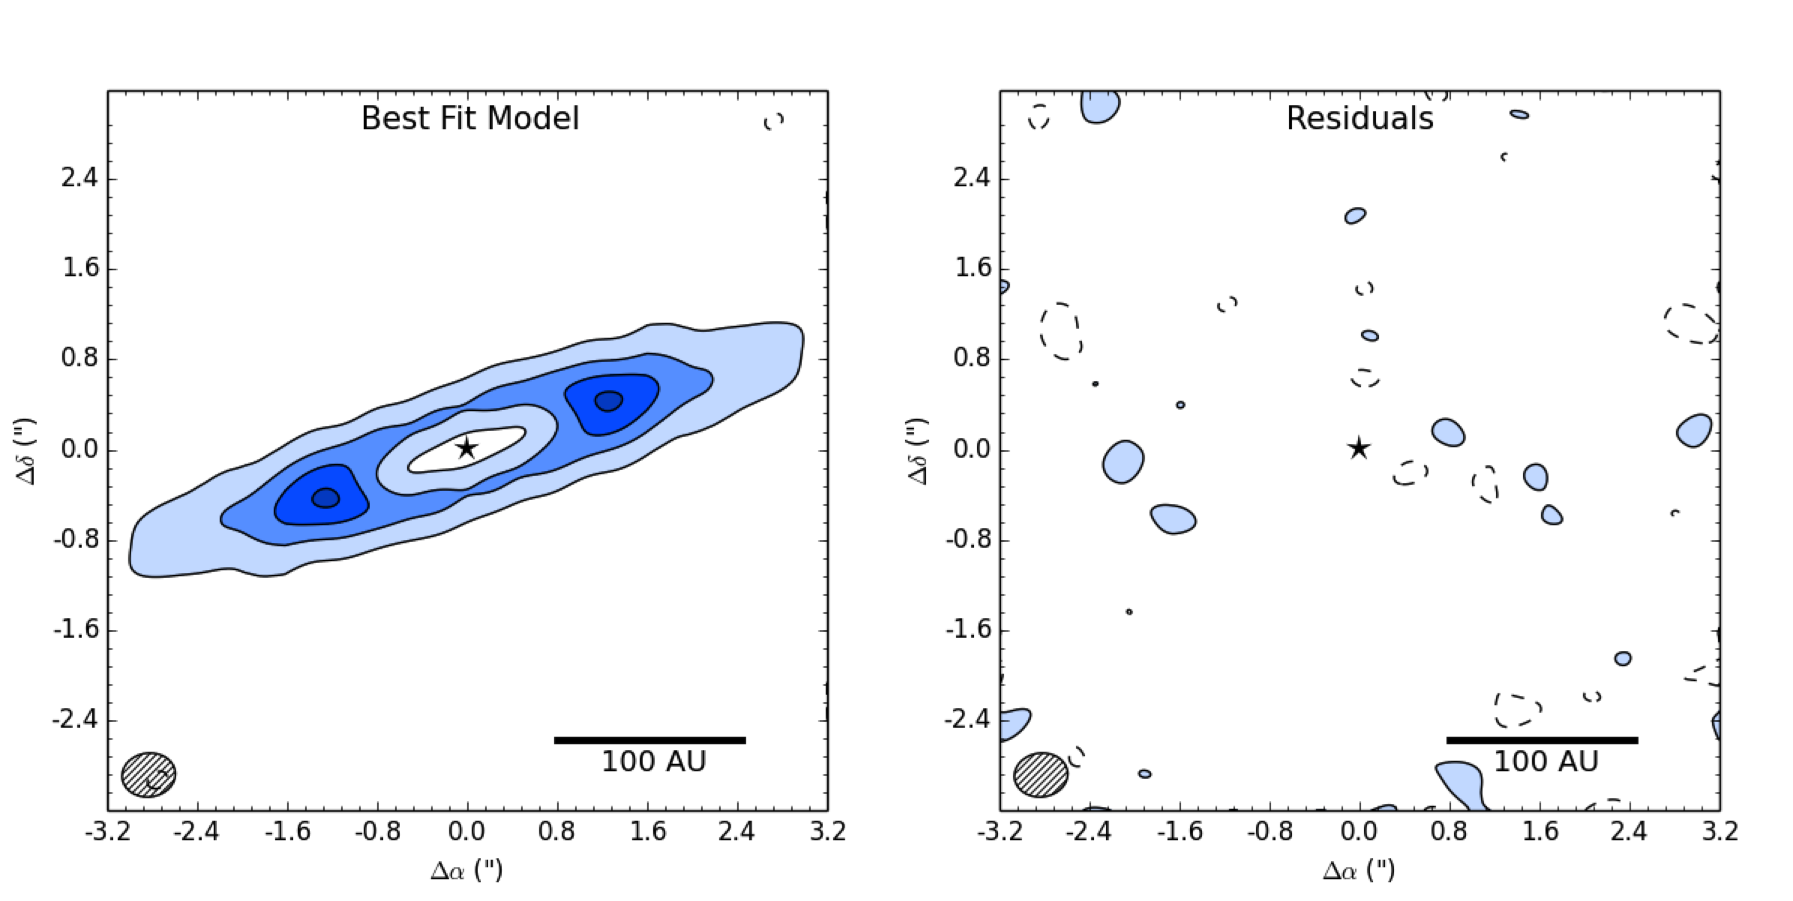
\includegraphics[width = 1\textwidth]{49CET_Simple_Vis_ModelResidual.png}
\caption{The model image (left) and residuals (right) for the single power law model fitting just the visibilities. The residuals are the ALMA visibilities minus model visibilities, subtracted in the visibility domain, then imaged. Contours are [-2, 2, 4, 6, 8] $\times$ 58$\,\mu$Jy (the RMS noise of the data image).}
\label{fig:49CET_Simple_Vis_ModelResidual}
\end{figure}

\begin{figure}
\centering
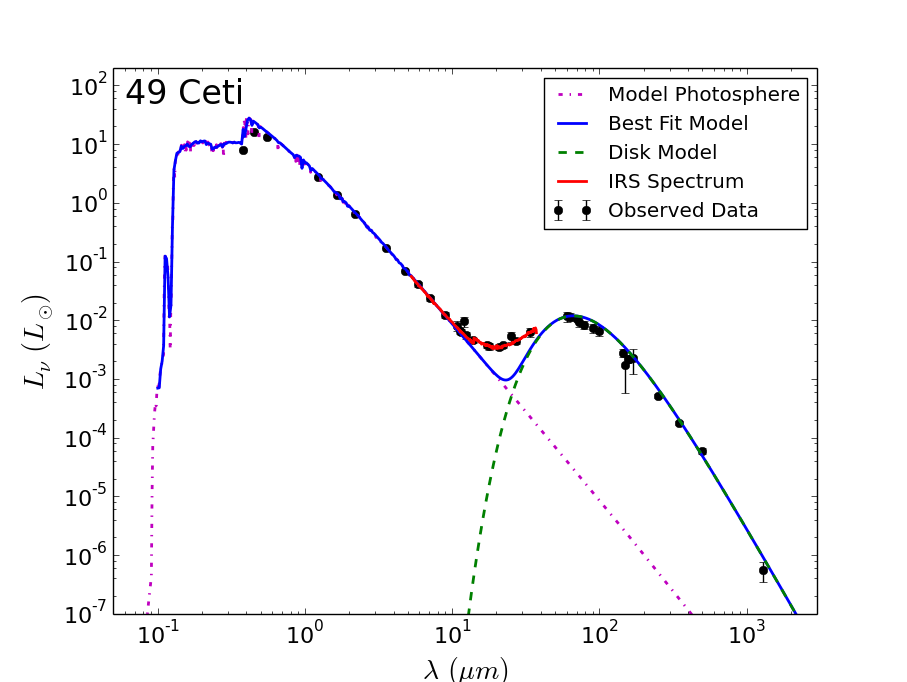
\includegraphics[width = 1\textwidth]{49CET_Simple_Vis_SED_AllData.png}
\caption{The model SED created from parameters derived from the visibility-only single power law fit.}
\label{fig:49CET_Simple_Vis_SED}
\end{figure}

\begin{table}
\begin{center}
    \def\arraystretch{1.37}%
    \begin{tabular}{l*{2}{c}r}
    \hline
    Parameter & Median Value $\pm$ 1$\sigma$ & Best Fit Value \\ \hline
     $R_{In}$  [AU] & 70$^{+3}_{-3}$ & 69\\  
     $\Delta R$ [AU] & 245$^{+9}_{-9}$ & 243\\ 
     log($M_{Disk}$ [$M_{\oplus}$]) & -0.8$^{+0.8}_{-0.8}$ & -0.7 \\
     log(a [$\mu$m]) & 0.8$^{+0.5}_{-0.5}$ & 0.4\\ 
     $\beta$ & 1.4$^{+0.6}_{-0.6}$ & 1.4\\ 
     $p$ & 1.21$^{+0.13}_{-0.17}$ & 1.24\\ 
     $i$ [$^\circ$] & 79.6$^{+0.4}_{-0.4}$ & 79.5 \\ 
     $PA$ [$^\circ$] & -71.3$^{+0.5}_{-0.5}$ & -71.3\\
    \hline
    \end{tabular}
\end{center}
\caption{The median and best fit values for the single power law model fitting only the visibilities.}
\label{tab:49CET_Simple_Vis_Table}
%for all parameters of the model of 49 Ceti's dust disk. THIS IS SIMPLE BONUS BELT, JUST VIS100x840}
\end{table}


\subsection{Simultaneous SED and Visibility Fit}
\label{Simple_SED_Vis}

\begin{figure}[t!]
\centering
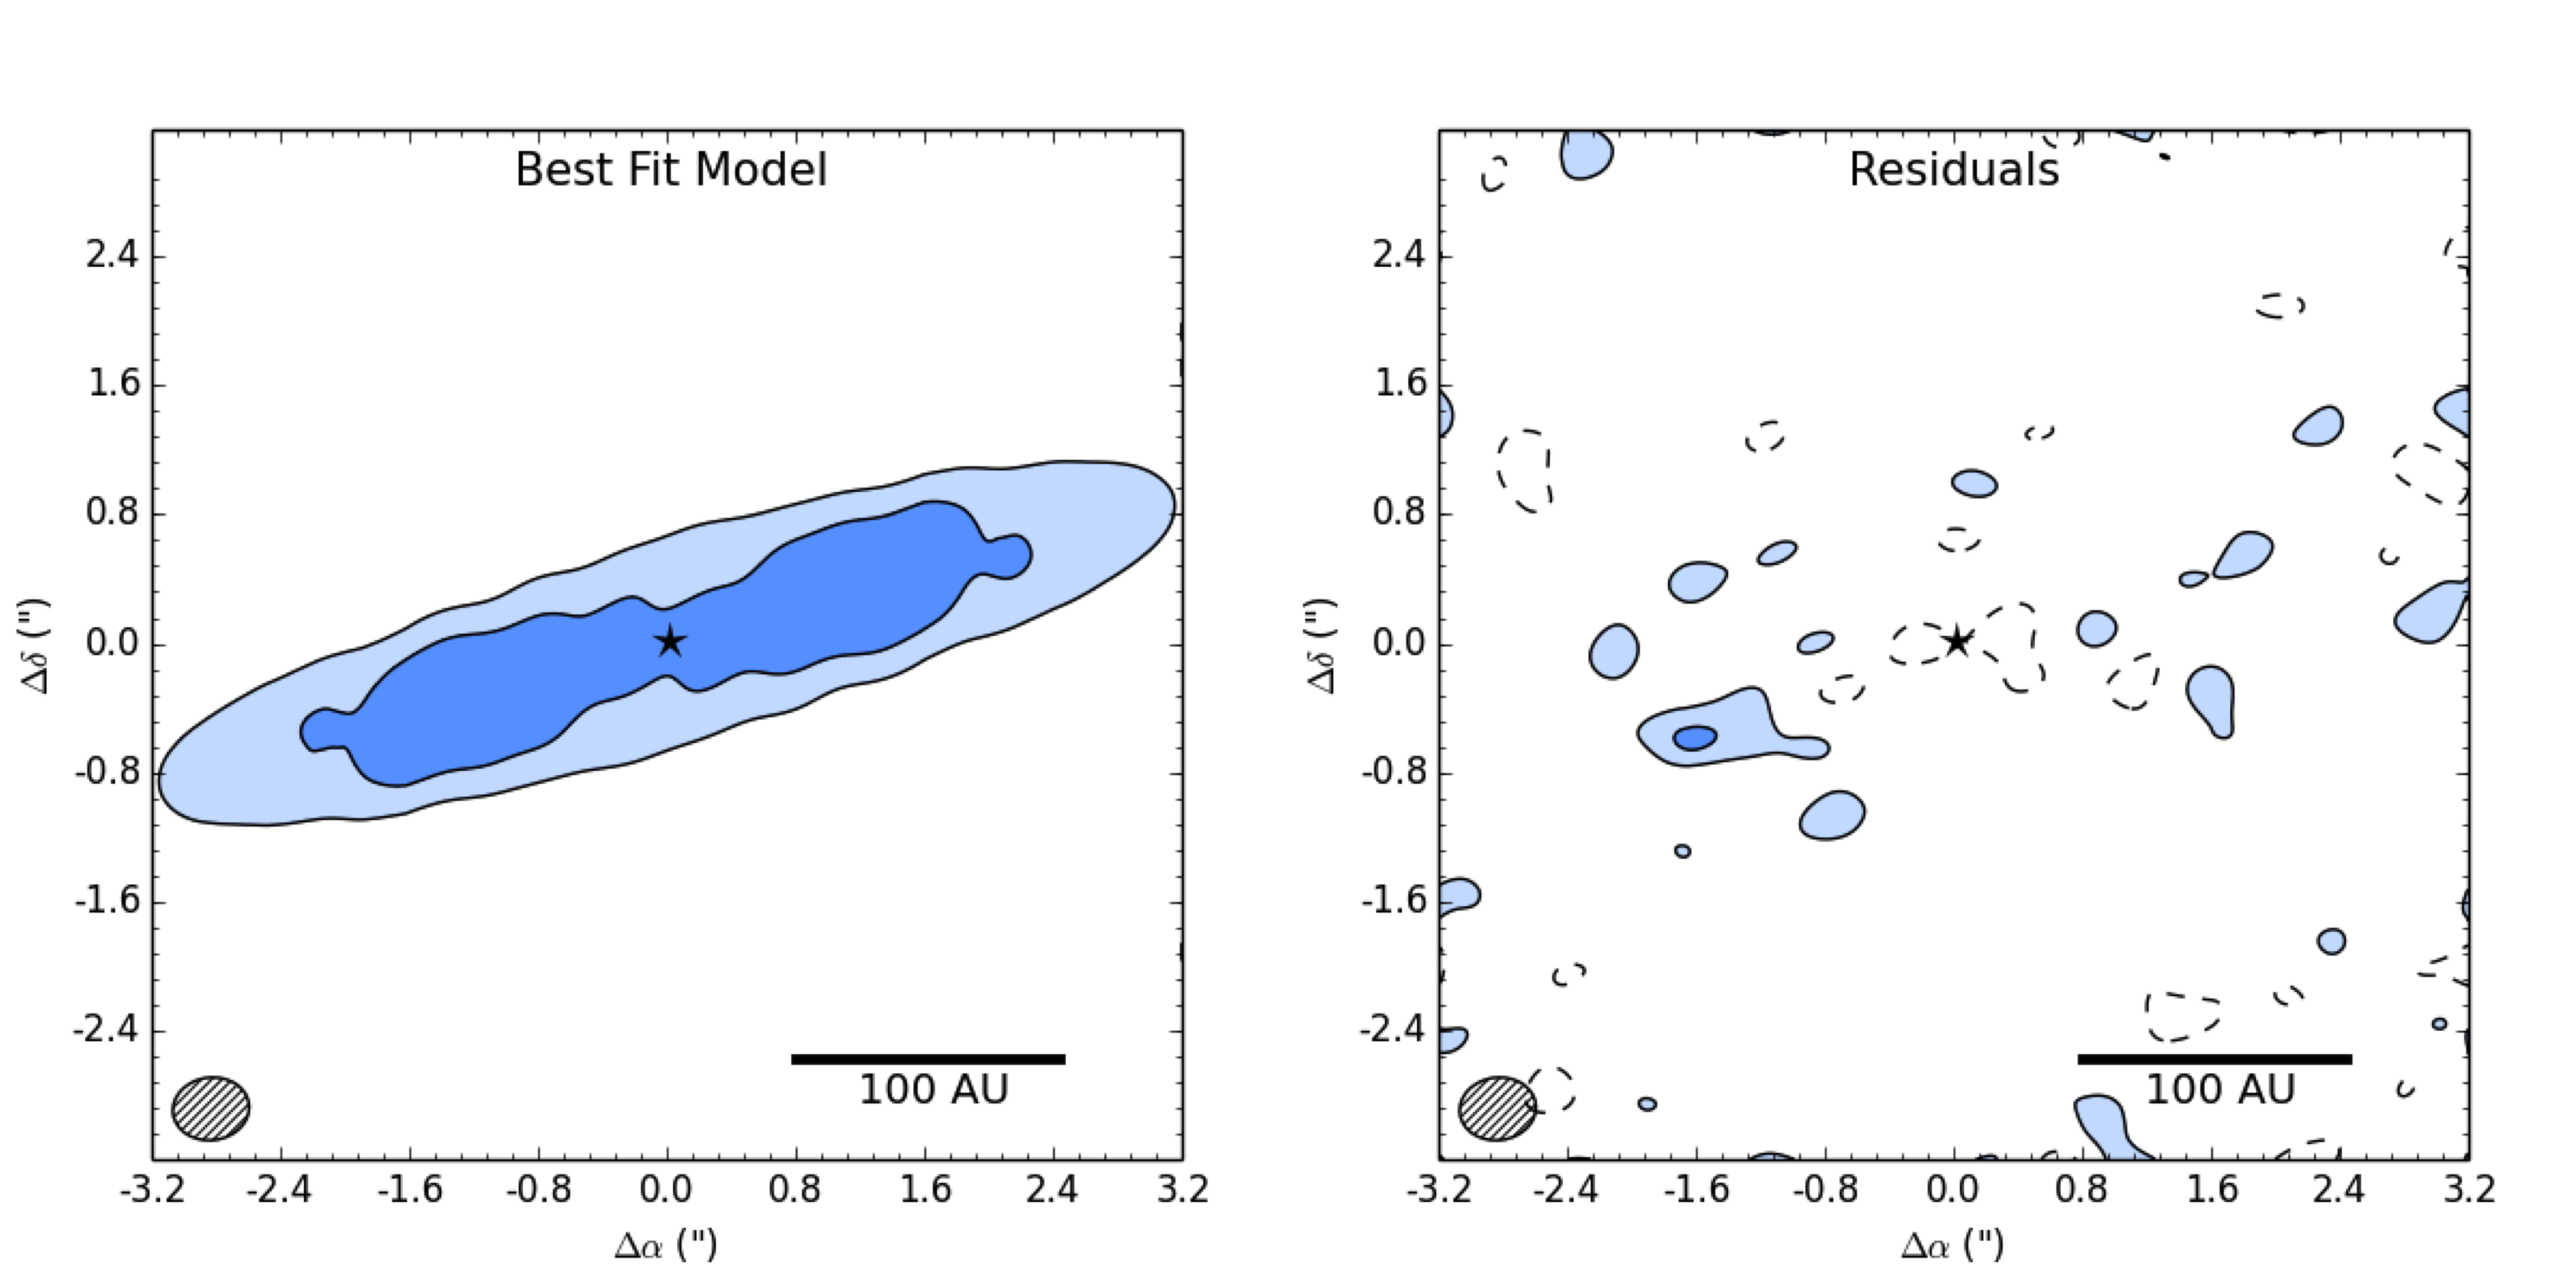
\includegraphics[width = 1\textwidth]{49CET_Simple_ModelResidual.png}
\caption{The model image (left) and residuals (right) for the single power law model fitting to both the SED and visibilities. Contours are [-2, 2, 4] $\times$ 58$\,\mu$Jy (the RMS noise of the data image). The model fails to account for the region of higher density on the southeast side of the disk and leaves residuals in a ring-like pattern around the disk. It is also slightly too bright at the center.}
\label{fig:49CET_Simple_ModelResidual}
\end{figure}

Using the same single power law description of the surface density, we perform a simultaneous fit to both the visibilities and the SED. The best-fit model and residual images are presented in Figure \ref{fig:49CET_Simple_ModelResidual}, the best-fit SED is plotted in Figure \ref{fig:49CET_Simple_SED}, and the parameters are displayed in Table \ref{tab:SimpleModel_Table}. The inner radius in this model is $\sim$ 1\,AU, which has created enough hot grains to recreate the mid-IR fluxes, and the rest of the SED is also a very good fit. However, in doing so, the model has deviated considerably from the value of $p$ that worked well for the visibility-only best-fit model, with $p$ = $-$0.27 now instead of $p$ = 1.24. This difference is clearly due to the influence of the SED and the need for a non-zero inner disk surface density to create hot grains to recreate the mid-IR excess. The shallowly increasing value of $p$ suggests the model is trying to juggle the need of $\Sigma_{Outer Disk} > \Sigma_{Inner Disk}$, and as can be seen in Figure \ref{fig:49CET_Simple_ModelResidual}, this balance is imperfect and results a model disk that is too bright in the center and not bright enough farther out.

%The model leaves 2$\sigma$ residuals in a ring, suggesting the need for a description of the surface density that peaks at a variable radius. It is also too bright near the center of the disk. The median and best-fit values for the single power law  model are presented in Table \ref{tab:SimpleModel_Table}.

\begin{figure}%[!]
\centering
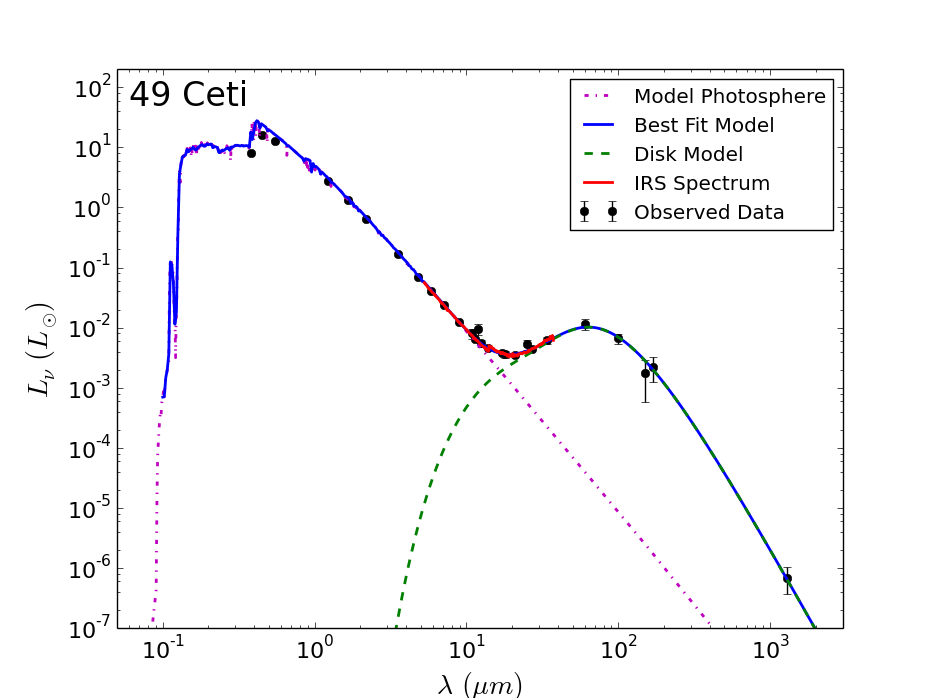
\includegraphics[width = 1\textwidth]{49CET_Simple_SED.png}
\caption{The best fit SED of 49 Ceti for the single power law model simultaneously fitting the SED and visibilities. The best fit model is the sum of the disk model and the model photosphere. Photometric points, excluding those from \cite{Robe13}, are taken from the literature. The full IRS spectrum is presented for display purposes.}
\label{fig:49CET_Simple_SED}
\end{figure}

\begin{table}%[t!]
\begin{center}
    \def\arraystretch{1.10}%
    \begin{tabular}{l*{2}{c}r}
    \hline
     Parameter & Median Value $\pm$ 1$\sigma$ & Best Fit Value \\ \hline
     $R_{In}$  [AU] & 0.82$\pm$0.10 & 0.81\\ 
     $\Delta$R [AU] & 213$\pm$6} & 212 \\ 
     log(a [$\mu$m])  & 0.63$\pm$0.10 & 0.68\\ 
     log($M_{Disk}$ [$M_{\oplus}$])  & -0.71$\pm$0.15 & -0.63\\ 
     $\beta$ & 1.58$\pm$0.12 & 1.64\\ 
     p & -0.26$\pm$0.05 & -0.27\\ 
     i [degrees] & 79.1$\pm$0.6 & 79.4 \\ 
     PA [degrees] & -73.3$\pm$0.6 & -73.5\\
    \hline
    \end{tabular}
\caption{The median values $\pm$ 1$\sigma$ and best-fit values for the single power law model fitting both the SED and the visibilities.}
\label{tab:SimpleModel_Table}
\end{center}
\end{table}

\subsection{Simultaneous SED and Visibility Fit with Two Characteristic Grain Sizes}

\begin{figure}%[t!]
\centering
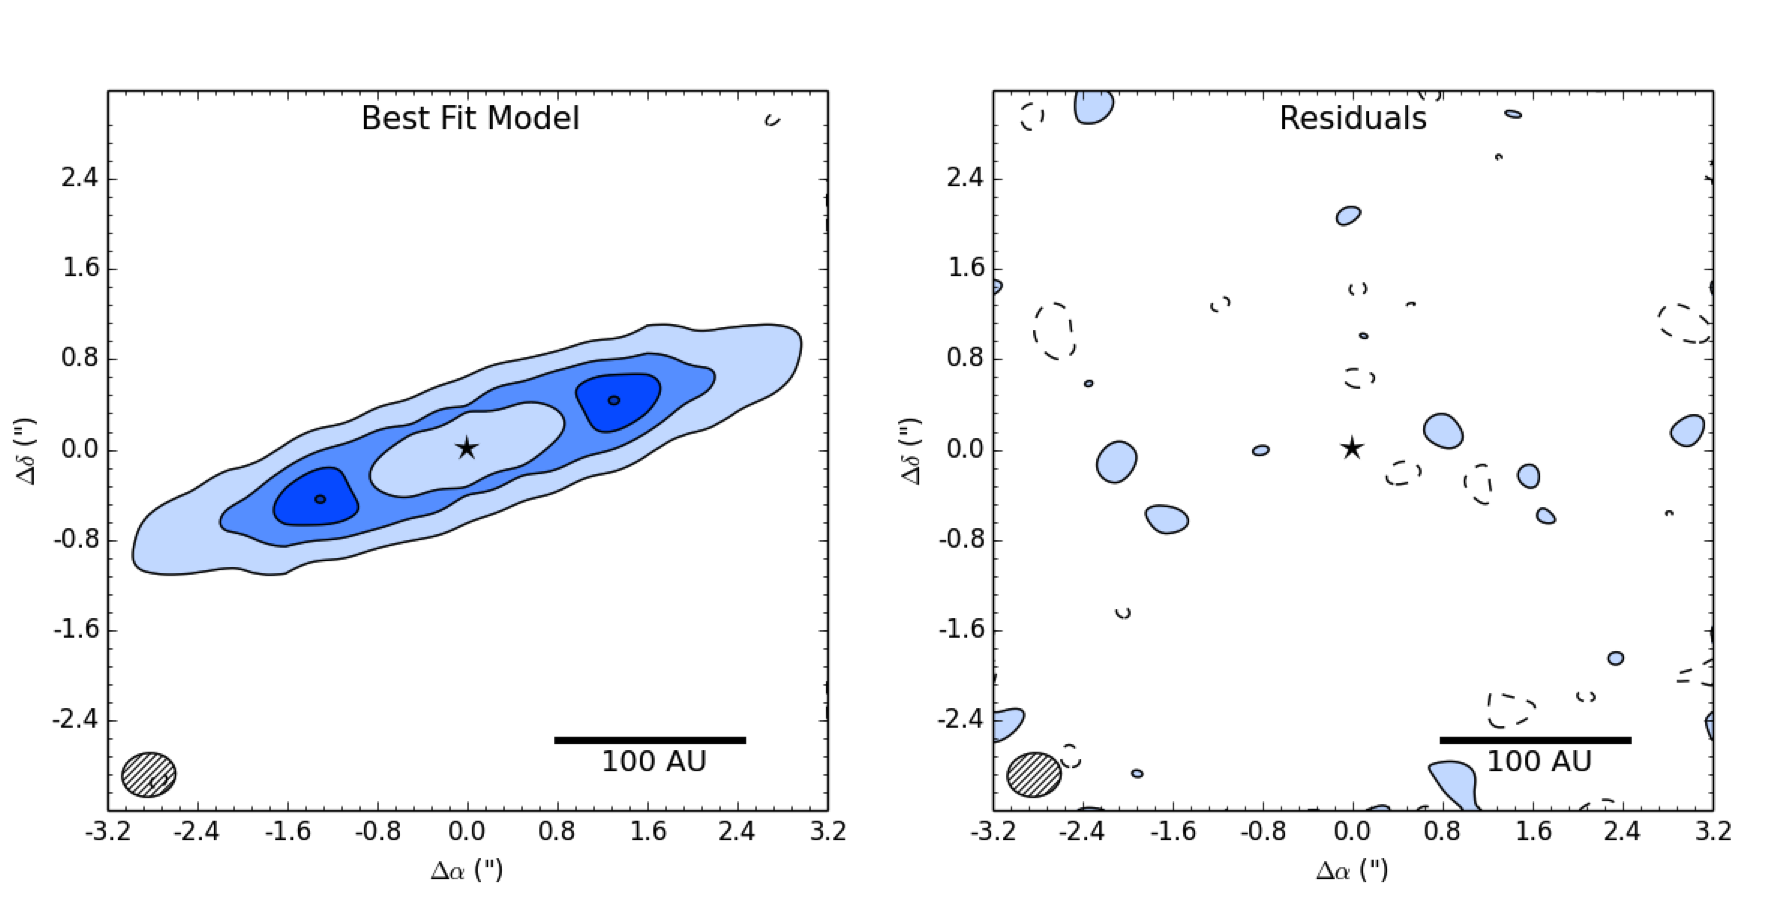
\includegraphics[width = 1\textwidth]{49CET_nOBAG_ModelResidual.png}
\caption{The model image (left) and residuals (right) for the single power law model with two characteristic grain sizes. Contours are [-2, 2, 4, 6, 8] $\times$ 58$\,\mu$Jy.}
\label{fig:49CET_nOBAG_ModelResidual}
\end{figure}

Given the success of the single power law description of the surface density fitting just the visibilities but the discrepancies introduced in a simultaneous fit, we propose an inner disk of grains, with a different characterization of the surface density, is necessary to recreate the mid-IR excess. Building upon the results of \cite{Wahh07}, who resolved the inner disk of small grains and had a best fit model that specified $a$ = 0.1$\,\mu m$, we described an inner disk with a grain size of 0.1$\,\mu m$ from $R_{In}$ to $R_{Inner Disk}$ with $\Sigma_{Inner Disk} \propto r^{-1}$, and vary all the parameters described by Equation \ref{eq:sigma100} as an outer belt, which extends from $R_{Inner Disk}$ to $R_{Out}$. The outer radius of the disk is modeled as $R_{In}$ + $\Delta R$. Because small grains radiate at higher temperatures at a given distance from the star than their larger brethren as described by \ref{eq:fullEBalance}, they were able to boost the mid-IR flux without contributing significantly to the flux at millimeter wavelengths.


\begin{figure}%[!]
\centering
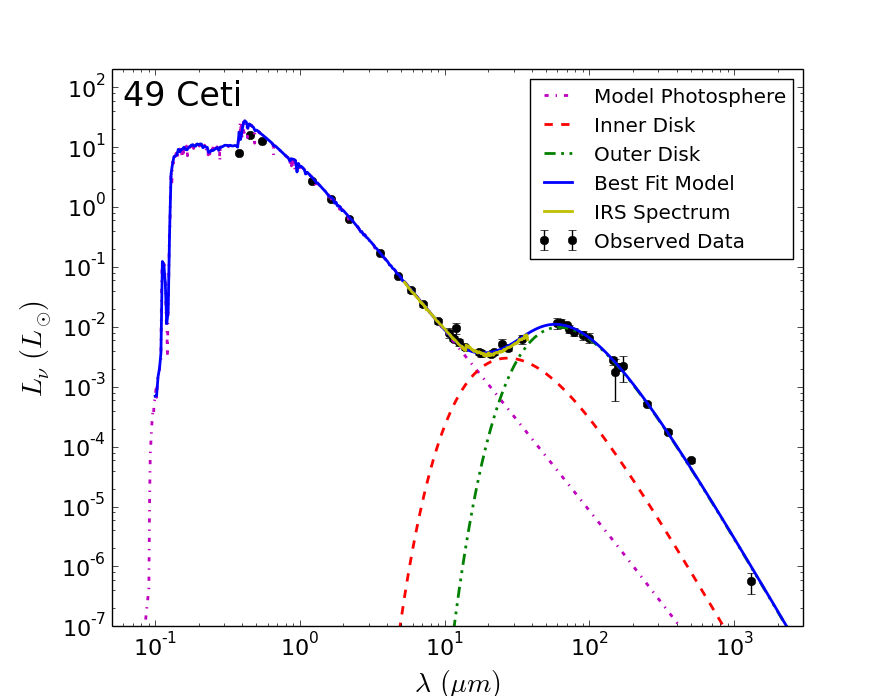
\includegraphics[width = 1\textwidth]{49CET_nOBAG_SED.png}
\caption{The best fit SED of 49 Ceti for the single power law model simultaneously fitting the SED and visibilities with two characteristic grain sizes. The best fit model is the sum of the inner disk model, outer disk model, and the model photosphere.}
\label{fig:49CET_nOBAG_SED}
\end{figure}

\begin{table}
\begin{center}
    \def\arraystretch{1.1}%
    \begin{tabular}{l*{2}{c}r}
    \hline
    Parameter & Median Value $\pm$ 1$\sigma$ & Best Fit Value \\ \hline
     $R_{In}$  [AU] & 5$^{+2}_{-1}$ & 6\\  
     $R_{Inner Disk}$ [AU] & 73$^{+3}_{-3}$ & 73\\      
     $\Delta R$ [AU] & 310$^{+9}_{-9}$ & 310\\ 
     log($M_{Outer Disk}$ [$M_{\oplus}$]) & -1.17$^{+0.08}_{-0.10}$ & -1.16 \\
     log($M_{Inner Disk}$ [$M_{M_{\oplus}}$]) & -3.1$^{+0.2}_{-0.2}$ & -3.0 \\     
     log(a [$\mu$m]) & 0.08$^{+0.11}_{-0.14}$ & 0.09\\ 
     $\beta$ & 1.17$^{+0.05}_{-0.05}$ & 1.18\\ 
     $p$ & 1.29$^{+0.11}_{-0.11}$ & 1.27\\ 
     $i$ [$^\circ$] & 79.4$^{+0.4}_{-0.4}$ & 79.3 \\ 
     $PA$ [$^\circ$] & -71.4$^{+0.4}_{-0.5}$ & -71.3\\
    \hline
    \end{tabular}
\end{center}
\caption{The median and best fit values for the single power law model with two characteristic grain sizes simultaneously fitting the SED and visibilities.}
\label{tab:49CET_nOBAG_Table}
%for all parameters of the model of 49 Ceti's dust disk. THIS IS SIMPLE BONUS BELT, JUST VIS100x840}
\end{table}


%%%%%%%

\section{The Unresolved Surface Density Enhancement (USDE)}
\label{USDE}

\subsection{Visibility-only Fit}
\label{USDE_Vis}

\begin{figure}[t!]
\centering
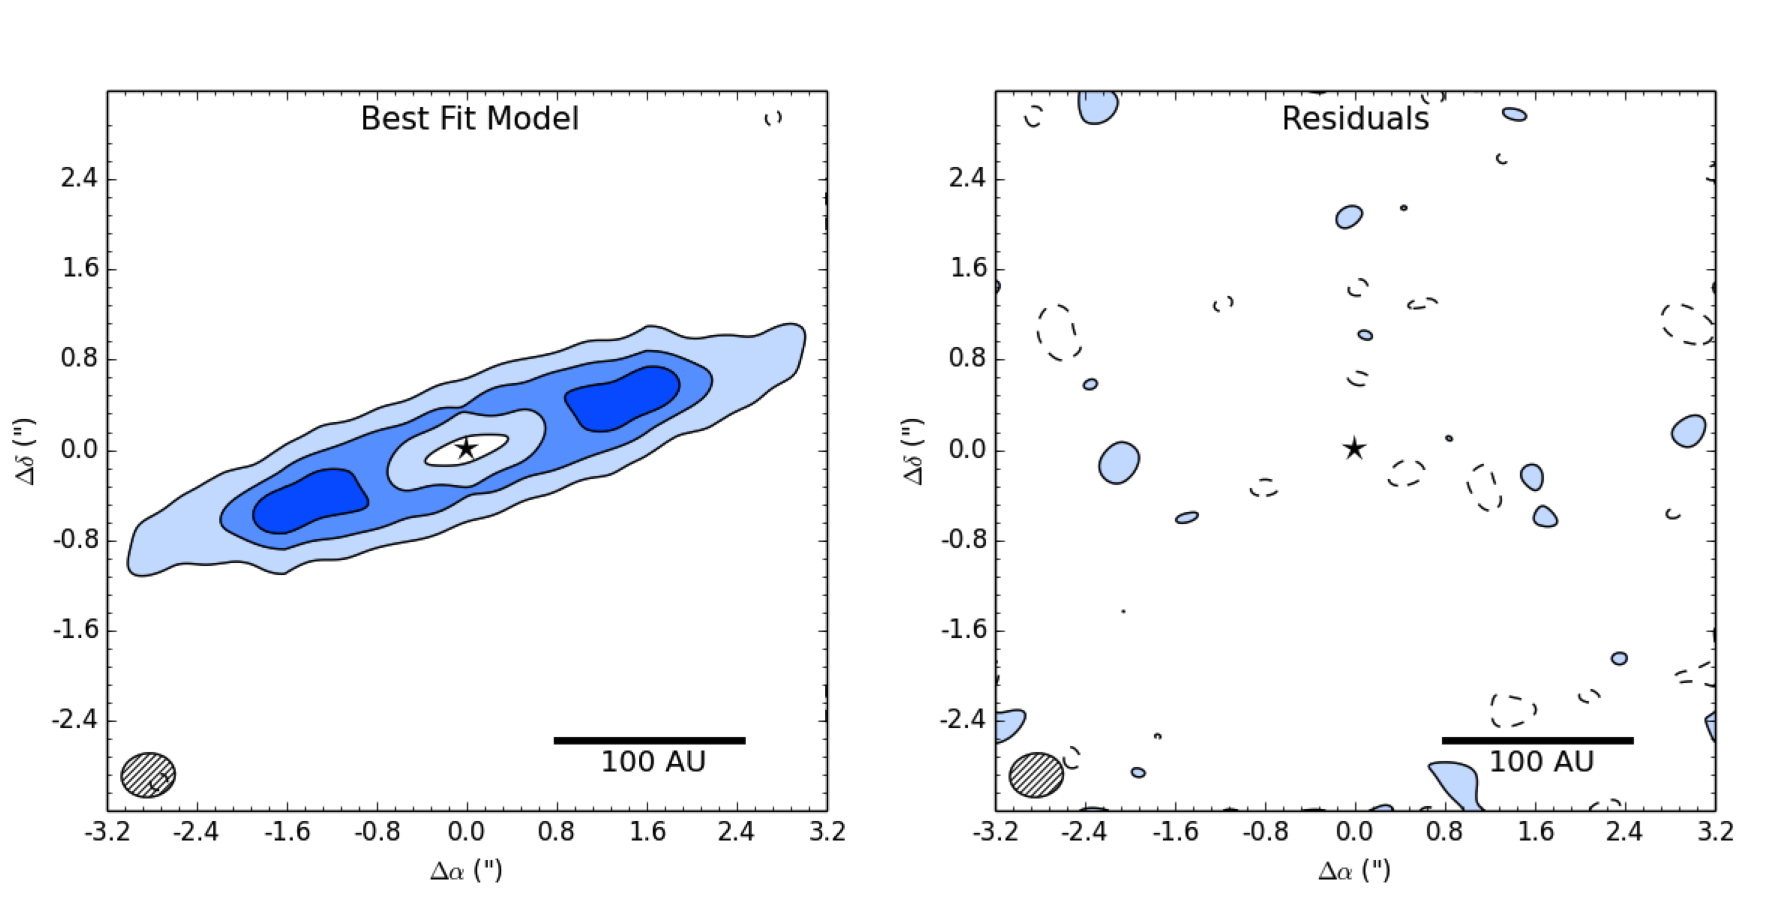
\includegraphics[width = 1\textwidth]{49CET_BonusBeltVIS_ModelResidual.png}
\caption{The model image (left) and residuals (right) for the unresolved surface density enhancement model fitting just the visibilities. Contours are [-2, 2, 4, 6] $\times$ 58$\,\mu$Jy. The model leaves only a small scatter of 2$\sigma$ residuals.}
\label{fig:49CET_BonusBeltVIS_ModelResidual}
\end{figure}

Although the single power law description of the surface density adequately describes the data, the ring-like structure apparent at $\sim$ 100\,AU in the data image suggests a ring-like description of the surface density in our model could provide a better fit. To do this, we add a narrow, spatially unresolved belt, which we model to be 3\,AU wide at a distance $R_{Belt}$ and of mass $M_{Belt}$, on top of of the single power law description of the surface density that extends from $R_{In}$ to $R_{Out}$ as described in Section \ref{SinglePowerSED_Model}. 

As can be seen in the best-fit model and residual images displayed in Figure \ref{fig:49CET_BonusBeltVIS_ModelResidual}, this USDE model does a very good job of recreating the visibilities, and the residual image seems identical to that of the single power law visibility-only fit (see Section \ref{stats} for the statistical analysis of the comparison between these fits). Both models show evidence for an inner disk that is devoid of large grains, as the best-fit inner radius of 56\,AU derived in this model is close to the value of 69\,AU derived in the single power law visibility-only fit (see Table \ref{tab:49CET_BonusBeltVIS_Table} for all parameters derived from the MCMC chain for this model). 


%However, 49 Ceti seems to show a ring-like structure at $\sim$ 100 AU, suggesting a more complex model of the surface density could provide a better fit. A simple power law with a narrow density enhancement to mimic this ``ring" is described in Section ??<<??, and a double power law, with surface density increasing to the radius of this ``ring" before decreasing, is presented in Section ??<<??????. 

%The ring-like positive residuals left by the single power law model suggest the need for a more complex model of the surface density. We propose a double power law model in which the surface density increases from $R_{In}$ to a transition radius $R_{T}$ before dropping off until $R_{Out}$ in section \ref{DoublePowerSED_Model} and a single power law with a narrow, unresolved surface density enhancement in section \ref{UnresolvedDensitySED_Model}.

%Unlike the double power law model, fitting to just the visibilities with the best-fit unresolved density enhancement model resolves the inner radius of the disk to be 56AU (See Table \ref{tab:49CET_BonusBeltVIS_Table}), whereas the double power law model settled on a best-fit of 6AU. This larger value for $R_{In}$ is visible in the best-fit model image (Figure \ref{fig:49CET_BonusBeltVIS_ModelResidual}), as there is no emission next to the star. However, this difference has no significant effect on the residual image map, which shows basically the same scatter of -2$\sigma$ residuals as in the double power law best-fit residual image. 

%To see how strongly the SED was altering the best-fit models, we ran fits with MCMC based just on the visibility $\chi^{2}$. We find that both the double power law and unresolved surface density enhancement models are able to recreate the visibilities, and that differences between parameters between the two models are not significant. This is clear both from the minimal leftovers in each residual image and from an F-test, which confirmed that neither model is better the other in a statistically significant way.

%Both models settle on approximately the same radius for the peak of the surface density. $R_{T}$ = 105AU for the double power law model, and $R_{Belt}$ = 113AU for the unresolved surface density enhancement model. Without the simultaneous fit to the SED, $M_{Disk}$, $\beta$, and $a$ are not well constrained.

\begin{table}
\begin{center}
    \def\arraystretch{1.37}%
    \begin{tabular}{l*{2}{c}r}
    \hline
    Parameter & Median Value $\pm$ 1$\sigma$ & Best Fit Value \\ \hline
     $R_{In}$  [AU] & 58$^{+6}_{-6}$ & 56\\  
     $\Delta R$ [AU] & 248$^{+8}_{-8}$ & 252\\ 
     log($M_{Disk}$ [$M_{\oplus}$]) & -0.8$^{+0.5}_{-0.9}$ & -0.7 \\
     $R_{Belt}$  [AU] & 114$^{+3}_{-3}$ & 113\\ 
     log($M_{Belt}$ [$M_{\oplus}$]) & -1.9$^{+0.6}_{-0.8}$ & -1.6\\
     log(a [$\mu$m]) & 0.3$^{+0.9}_{-0.7}$ & -0.1\\ 
     $\beta$ & 1.4$^{+0.4}_{-0.4}$ & 1.4\\ 
     $p$ & 0.6$^{+0.4}_{-0.4}$ & 0.6\\ 
     $i$ [$^\circ$] & 79.4$^{+0.4}_{-0.4}$ & 79.4 \\ 
     $PA$ [$^\circ$] & -71.2$^{+0.4}_{-0.6}$ & -71.1\\
    \hline
    \end{tabular}
\end{center}
\caption{The median and best fit values for the unresolved density enhancement model fitting only the visibilities.}
\label{tab:49CET_BonusBeltVIS_Table}
%for all parameters of the model of 49 Ceti's dust disk. THIS IS SIMPLE BONUS BELT, JUST VIS100x840}
\end{table}


\subsection{Simultaneous SED and Visibility Fit}

Simultaneously fitting the USDE model to the SED and visibilities comes close to recreating both the images and the visibilities, but runs into similar issues that the single power law model of Section \ref{Simple_SED_Vis} encountered. The sum of the fluxes from the model photosphere, broad power law disk, and narrow ring is displayed in Figure \ref{fig:49CET_BonusBeltSED_SED} and is a good fit to the photometric data. While the IR excess is dominated by the disk model, the belt contributes a non-negligible flux to the SED, both at the IR excess peak of $\sim$ 70$\,\mu m$ and at the wavelength of the ALMA image (850$\,\mu m$). 

\begin{figure}%[t!]
\label{fig:49CET_BonusBeltSED_SED}
\centering
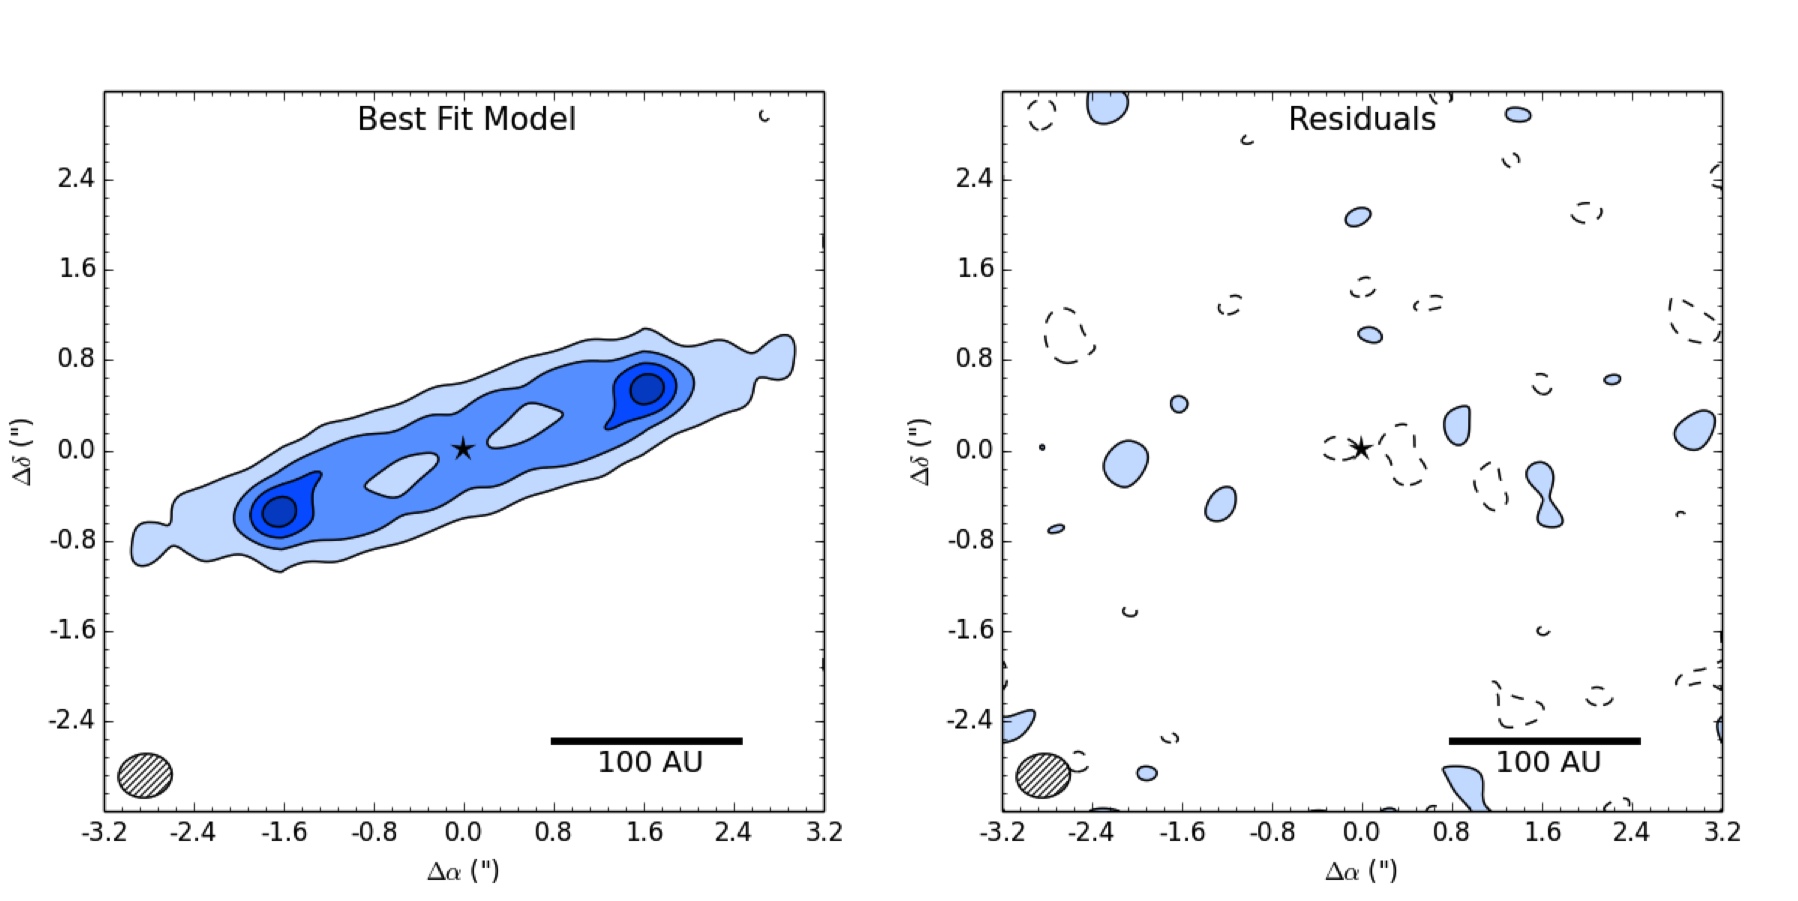
\includegraphics[width = 1\textwidth]{49CET_BonusBeltSED_ModelResidual.png}
\caption{The model image (left) and residuals (right) for the unresolved surface density enhancement model, simultaneously fitting the SED and the visibilities. Contours are [-2, 2, 4, 6, 8] $\times$ 58$\,\mu$Jy. The model successfully takes care of the region of high density on the southeast side of the disk, but is still slightly too bright at the center.}
\label{fig:49CET_BonusBeltSED_ModelResidual}
\end{figure}

\begin{figure}%[H]
\centering
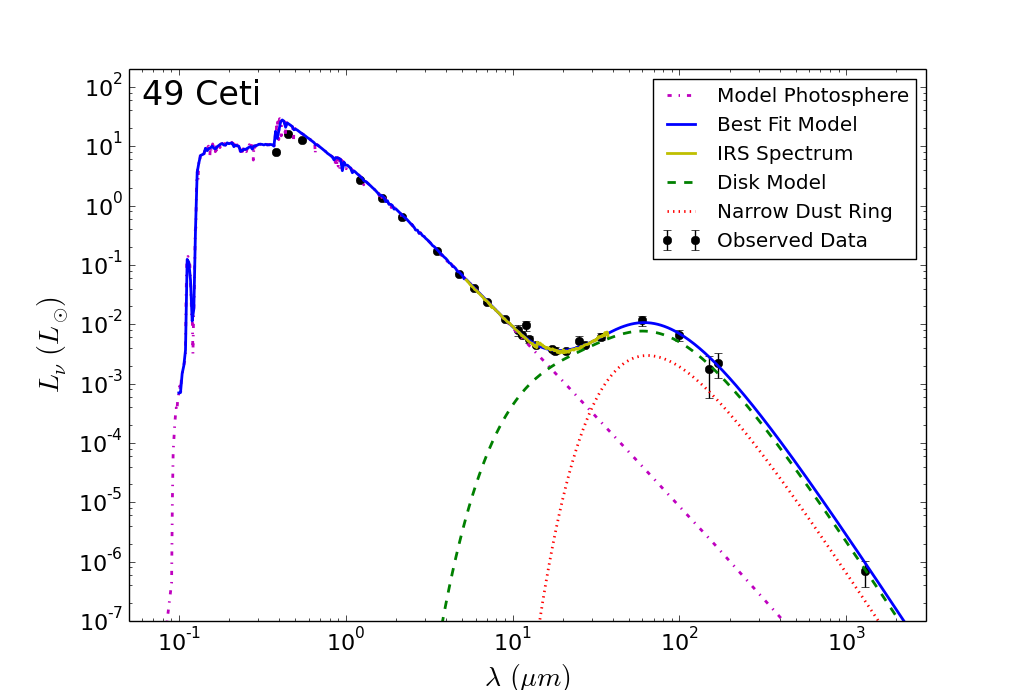
\includegraphics[width = 1\textwidth]{49CET_BonusBeltSED_SED.png}
\caption{The best fit SED of 49 Ceti for the unresolved surface density enhancement model. The best fit model is the sum of the disk model, the model photosphere, and the narrow dust ring.}
\label{fig:49CET_BonusBeltSED_SED}
\end{figure}

\begin{table}
\begin{center}
    \def\arraystretch{1.2}%
    \begin{tabular}{l*{2}{c}r}
    \hline
    Parameter & Median Value $\pm$ 1$\sigma$ & Best Fit Value \\ \hline
     $R_{In}$  [AU] & 1.3$^{+0.7}_{-0.5}$ & 1.3\\  
     $\Delta R$ [AU] & 290$^{+8}_{-7}$ & 291\\ 
     log($M_{Disk}$ [$M_{\oplus}$]) & -1.1$^{+0.2}_{-0.2}$ & -1.1 \\
     $R_{Belt}$  [AU] & 112$^{+2}_{-2}$ & 112\\ 
     log($M_{Belt}$ [$M_{\oplus}$]) & -1.8$^{+0.2}_{-0.2}$ & -1.7\\
     log(a [$\mu$m]) & 0.27$^{+0.17}_{-0.19}$ & 0.31\\ 
     $\beta$ & 1.25$^{+0.15}_{-0.12}$ & 1.27\\ 
     $p$ & -0.11$^{+0.06}_{-0.06}$ & -0.07\\ 
     $i$ [$^\circ$] & 79.5$^{+0.4}_{-0.4}$ & 79.5 \\ 
     $PA$ [$^\circ$] & -71.0$^{+0.4}_{-0.4}$ & -71.0\\
    \hline
    \end{tabular}
\end{center}
\caption{The median and best fit values for the unresolved density enhancement model fitting the SED and visibilities.}
%for all parameters of the model of 49 Ceti's dust disk. THIS IS SIMPLE BONUS BELT, VIS & SED 120x842 WITH CORRECT UNCERTAINTIES}
\label{tab:49CET_BonusBeltSED_Table}
\end{table}

However, the simultaneous best-fit USDE model has $R_{In}$ = 1.3\,AU in order to generate enough hot grains to recreate the mid-IR excess of the SED, and with just one characteristic grain size ($a \sim 2\,\mu m$), the inner disk contributes too much flux at the wavelength of the ALMA image. This results in more in negative residuals than were apparent in the visibility-only fit at the center of the best-fit residual image as can be seen in Figure \ref{fig:49CET_BonusBeltSED_ModelResidual}. This model suggests a surface density that increases slightly with radius ($p$ = $-0.07$), but the visibility-only fit found $p$ = 0.6, showing that the SED's influence is resulting in an inferior fit to the visibilities. Because of the addition of the unresolved density enhancement, this model does better at accounting for the ring-like residuals that were left behind by the single power law model with one characteristic grain size, but as with the single power law, the discrepancy between the visibility-only fit and the simultaneous fit necessitates a disk model with two characteristic grain sizes. 


%The best-fit model and residuals are displayed in Figure \ref{fig:49CET_BonusBeltSED_ModelResidual}, and the table of values derived from the MCMC chain is presented in Table \ref{tab:49CET_BonusBeltSED_Table}. The best-fit SED is shown in Figure \ref{fig:49CET_BonusBeltSED_SED}, with separate contributions to the total flux of the model displayed for the broad disk described by the single power law and by the additional belt. 

%The total best-fit mass for this model is 0.10 $M_{\oplus}$, whereas the simple power law model had a mass of 0.23$M_{\oplus}$
%The best-fit value of $p$ shows that the disk is nearly flat, whereas
%This model does a better job at recreating the density enhancement in the disk and still fitting to the SED, but just like with the double power law model, it is too bright at the center. As earlier, in order to create grains hot enough to boost the mid-IR flux with only one characteristic grain size population, the inner radius of the disk is pushed inward to ~1AU. These grains are then able to recreate the mid-IR excess, but in doing so contribute too much flux at the wavelength of the ALMA image, resulting in a model that is too bright near the star.

\subsection{Simultaneous SED and Visibility Fit with Two Characteristic Grain Sizes}

\begin{figure}[t!]
\centering
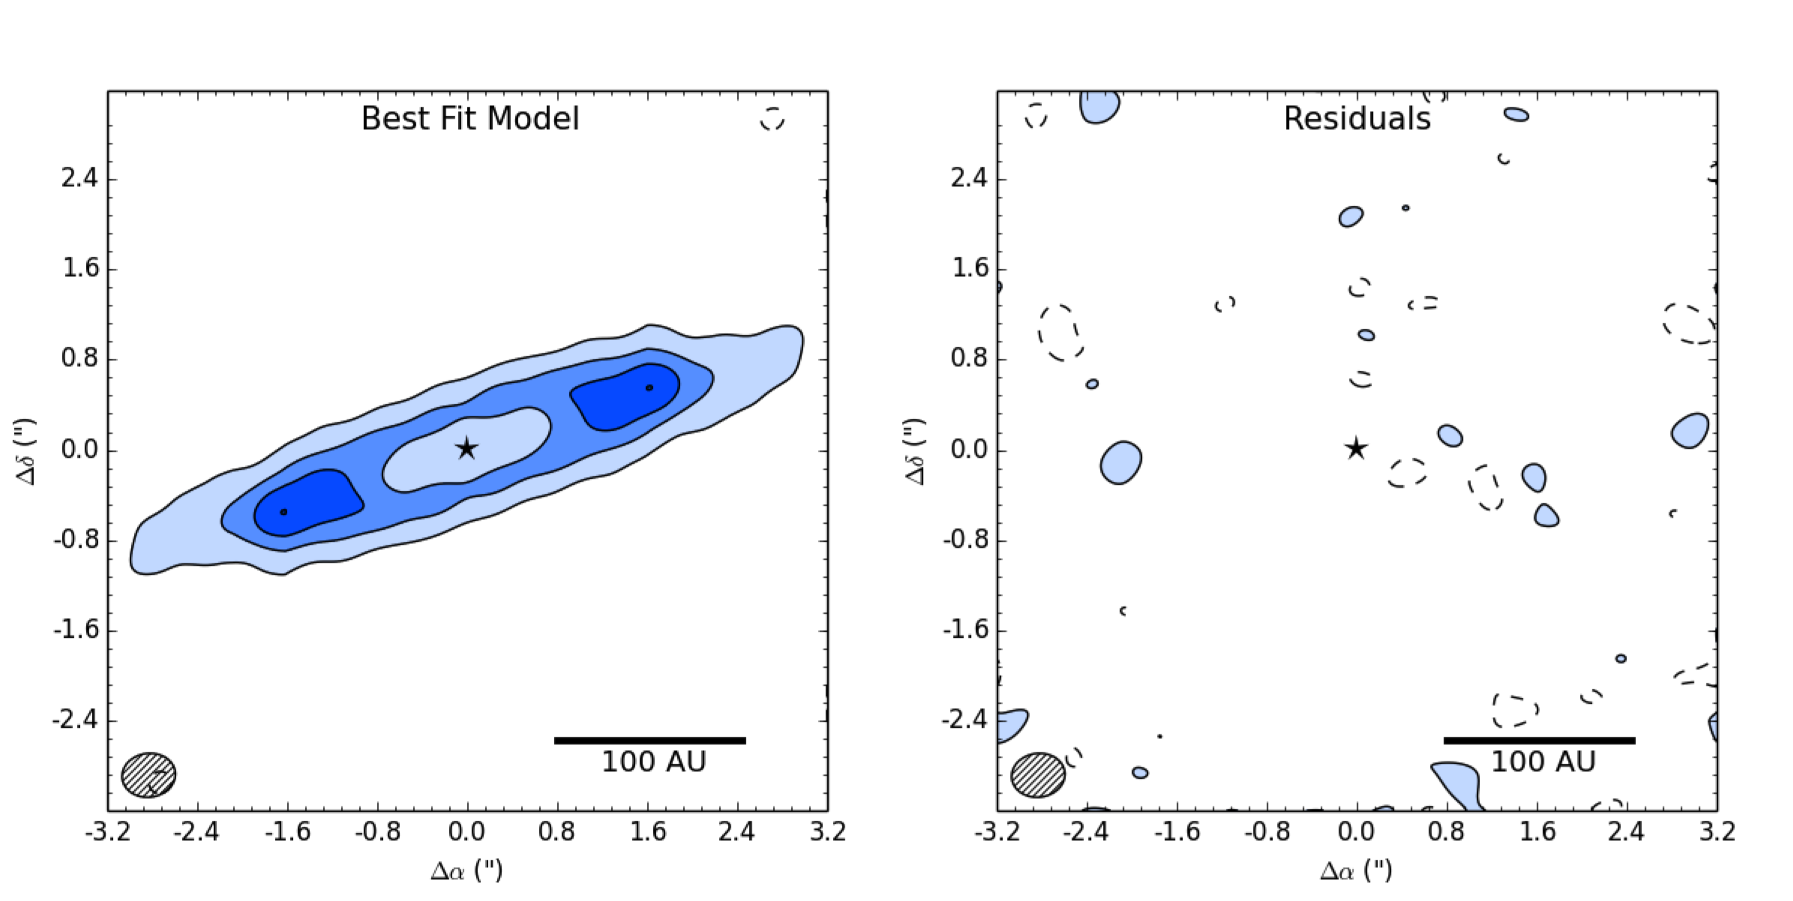
\includegraphics[width = 1\textwidth]{49CET_bBBAG_ModelResidual.png}
\caption{The model image (left) and residuals (right) for the USDE model with an an additional inner disk of small grains. Contours are [-2, 2, 4, 6, 8] $\times$ 58$\,\mu$Jy. The model leaves only a small scatter of 2$\sigma$ residuals.}
\label{fig:49CET_bBBAG_ModelResidual}
\end{figure}
\end{table}

As earlier, we implement an inner disk of 0.1$\,\mu m$ grains from $R_{In}$ to $R_{Inner Disk}$ with $\Sigma_{Inner Disk} \propto r^{-1}$ to complement the outer disk with the additional surface density enhancement described above. This model is able to simultaneously fit the SED (not displayed) without it significantly influencing the best-fit parameters derived from the USDE visibility-only fit (Section \ref{USDE_Vis}). For example, the best-fit value of $p$ derived in the USDE model with two characteristic grain sizes is 0.75, which is statistically equivalent to that of the USDE visibility-only best-fit value within our uncertainties (see Table \ref{tab:bBBAG_Table}). Both this model and the single power law with two characteristic grain sizes settle on $R_{Inner Disk} \sim$ 70\,AU, providing further evidence that there is a clear turnover around this radius of an inner disk of small grains and an outer disk of larger grains. The best-fit model and residuals are displayed in Figure \ref{fig:49CET_bBBAG_ModelResidual} and look very similar to those of the single power law model with two characteristic grain sizes, though the peak of $8\sigma$ emission apparent in this model is farther out than in the other model, a result of the surface density peaking at $\sim$ 114\,AU rather than $\sim$ 73\,AU. 

\begin{figure}%[t!]
\label{fig:49CET_USDE_TWO_SED}
\centering
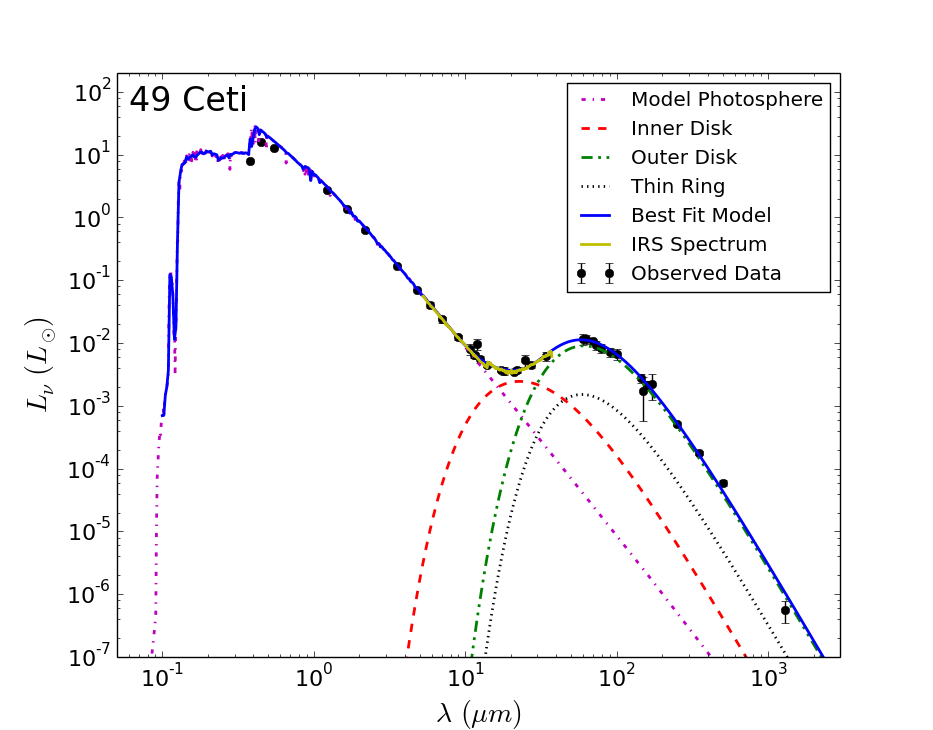
\includegraphics[width = \textwidth]{49CET_bBBAG_SED.png}
\caption{The SED for the USDE model fitting the SED and visibilities for the two part disk model. The best fit model is the sum of the inner disk, outer disk, narrow ring, and model photosphere. }
\label{fig:49CET_BonusBeltSED_ModelResidual}
\end{figure}



\begin{table}
\begin{center}
    \def\arraystretch{1.2}%
    \begin{tabular}{l*{2}{c}r}
    \hline
    Parameter & Median Value $\pm$ 1$\sigma$ & Best Fit Value \\ \hline
     $R_{In}$  [AU] & 4.6$^{+1.5}_{-1.2}$ & 3.5\\  
     $\Delta R_{Out}$ [AU] & 302$^{+9}_{-8}$ & 303\\ 
     $R_{Inner Disk}$ [AU] & 62$^{+5}_{-5}$ & 60\\ 
     $R_{Ring}$  [AU] & 114$^{+3}_{-3}$ & 114\\ 
     log($M_{Inner Disk}$ [$M_{\oplus}$]) & -3.3$^{+0.2}_{-0.2}$ & -3.4 \\
     log($M_{Outer Disk}$ [$M_{\oplus}$]) & -1.21$^{+0.09}_{-0.10}$ &-1.21 \\
     log($M_{Ring}$ [$M_{\oplus}$]) & -2.26$^{+0.15}_{-0.18}$ &-2.26 \\
     log(a [$\mu$m]) & 0.09$^{+0.10}_{-0.13}$ & 0.06\\ 
     $\beta$ & 1.17$^{+0.05}_{-0.05}$ & 1.17\\ 
     $p$ & 0.80$^{+0.19}_{-0.17}$ & 0.75\\ 
     $i$ [$^\circ$] & 79.3$^{+0.4}_{-0.4}$ & 79.3 \\ 
     $PA$ [$^\circ$] & -71.4$^{+0.4}_{-0.4}$ & -71.2\\
    \hline
    \end{tabular}
\end{center}
\caption{Parameters derived from the MCMC chain for the USDE model with two characteristic grain sizes.}
\label{tab:bBBAG_Table}
\end{table}


%%%%%%%%%%%%%%%%%%%%%%%%%

\section{The Double Power Law}
\label{DP}

Another means of describing a ring-like structure is with a double power law that increases in surface density to a variable radius before dropping off. This model, which has the same number of free parameters as the USDE model, provides a comparison for us to discern whether or not the surface density enhancement is resolved in our data. We parameterize $\Sigma(r)$ for the double power law normalized to the surface density at the transition radius, $\Sigma_{T}$. We model the transition radius, $R_{T}$ as $R_{In} + \Delta R_{T}$, and the outer radius, $R_{Out}$, as $R_{In} + \Delta R_{T} + \Delta R_{Out}$.

\begin{equation}\label{eq:sigmaDP}
\Sigma(r) = \begin{cases}
   \Sigma_{T}\Big(\frac{r}{R_{T}}\Big)^{-p_{1}} & \text{for $R_{In}$ $\le$ r $\le R_{T}$} \\
   \Sigma_{T}\Big(\frac{r}{R_{T}}\Big)^{-p_{2}} & \text{for $R_{T}$ $\textless$ r $\le$ $R_{Out}$}
\end{cases}
\end{equation}

As earlier, we solve for $M_{Disk}$:

\begin{equation}\label{eq:mdiskDP}
\begin{flalign*}
    M_{Disk} &= \int_{R_{In}}^{R_{T}} \Sigma(r) 2 \pi r \,dr & \\
    &= \int_{R_{In}}^{R_{T}} \Sigma_{\text{T}}\Big(\frac{r}{R_{T}}\Big)^{-p_{1}} 2 \pi r \,dr & + \int_{R_{T}}^{R_{Out}} \Sigma_{\text{T}}\Big(\frac{r}{R_{T}}\Big)^{-p_{2}} 2 \pi r \,dr &&
\end{flalign*}
\end{equation}

We integrate and solve for $\Sigma_{T}$, defining $j_{1} = 2 - p_{1}$, $j_{2} = 2 - p_{2}$, $m_{1} = R_{T}^{j_{1}} - R_{In}^{j_{1}$, and $m_{2} = R_{Out}^{j_{2}} - R_{T}^{j_{2}$ for readability:

\begin{equation}\label{eq:sigmaT}
\Sigma_{T} = \cfrac{M_{Disk} (j_{1} j_{2})}{2\pi [(m_{1} j_{2})(R_{T})^{p_{1}} + (m_{2} j_{1})(R_{T})^{p_{2}}]}
\end{equation}

This parameterization of $\Sigma_{T}$ allows us to vary $R_{In}$, $R_{T}$, $R_{Out}$, $M_{Disk}$, $p_{1}$, and $p_2$ in our search for a best-fit model. We use $a$ and $\beta$ to describe the population of grains and $i$ and $PA$ to describe the geometry on the sky as in the single power law model. 

\subsection{Visibility-only Fit}

\begin{figure}
\centering
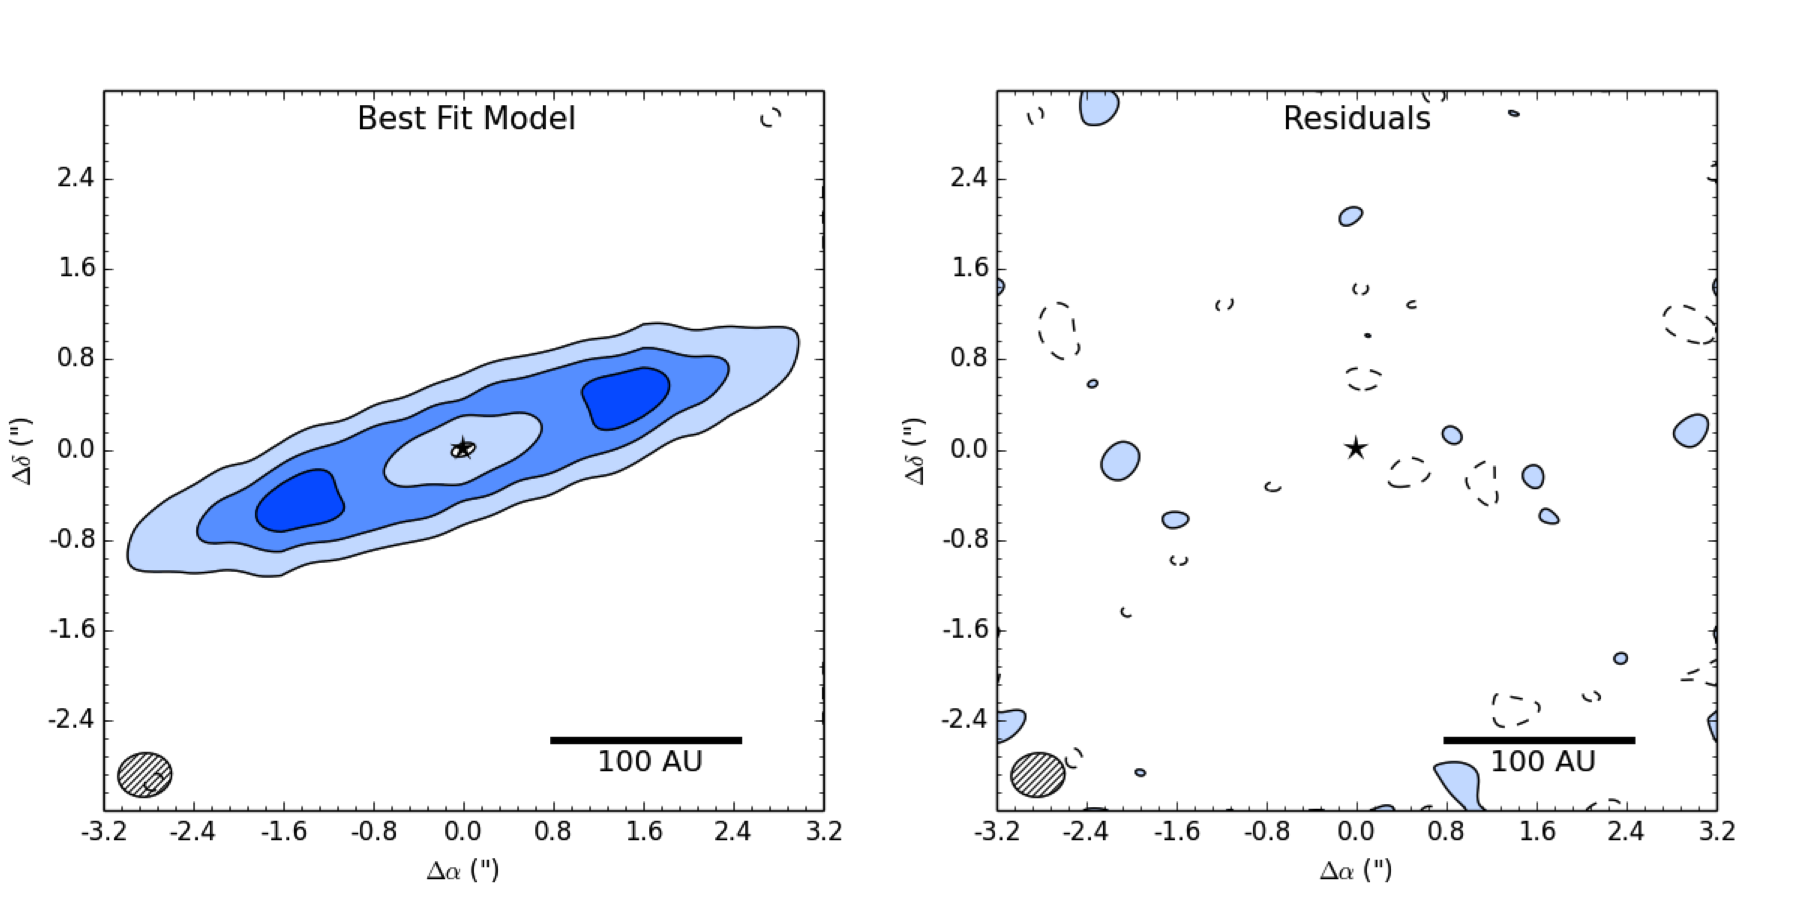
\includegraphics[width = 1\textwidth]{49CET_DoublePowerVIS_ModelResidual.png}
\caption{The model image (left) and residuals (right) for the double power law model fitting just the visibilities. Contours are [-2, 2, 4, 6] $\times$ 58$\,\mu$Jy. The model leaves only a small scatter of 2$\sigma$ residuals.}
\label{fig:49CET_DoublePowerVIS_ModelResidual}
\end{figure}

\begin{table}
\begin{center}
    \def\arraystretch{1.37}%
    \begin{tabular}{l*{2}{c}r}
    \hline
    Parameter & Median Value $\pm$ 1$\sigma$ & Best Fit Value \\ \hline
     $R_{In}$  [AU] & 26$^{+20}_{-17}$ & 6\\  
     $\Delta R_{T}$ [AU] & 78$^{+16}_{-17}$ & 99\\ 
     $\Delta R_{Out}$ [AU] & 215$^{+13}_{-12}$ & 212\\ 
     log($M_{Disk}$ [$M_{\oplus}$]) & -1.4$^{+0.5}_{-0.5}$ & -2.2 \\
     log(a [$\mu$m]) & 0.5$^{+0.4}_{-0.4}$ & 0.4\\ 
     $\beta$ & 1.4$^{+0.3}_{-0.3}$ & 0.8\\ 
     $p1$ & -1.7$^{+0.6}_{-0.6}$ & -1.8\\ 
     $p2$ & 1.52$^{+0.19}_{-0.16}$ & 1.55\\ 
     $i$ [$^\circ$] & 79.2$^{+0.4}_{-0.4}$ & 79.1 \\ 
     $PA$ [$^\circ$] & -71.7$^{+0.5}_{-0.5}$ & -71.5\\
    \hline
    \end{tabular}
\end{center}
\caption{The median and best fit values for the double power law model fitting only the visibilities.}
% for all parameters of the model of 49 Ceti's dust disk, THIS IS DOUBLE POWER VIS ONLY 100x600}
\label{tab:49CET_DoublePowerVIS_Table}
\end{table}

Fitting to just the visibilities with the double power law model adequately describes the data, as can be seen by the lack of significant residuals in Figure \ref{fig:49CET_DoublePowerVIS_ModelResidual}. The values derived from the MCMC chain are displayed in Table \ref{tab:49CET_DoublePowerVIS_Table}. Although the best-fit inner radius of this model is still close to the star ($\sim$ 6\,AU), it ramps up toward $R_{T}$ quite steeply ($\Sigma_{Inner Disk} \propto r^{1.8}$) and doesn't result in any systematic -2$\sigma$ residuals near the star. In addition, not under the influence of the SED, it is able to recreate the region of higher density. 

\subsection{Simultaneous SED and Visibility Fit}

\begin{figure}
\centering
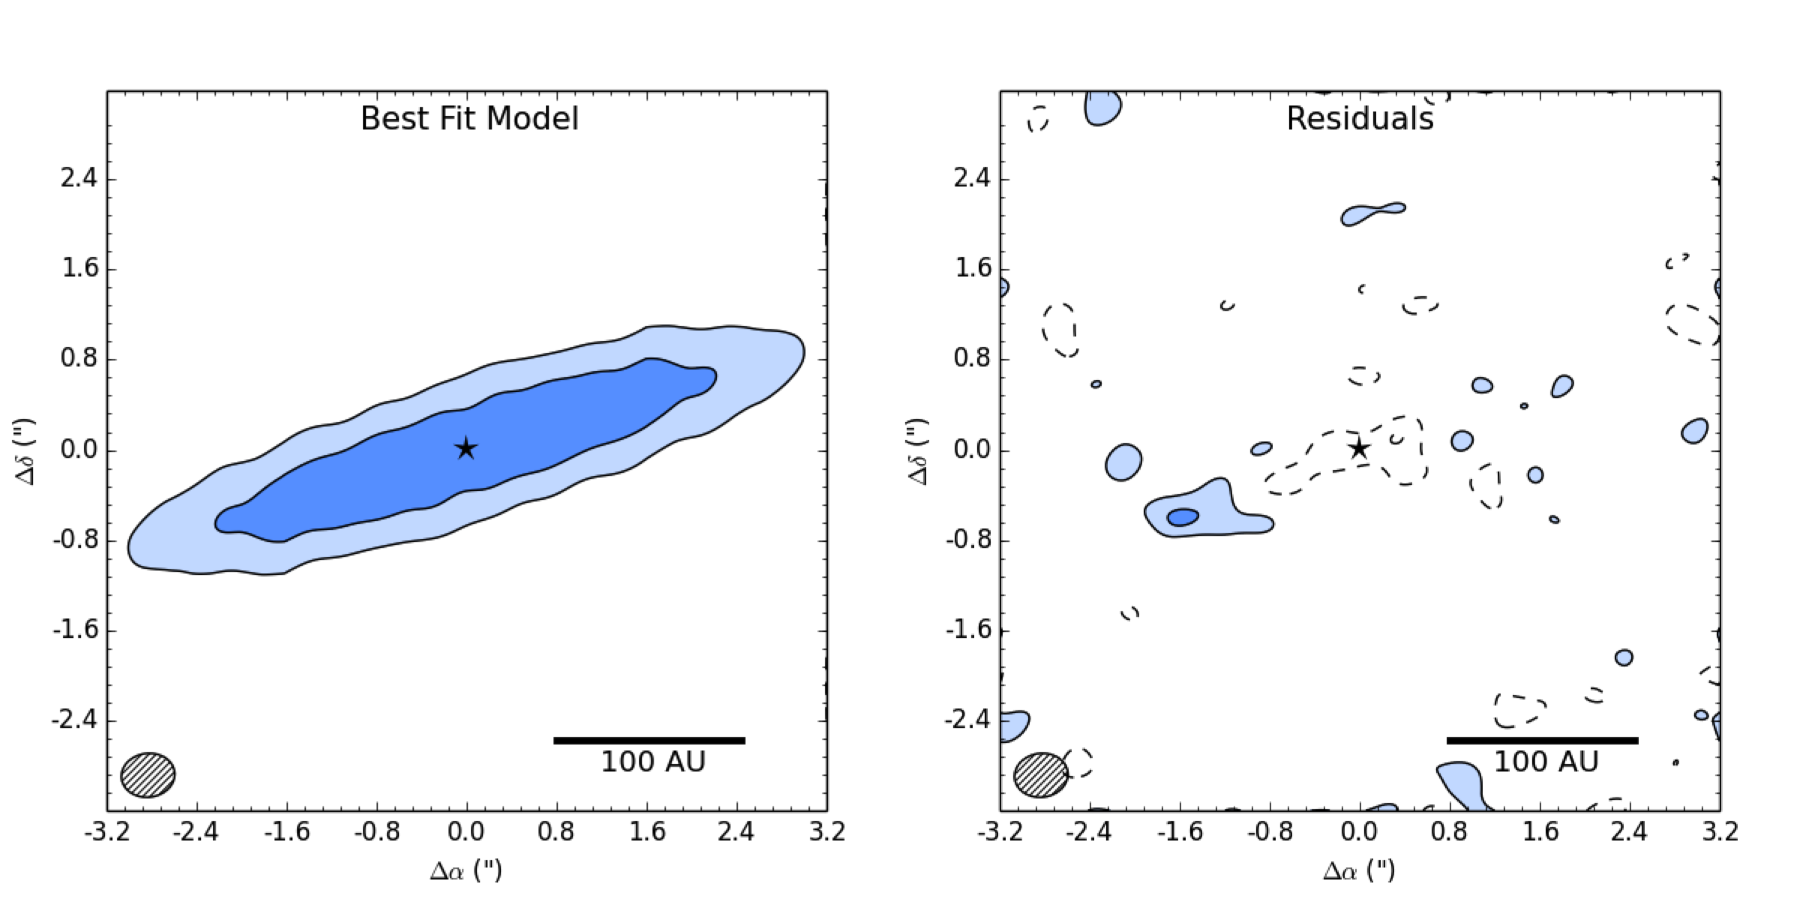
\includegraphics[width = 1\textwidth]{49CET_DoublePowerSED_ModelResidual.png}
\caption{The model image (left) and residuals (right) for the double power law model, simultaneously fitting the SED and the visibilities. Contours are [-4, -2, 2, 4] $\times$ 58$\,\mu$Jy.}
\label{fig:49CET_DoublePowerSED_ModelResidual}
\end{figure}

Values derived from the MCMC chain for the double power law model simultaneously fitting to the SED and visibilities are presented in Table \ref{tab:doublePowerSEDTable}, and the best-fit model and corresponding residuals are displayed in Figure \ref{fig:49CET_DoublePowerSED_ModelResidual}. This model returned a best-fit value for $p_{1}$ of $-$0.25, which is significantly different from that derived in the visibility-only fit ($p_{1} = -1.8$), resulting in a disk model that is too bright at small radii. In addition, the model was unable to account for the region of higher density on the southeast side apparent in the resolved ALMA data, even though it was able to in the visibility-only fit. As with earlier simultaneous fits with just one characteristic grain size, these effects are the result of the fit to the SED (Figure \ref{fig:49CET_DP_SED}). 

\begin{figure}%[t!]
\label{fig:49CET_DP_SED}
\centering
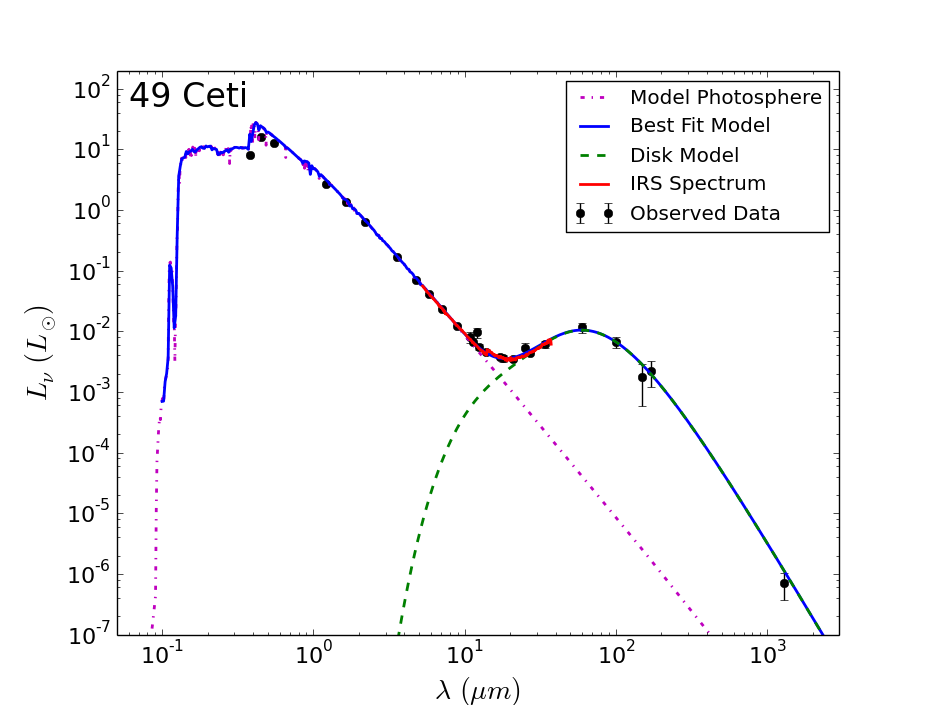
\includegraphics[width = 1\textwidth]{49CET_DP_SED.png}
\caption{The SED for the double power law model fitting the SED and visibilities for the disk model with just one characteristic grain size. }
\label{fig:49CET_DP_SED}
\end{figure}

%In addition, it is brighter at the center of the disk than even the simple power law model, as can be seen from the larger area of -2$\sigma$ residuals near the star. However, this model succeeds at getting rid of much of the ring-like 2$\sigma$ residuals left by the single power law model.

%The double power law model's attempt to simultaneously recreate the SED and visibilities forces $R_{In}$ to smaller radii and flattens $p_{1}$ in order to have enough hot grains to recreate the mid-IR excess. While this allows the model to fit to the SED, its effect on the fit to the visibilities suggests another modeling strategy is necessary.

\begin{table}
\begin{center}
    \def\arraystretch{1.15}%
    \begin{tabular}{l*{2}{c}r}
    \hline
    Parameter & Median Value $\pm$ 1$\sigma$ & Best Fit Value \\ \hline
     $R_{In}$  [AU] & 1.15$^{+0.10}_{-0.08}$ & 1.12\\  
     $\Delta R_{In}$ [AU] & 136$^{+8}_{-6}$ & 137\\ 
     $\Delta R_{Out}$ [AU] & 191$^{+4}_{-3}$ & 191\\ 
     log($M_{Disk}$ [$M_{\oplus}$]) & -1.40$^{+0.01}_{-0.01}$ & -1.40 \\
     log(a [$\mu$m]) & 0.36$^{+0.02}_{-0.02}$ & 0.36\\ 
     $\beta$ & 1.24$^{+0.02}_{-0.02}$ & 1.24\\ 
     $p1$ & -0.23$^{+0.04}_{-0.04}$ & -0.25\\ 
     $p2$ & 1.4$^{+0.2}_{-0.2}$ & 1.4\\ 
     $i$ [$^\circ$] & 78.8$^{+0.2}_{-0.2}$ & 78.7 \\ 
     $PA$ [$^\circ$] & -72.0$^{+0.4}_{-0.5}$ & -72.0\\
    \hline
    \end{tabular}
\end{center}
\caption{The median and best fit values for the double power law model, simultaneously fitting the SED and the visibilities.} 
%of 49 Ceti's dust disk, THIS IS DOUBLE POWER with NO asteroidbelt at all, 6x1300}
\label{tab:doublePowerSEDTable}
\end{table}

\begin{figure}[H]
\centering
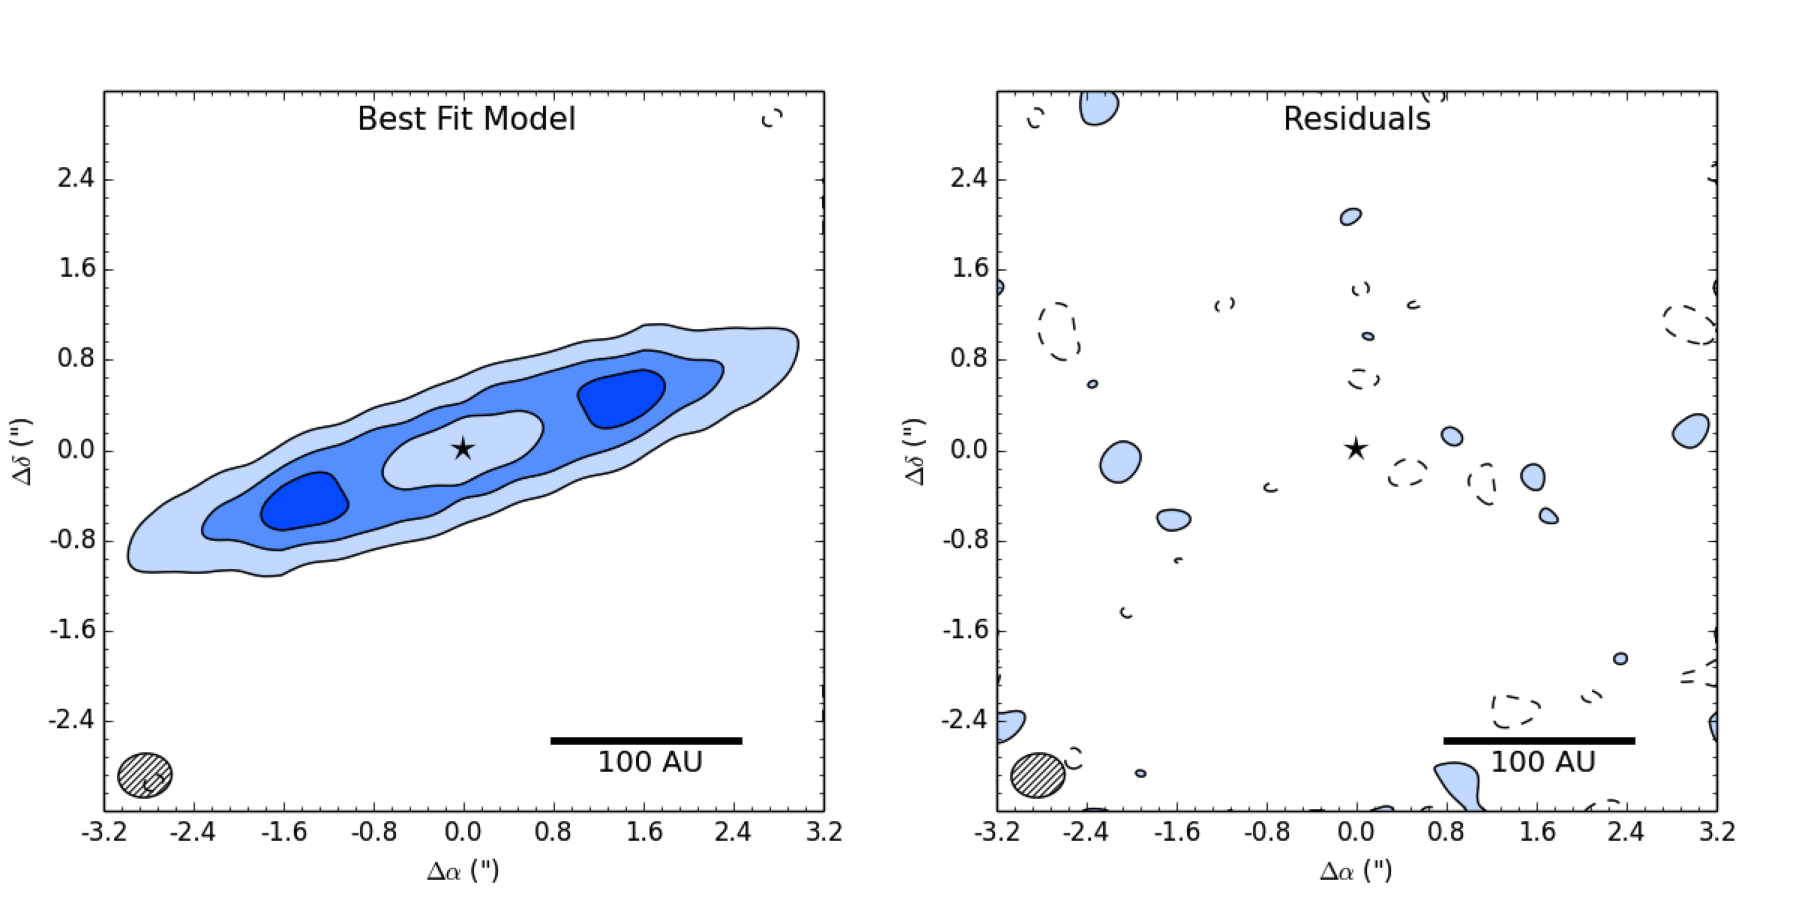
\includegraphics[width = 1\textwidth]{49CET_dPBAG_ModelResidual.png}
\caption{The model image (left) and residuals (right) for the double power law with an an additional inner disk of small grains. Contours are [-2, 2, 4, 6] $\times$ 58$\,\mu$Jy. The model leaves only a small scatter of 2$\sigma$ residuals.}
\label{fig:49CET_dPBAG_ModelResidual}
\end{figure}

\subsection{Simultaneous SED and Visibility Fit with Two Characteristic Grain Sizes}

As with the single power law model and the USDE model, we describe an inner disk of 0.1$\,\mu m$ grains extending from $R_{In}$ to $R_{Inner Disk}$ ($R_{In} + \Delta R_{Inner Disk}$) with $\Sigma_{Inner Disk} \propto r^{-1}$. We now vary $p_{1}$ from $R_{Inner Disk}$ to $R_{T}$ and vary $p_{2}$ from $R_{T}$ to $R_{Out}$, with $R_{T}$ = $R_{In} + \Delta R_{Inner Disk} + \Delta R_{T}$ and $R_{Out}$ = $R_{In} + \Delta R_{Inner Disk} + \Delta R_{T} + \Delta R_{Out}$. This model restores $p_{1}$ to the value derived from the visibility only fit within our uncertainties, and results in a model that isn't too bright at the center and doesn't leave behind positive residuals at $\sim$ 100\,AU. The best-fit model and residual images are shown in Figure \ref{fig:49CET_dPBAG_ModelResidual}, the SED is displayed in Figure \ref{fig:49CET_dPBAG_SED}, and the table of parameters is presented in Table \ref{tab:dPBAG_Table}.

\begin{figure}[t!]
\label{fig:49CET_DP_SED}
\centering
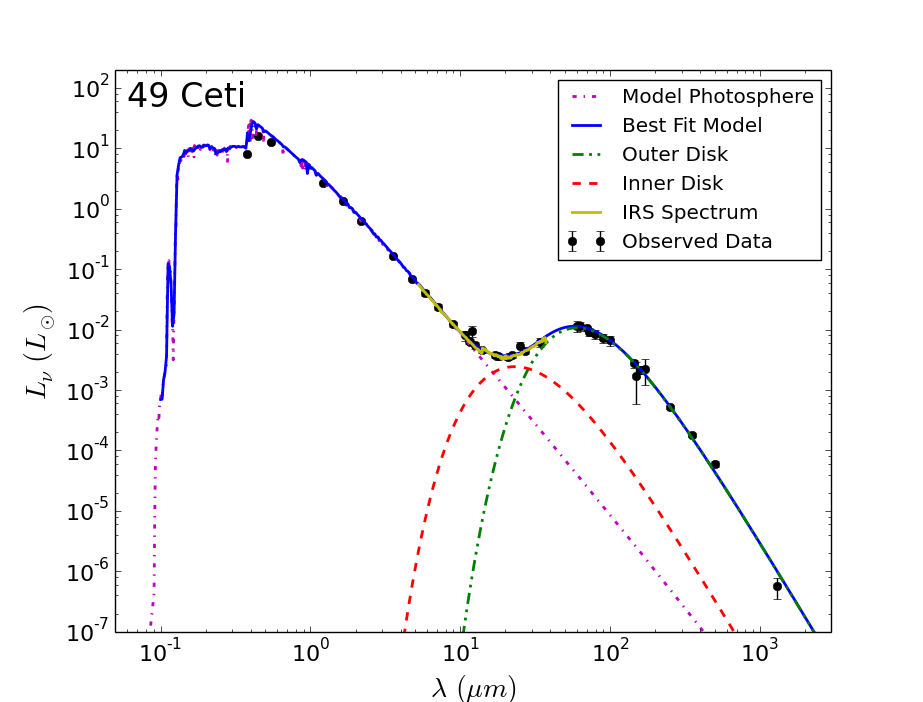
\includegraphics[width = 1\textwidth]{49CET_dPBAG_SED2.png}
\caption{The SED for the double power law model fitting the SED and visibilities for the two-part disk model. }
\label{fig:49CET_dPBAG_SED}
\end{figure}

\begin{table}[t!]
\begin{center}
    \def\arraystretch{1.37}%
    \begin{tabular}{l*{2}{c}r}
    \hline
    Parameter & Median Value $\pm$ 1$\sigma$ & Best Fit Value \\ \hline
     $R_{In}$  [AU] & 4.0$^{+1.3}_{-1.0}$ & 3.4\\  
     $\Delta R_{Inner Disk}$ [AU] & 45$^{+9}_{-11}$ & 37\\ 
     $\Delta R_{T}$ [AU] & 51$^{+12}_{-9}$ & 59\\ 
     $\Delta R_{Out}$  [AU] & 222$^{+11}_{-13}$ & 216\\ 
     log($M_{Inner Disk}$ [$M_{\oplus}$]) & -4.64$^{+0.15}_{-0.19}$ & -4.81 \\
     log($M_{Outer Disk}$ [$M_{\oplus}$]) & -1.76$^{+0.11}_{-0.11}$ &-1.72 \\
     log(a [$\mu$m]) & 0.08$^{+0.11}_{-0.12}$ & 0.10\\ 
     $\beta$ & 1.16$^{+0.06}_{-0.05}$ & 1.18\\ 
     $p_{1}$ & -1.9$^{+0.8}_{-1.4}$ & -2.0\\ 
     $p_{2}$ & 1.47$^{+0.15}_{-0.14}$ & 1.48\\ 
     $i$ [$^\circ$] & 79.3$^{+0.4}_{-0.4}$ & 79.2 \\ 
     $PA$ [$^\circ$] & -71.5$^{+0.4}_{-0.5}$ & -71.3\\
    \hline
    \end{tabular}
\end{center}
\caption{Values derived from the MCMC chain for the double-power law model with two characteristic grain sizes.}
\label{tab:dPBAG_Table}
\end{table}
%dPBAG 40x800 SED+VIS (correct sig fig) }

%%%%%

\section{Statistical Comparison of Best-fit Models}
\label{stats}

While the difference in residuals between the single power law, double power law, and USDE models for both the is not significant at any one location in the disk, these disparities may be statistically significant when considered over the whole ensemble of data and model visibilities. One method for getting a sense of whether there are any systematic errors in our models relative to the data involves deprojecting the visibilities. This radially averages them within elliptical annuli matching the disk inclination, which effectively increases the signal to noise ratio by $\sim$ 2$\pi$, although this factor also depends on the binning of our data. As can be seen in Figure \ref{fig:deprojected_DP_PL_Vis}, the best-fit visibility-only single power law model visibilities underestimate the data by a small but systematic amount between baseline lengths of $\sim$ 500 kilolambda and $\sim$ 600 kilolambda. These long baselines resolve some of the smallest angular scales, suggesting that the model might be missing some of the finer details of the disk. 

\begin{figure}
\centering
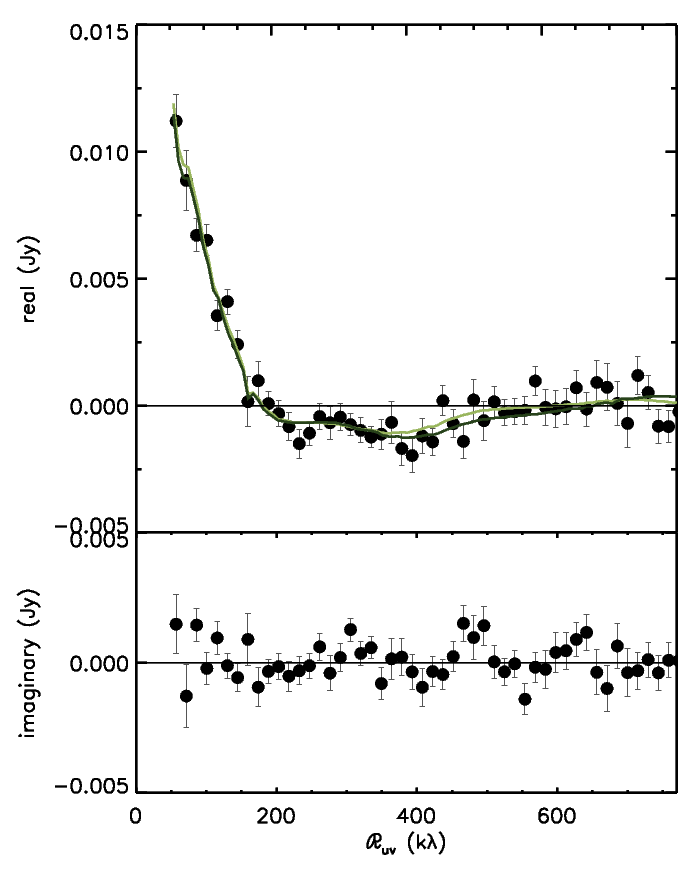
\includegraphics[width = 1\textwidth]{49CET_bestModelDeprojections_data_greenDP_blackPL.png}
\caption{The deprojected real and imaginary data visibilities are plotted in black with corresponding error bars. The green line displays the deprojected best-fit visibility-only double power law model visibilities, and the black line shows the deprojected best-fit visibility-only single power law model visibilities. A subtle but consistent systematic underestimation of the real visibilities between $\sim$ 500 kilolambda and $\sim$ 600 kilolambda is apparent for the single power law model.}
\label{fig:deprojected_DP_PL_Vis}
\end{figure}

In order to understand whether the differences between the model fits are statistically significant, we apply the Akaike Information Criterion (AIC) derived from information theory and the Bayesian Information Criterion (BIC) derived from Bayesian statistics as independent tests of whether one model is statistically better than another. A key assumption of both the AIC and BIC tests is that the posterior distribution functions are Gaussian or nearly Gaussian \citep{Lidd07}. All of our parameters from the MCMC chain are well constrained and fill out posterior distributions that fit this criteria, so we deem both tests applicable for our purposes. The AIC is defined as:

\begin{equation}
\label{eq:AIC}
\text{AIC} = -2\,\text{ln}\,\mathcal{L}_{\text{max}} + 2k
\end{equation}

where $\mathcal{L}_{\text{max}}$ is the maximum possible likelihood for the model in question (ie. the minimum $\chi^{2}$) and $k$ is the number of parameters in the model \citep{Akai74}. For $N$ data points, $\mathcal{L}_{\text{max}}$ is defined as:

\begin{equation}
\label{eq:fancyL}
\mathcal{L}_{\text{max}} = \prod_{i=1}^{N} \frac{e^{-\chi^{2}_{min}/2}}{\sqrt{2\pi} \sigma_{i}}
\end{equation} 

\begin{table}[t!]
\begin{center}
\def\arraystretch{1.37}%
\begin{tabular}{l*{3}{c}}
\hline
\hline
Model              & Single Power Law & USDE & Double Power Law  \\
\hline
$\chi^{2}_{Vis}$ & 141308.5 & 141289.617 & 141289.344   \\
%AIC            & -7.7174 & -3.7171 & -3.7171 \\
BIC           & 1689894.79 & 1689852.34 & 1689852.07 \\
%BIC           & 70.5706 & 94.1429 & 94.1429 \\ this is the top line wiki BIC val
\hline
\end{tabular}
\caption{$\chi^{2}_{Vis}$ for the single power law, USDE model, and double power law fitting just the visibilities. BIC values were calculated with Equation \ref{eq:BIC}.}
\end{center}
\label{tab:stats_table1}
\end{table}


%more easily manipulated as ln($\mathcal{L}_{\text{max}}$), which is defined as: 

%\begin{equation}
%\label{eq:fancylnL}
%\text{ln}\,\mathcal{L}_{\text{max}} =  \frac{-\chi^{2}_{min}}{2 \sqrt{2\pi}} \sum_{i=1}^{65700} \sqrt{w_{i}}
%\end{equation} 

Plugging Equation \ref{eq:fancyL} into Equation \ref{eq:AIC}, we find that the probability any differences are random between two models, $p$, is:

\begin{equation}
\label{eq:relLikelihood}
p = \text{exp}\bigg(\frac{AIC_{\text{a}}-AIC_{\text{b}}}{2}\bigg) =  \text{exp}\bigg(\frac{\chi^{2}_{min,\text{a}}-\chi^{2}_{min,\text{b}}}{2}\bigg + k_{a} - k_{b}\bigg)
\end{equation} 

%\begin{equation}
%\label{eq:relLikelihood2}
%p = \text{probability any differences are random} = \text{exp}\bigg(\frac{-\Delta \chi^{2}}{2}+\Delta \text{number of parameters}\bigg)
%\end{equation} 

%$\Delta \chi^{2}~\text{(Single Power Law With Ring vs. Double Power Law)} = 3.63 \\ p = 0.16 \approx 1\sigma$

%$\Delta \chi^{2}~\text{(Single Power Law With Ring vs. Single Power Law)} = 14.83 \\ p = 0.004 \approx 3\sigma$

%(1 $-$ prob) is the relative likelihood of model $a$ being better than model $b$. 

The BIC, first defined by \cite{Schw78_BIC}, is described as:

\begin{equation}
\label{eq:BIC}
%\text{BIC} = -2\,\text{ln}\,\mathcal{L}_{\text{max}} + k\,\text{ln}\,N
\text{BIC} = \chi^{2} + df\,\text{ln}\,N
\end{equation}

where $\chi^{2}$ is the minimum chi-squared, df is the number of degrees of freedom, and $N$ is the number of data points. If $\Delta$BIC (ie. BIC$_{a}$ - BIC_{b}$) between two models is $>$ 10, the evidence is very strong that model $b$ is better than model $a$ \citep{Kass95}. 


\begin{table}
\begin{center}
\def\arraystretch{1.37}%
\begin{tabular}{l*{3}{c}}
\hline
\hline
Model              & Single Power Law & USDE & Double Power Law  \\
\hline
 $\chi^{2}_{Vis}+$\chi^{2}_{SED}$ & 141322.080 & 141307.250 & 141310.861   \\
%AIC            & -3.7176 & 0.2826 & 0.2826 \\
BIC           & 1689884.80 & 1689846.40 & 1689850.01\\
%BIC           & 94.1424 & 117.7146 & 117.7146\\ top line wiki BIC val
\hline
\end{tabular}
\caption{$\chi^{2}_{Vis}+$\chi^{2}_{SED}$ for the single power law, USDE model, and double power law models with two characteristic grain sizes. BIC values were calculated with Equation \ref{eq:BIC}.}
\end{center}
\label{tab:stats_table2}
\end{table}

The AIC returns the same result for the USDE model and the double power law model for just the visibility fit as well as the two-part disk model, and $\Delta$BIC between these two models is less than 5 in each case, suggesting that they are statistically indistinguishable. From Equation \ref{eq:relLikelihood}, we find that the models with a surface density enhancement at $\sim$ 110\,AU are are significantly better than the single power law models at the $\sim 4\sigma$ level for the visibility-only fits and at the $\sim 3\sigma$ level for the two-part disk models. Complementing this result, $\Delta$BIC $\sim$ 40 for comparing both the USDE and double power law to the single power law, so with a high degree of confidence, we posit that the models of the surface density with peak values at r $\sim$ 110\,AU best represent the physical nature of 49 Ceti's dust disk. 

%For the visibility-only fits, Equation \ref{eq:relLikelihood} shows that the both the USDE and double power law models are better than the single power law model at the $\sim$ 4$\sigma$ level (will calculate exact value later), and that there is no statistical difference between USDE and double power law models.  

%are truer to the physical 
%0.135 times as likely as the single power law to ``minimize the information loss" for both the visibility-only and two-part best-fit models.  $<<$ what does this really mean tho??? 

From a philosophical standpoint, further evidence for the significance of the density enhancement at $\sim$ 110\,AU comes from the fact that both of our more complex models could have effectively ignored the additional parameters---the USDE model could have prescribed $M_{Ring}$ = 0 and had its values for the power law and transition radius match those of the best-fit single power law model, and the double power law model could have settled on two decreasing power laws such that the surface density for the outer disk would match that of the single power law---but they didn't. Rather, within our derived uncertainties, they ascribe the peak of the surface density to be at the same radius (Figure \ref{fig:densityDistr}). Even though it seems in this plot that the turnover from inner disk to outer disk for the single power law is close to the radius of the peak density, it settles on $R_{Inner Disk}$ = 73 $\pm$ 3\,AU, significantly smaller than the peak surface density at a radius of 114$^{+3}_{-3}$\,AU and 100$^{+15}_{-14}$\,AU for the USDE and double power law models, respectively. 

%$\sim$ 110AU in the double power and USDE models. 

\begin{figure}
\centering
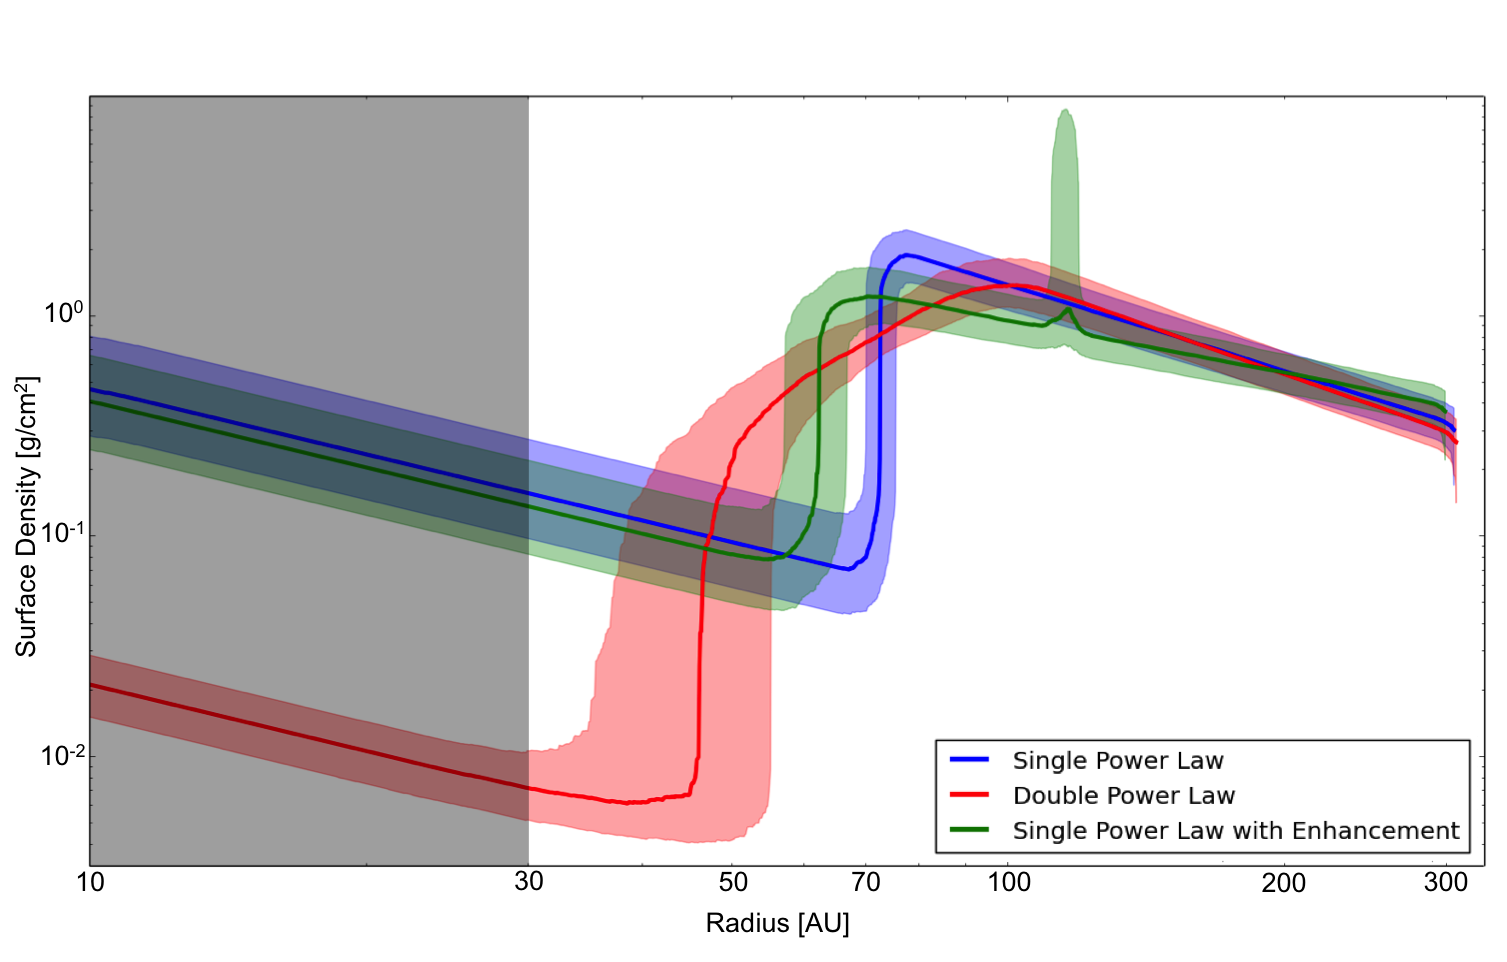
\includegraphics[width = 1\textwidth]{49CET_SDD2_withShaded_oldPerson.png}
\caption{The best-fit surface density distributions for the single power law, USDE, and double power law models with two characteristic grain sizes are shown as thick lines, with their uncertainties ($\pm$ 1$\sigma$) displayed as the respective shaded color. The grey shaded region denotes the spatial resolution of our ALMA data, helping to exhibit that the surface density distribution is not well characterized for the inner disk, where $\Sigma_{\text{Inner Disk}} \propto r^{-1}$ by definition and the scaling is only affected by the fit to the SED.}
\label{fig:densityDistr}
\end{figure}

%See Tables \ref{tab:49CET_nOBAG_Table}, \ref{tab:bBBAG_Table}, and \ref{tab:dPBAG_Table} for exact values related to the plotted parameters.


%e^-chi2/2 / root2pi(product of square root of weights)

%flux is spread around imaging
%radial averaging improves SNR by 2pi
%see that plot systematics
%at small scales

%clean does weird things to noise in images
%noise in vis isn't equal to noise in iamge
%don't understand how noise transfers through clean process



%%%%%%

%Transition radius = transition radius
%outer radius = inner radius + delta rOut



%%%%


\section{Mid-Infrared Properties}
\label{MidIR}

\begin{figure}[t!]
\centering
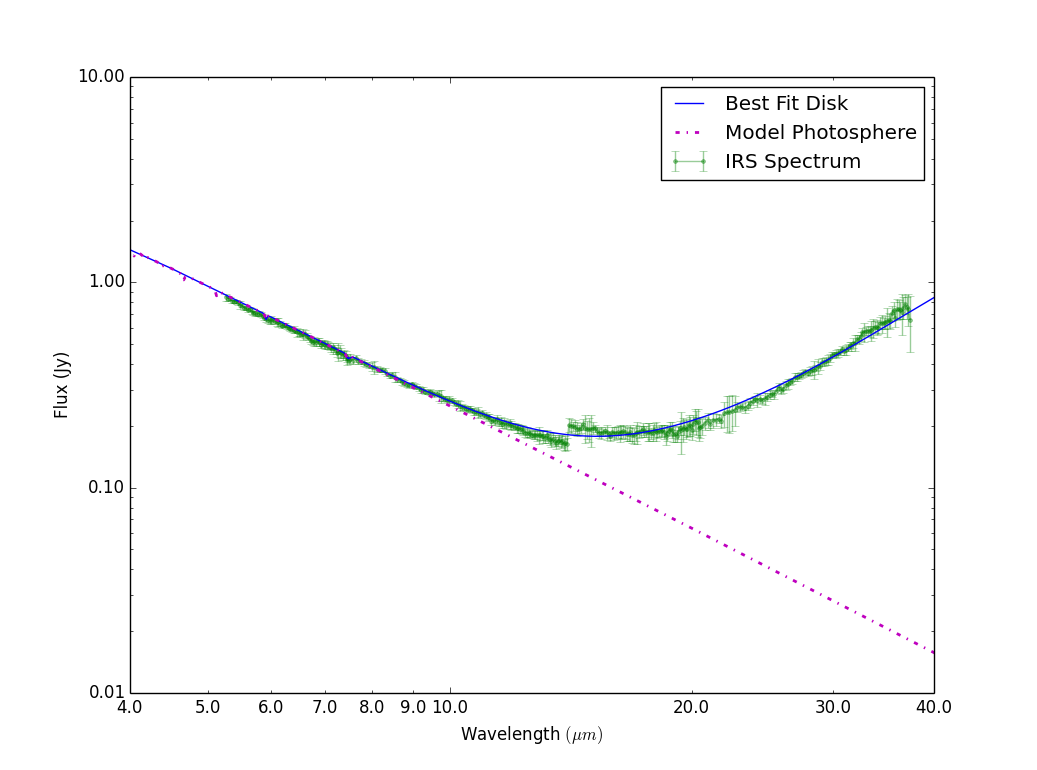
\includegraphics[width = 1\textwidth]{49CET_IRS_Window.png}
\caption{The IRS spectrum of 49 Ceti is plotted in green along with each point's statistical uncertainty. The absolute calibration uncertainty used in fitting the SED, assumed to be 10$\%$ of the flux measurement, is not displayed. A sample best-fit disk and the model photosphere are plotted for reference.}
\label{fig:49CET_IRS_Window}
\end{figure}


The detail and accuracy of the 360 points that make up the $\it{Spitzer}$ IRS spectrum, presented in Figure \ref{fig:49CET_IRS_Window}, allow us to see characteristic emission features of silicate grains (or the lack thereof). The jump at 14$\,\mu m$ in the spectrum is not an emission feature, but rather a calibration issue resulting from the fact there are two separate sub-modules being used to take spectra within IRS (one from 5 - 14$\,\mu m$, the other from 14 - 40$\,\mu m$). We do not see any emission features at 10$\,\mu m$, where emission due to silicate grains usually peaks, but the implications of this absence of silicate emission is so far unclear due to insufficient observational constraints. 

Silicate features are most apparent when the emitting grains are smaller than $\sim$ 1$\,\mu m$ \citep{Papo83}, but  \cite{Natt07} show that 10$\,\mu m$ spectral features are also apparent in the emission of 200-600K grains smaller than a few microns. Our best fit models suggest an inner radius of $\sim$ 5\,AU, which is right on the border of where we expect to find grains at this temperature,  so it might be that there simply aren't grains with the right properties to display any mid-IR features. 

% but can be washed out if they are not the dominant emitters. 
%In addition, even if there are grains of this size, if the crystal lattice structure is uneven, the emission feature will be less pronounced. \cite{Natt07} suggest that the 10$\,\mu m$ spectral region probes 200-600K grains smaller than a few microns confined to the disk surface within $\sim$ 10AU of the star for protoplanetary disks and within $\sim$ 1AU from the star in the case of T Tauri stars. Our best fit model suggests an inner radius of ?????, which is right on the border of where we expect to find these grains with these characteristics, so it might be that there simply aren't grains with the right properties to display any mid-IR features. 

It is possible that the percentage of silicate grains is low in 49 Ceti's disk, and that the composition of the grains is dominated by carbon. The high albedo of silicate grains is usually responsible for reflecting enough light to be seen in scattered light imaging, but the non-detection of the disk at separations $>$ 1.6 arcsec \citep{Wein99} in scattered light provides evidence that silicates may not dominate the composition. In addition, \cite{Robe14} find an extreme carbon overabundance relative to iron, suggesting that the disk is volatile-rich. However, $\beta$ Pic shows the same overabundance of carbon, but it is easily seen in scattered light with \textit{HST}. 

%Because silicates tend to have much higher albedos than carbon-based grains, the non-detection of any scattered light at separations $>$1.6$''$ \ref{Wein99} suggests that 
%All of these are possibilities for 49 Ceti's disk, but it is unclear what the dominant reason is that we do not observe any silicate features. 



\chapter{Discussion}
\label{Discussion}

\section{Dust Disk Characteristics and Stirring Mechanisms}

49 Ceti's unique dust disk and its substantial reservoir of molecular gas given its age are special features that help illuminate the late stages of disk evolution. Its broad dust disk displays a population of small, $\sim$ 0.1\,$\mu m$ grains that extends from $\sim$ 4 to $\sim$ 60\,AU, and a population of larger, $\sim$ 1.6\,$\mu m$ grains that extends from $\sim$ 60 to $\sim$ 300\,AU. The surface density of the dust peaks at $\sim$ 110\,AU, suggesting a region of enhanced collisions between planetesimals. Preliminary analysis of the CO emission suggests that a substantial mass of CO is co-located with the dust, indicating that similar processes may be shaping their morphologies. 

\subsection{Self-Stirring}
\label{SelfStirring}

Replenishment of mm-sized grains through destructive collisions of planetesimals requires impact velocities that can only be achieved in a dynamically stirred environment \citep{Moor13}. Self-stirring scenarios, in which $\sim$ 1000\,km planetesimals destabilize smaller bodies into eccentric orbits, can produce the velocities necessary to produce significant amounts of dust \citep{Keny04}. In the resulting collisional cascade, which propagates from the inside out due to the larger densities and velocities of material closer to the star, the highest concentration of dust is produced near the largest parent body. \cite{Keny08} described the timescale for the formation of the first 1000\,km object as: %100-300m$\,$s$^{-1}$ is what Keny04 said but meh

\begin{equation}
\label{eq:t1000km}
t \approx 145~x_{m}^{-1.15}\bigg(\frac{a}{80\text{AU}}\bigg)^{3}\bigg(\frac{2M_{\odot}}{M_{\bigstar}}\bigg)^{\sfrac{3}{2}} ~~[\text{Myr}]
\end{equation}

where $a$ is the semi-major axis of a dust belt, $M_{\odot}$ is the solar mass, $M_{\bigstar}$ is the mass of the central star being considered, and $x_{m}$ is a scaling factor in describing the initial surface density, $\Sigma_{i}$:

\begin{equation}
\label{eq:MMSNsurf}
\Sigma_{i}(a) = \Sigma_{0}(M_{\bigstar})~x_{m}~\bigg(\frac{a}{a_{0}}\bigg)^{\sfrac{-3}{2}}~~~[\text{g}~\text{cm}^{-2}]
\end{equation}

A sensible reference surface density for $x_{m}$ to scale is that of the minimum mass solar nebula (MMSN), for which $\Sigma_{0} \approx 0.18$\,g\,cm$^{-2}$ at $a_{0}$ = 30\,AU \citep{Weid77}. The MMSN is the minimum mass of material required to form the solar system, scaled to solar composition. \citeauthor{Keny08} assume this surface density scales linearly with the mass of the central star, such that:

\begin{equation}
\label{eq:massMMSNscale}
\Sigma_{30\text{AU}}(M_{\bigstar}) \approx 0.18 \bigg(\frac{M_{\bigstar}}{M_{\odot}}\bigg)~~~[\text{g}~\text{cm}^{-2}]
\end{equation}

We can solve for the scaling factor $x_{m}$ from Equation \ref{eq:t1000km}:

\begin{equation}
x_{m} \approx 145^{\sfrac{1}{1.15}}~\bigg[t \bigg(\frac{a}{80\text{AU}}\bigg)^{-3}\bigg(\frac{2M_{\odot}}{M_{\bigstar}}\bigg)^{\sfrac{-3}{2}}~\bigg]^{\sfrac{-1}{1.15}}
\end{equation}

With t = 40 (in units of Myr), $a$ = 110\,AU, and $M_{\bigstar}$ = 2.0\,$M_{\odot}$, $x_{m} \approx$ 8. In other words, the minimum mass necessary produce a dense ring at 110\,AU by 40\,Myr with self-stirring processes is roughly 8 times the ``minimum mass 49 Ceti nebula," which is twice as massive as the MMSN (as per Equation \ref{eq:massMMSNscale}). With a gas-to-dust ratio of 100:1, as is canonical for protoplanetary disks, \cite{Must09} found that $x_{m}$ must be less than 10, as values of $x_{m}$ $>$ 10 resulted in discs that were gravitationally unstable at $>$ 100\,AU. 49 Ceti's high-density ring at $>$ 100\,AU and $x_{m}$ $<$ 10 suggest that the disk is gravitationally stable and self-stirring is a viable means for producing the level of collisions necessary to sustain the density enhancement that peaks at $\sim$ 110\,AU.  

\subsection{Planetary Stirring}
\label{PlanetStirring}

The gravitational influence of a giant planet is another means of stirring planetesimals in the disk to destructive collisional velocities. Eccentricity and semi-major axis of the planet's orbit ($e_{pl}$ and $a_{pl}$), the stellar mass, ($M_{\bigstar}$), and the required excitation velocity for destructive impacts between bodies ($v_{rel}$) all have an impact on the maximum spatial extent over which a giant planet has the influence to initialize catastrophic collisions. For micron-sized silicate grains, $v_{rel}$ must be above 1 m$\,$s$^{-1}$ in order to exceed the ``sticking" threshold \citep{Gutt10}. In the outer disk, where weak conglomerations of ices dominate, \cite{Must09} describe $v_{rel}$ as a function of particle radius ($R$):

\begin{equation}
\label{eq:grainV}
v_{rel}(R) = \Bigg[0.8\bigg(\frac{R}{80\text{m}}\bigg)^{-0.33} + 0.8\bigg(\frac{R}{80\text{m}}\bigg)^{1.2}\Bigg]^{0.83}~~[\text{m s}^{-1}]
\end{equation}

This function has a minimum of 1 m$\,$s$^{-1}$ for bodies $\sim$ 80m in radius and suggests that impact velocities of tens of meters per second are necessary for destructive collisions between micron-sized ices. Destructive collisions between grains of $R\sim$ 1-10cm easily produce the $100\mu m$-1mm particles that dominate the emission at the wavelength of our ALMA image. This is the size that grains achieve by sticking before they tend to break each other apart (the famous ``meter size barrier" problem, see \citealt{Blum08}). However, it is also worth considering km-sized comets, as collisions between bodies of this size produce a variety of observable grains and meter-sized bodies, which in increase the rate of collisions. Both grains between $R\sim$ 1-10cm and km-sized bodies need collisional velocities of 5-10 m$\,$s$^{-1}$ to result in destructive collisions. For an internal perturber, the semi-major axis ($a^{\ast}$) within which a giant planet can excite grains of radius $R$ to $v_{rel}$ is given by \cite{Must09} as:

\begin{equation}
a^{\ast}(R) = 3.8 \bigg(\frac{e_{pl}}{0.1}\bigg)^{\sfrac{2}{3}} \bigg(\frac{M_{\bigstar}}{1M_{\odot}}\bigg)^{\sfrac{1}{3}} \bigg(\frac{a_{pl}}{1\text{AU}}\bigg)^{\sfrac{2}{3}} \bigg(\frac{v_{rel}(R)}{1\text{km s}^{-1}}\bigg)^{\sfrac{-2}{3}}~~[\text{AU}]
\end{equation}

Using the characteristics of Jupiter's orbit as a reference, ie. $e_{pl}~\sim$ 0.05 and $a_{pl}~\sim$ 5.2\,AU, along with 49 Ceti's mass (2\,$M_{\odot}$), we find that destructive collisions for cm-sized grains ($v_{rel} \sim$ 5-10 m$\,$s$^{-1}$, Equation \ref{eq:grainV}) can be triggered out to $\sim$ 200-300\,AU, well beyond the orbit of 49 Ceti's ring. 

This distance is irrespective of the planet's mass, but the timescale over which the effect takes place depends both on the planet's mass and semimajor axis. This timescale can be modeled as:

\begin{equation}
\label{eq:planetExciteTime}
t \sim 1.53 \times 10^{3} \frac{(1-e_{pl}^{2})^{\sfrac{3}{2}}}{e_{pl}}\bigg(\frac{a}{10\text{AU}}\bigg)^{\sfrac{9}{2}} \bigg(\frac{M_{\bigstar}}{1M_{\odot}}\bigg)^{\sfrac{1}{2}} \bigg(\frac{M_{pl}}{1M_{\odot}}\bigg)^{-1} \bigg(\frac{a_{pl}}{1\text{AU}}\bigg)^{-3}~~[\text{yr}]
\end{equation}

\begin{figure}
        \makebox[\textwidth][c]{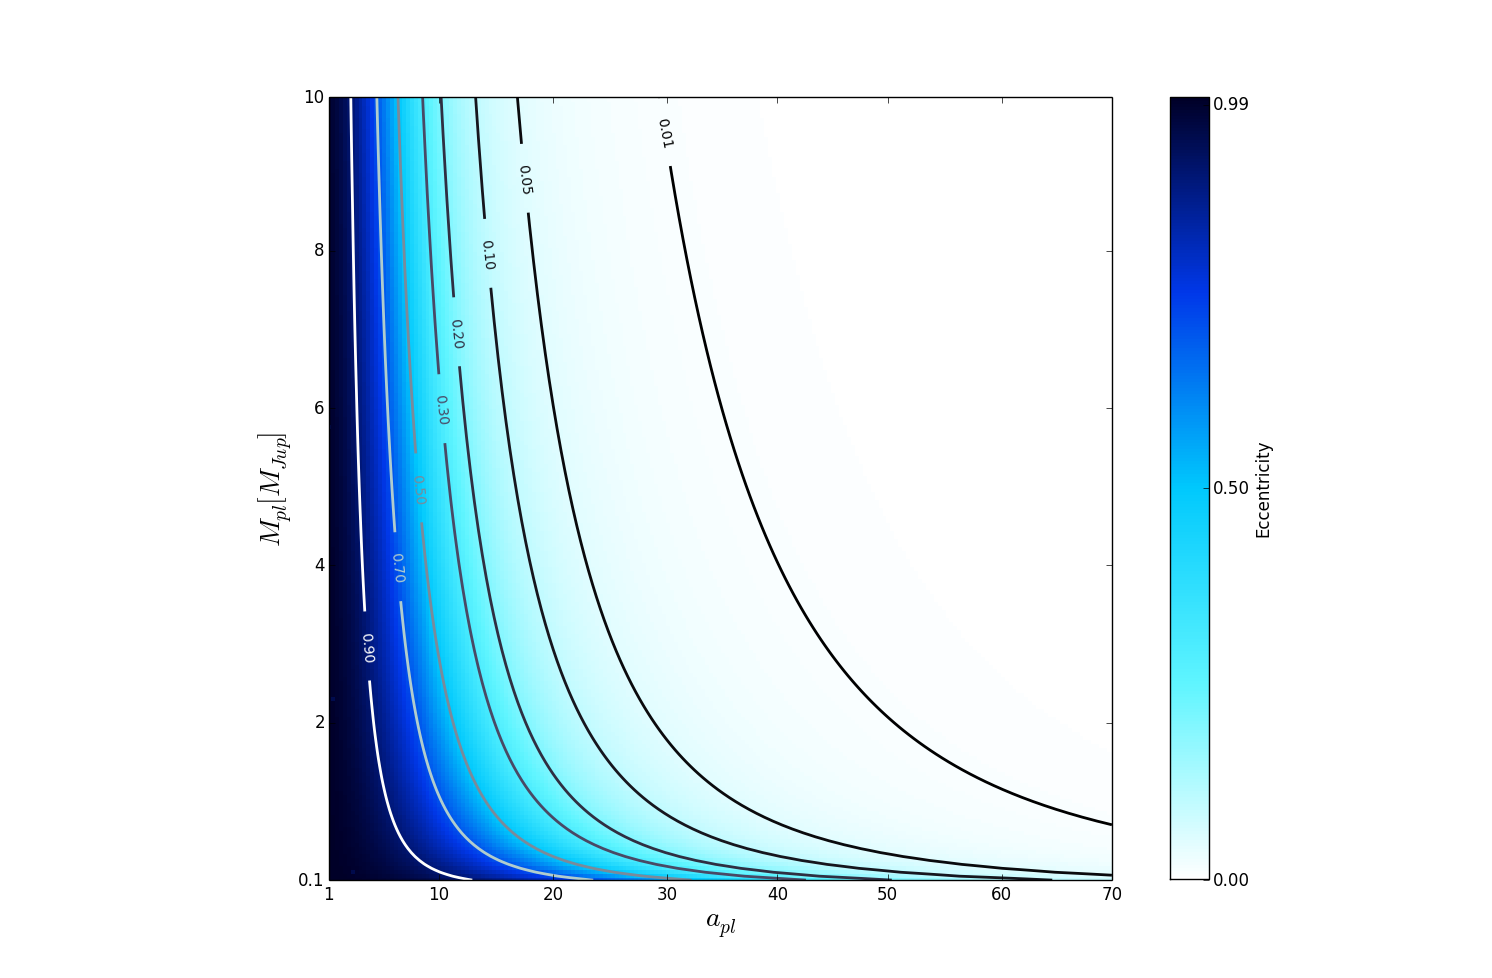
\includegraphics[width=1.6\textwidth]{49CET_stirPlot_Good_newaxes3.png}}%
	\caption{The eccentricity in $a_{pl}$, $M_{pl}$ parameter space needed to stir the planetesimal belt at $\sim$ 110\,AU in less than 49 Ceti's age of 40\,Myr. The contour lines correspond to $e_{pl}$ = 0.01, 0.05, 0.10, 0.20, 0.30, 0.50, 0.70, and 0.90.}
	\label{fig:49CET_StirringPlot}
\end{figure}

%Using Jupiter's orbital characteristics from earlier, and its mass, $M_{pl} \approx 10^{-3} M_{\odot}$, we find that the timescale for perturbing planetesimals at 110AU is on the order of 10 billion years. 

Figure \ref{fig:49CET_StirringPlot} displays the eccentricity required for a planet of semi-major axis $a_{pl}$ and mass $M_{pl}$ to stir the planetesimal belt at 110\,AU in less than 49 Ceti's age of 40\,Myr. A Jupiter-like planet, with $e_{pl}~\sim$ 0.05, $a_{pl}~\sim$ 5.2\,AU, and $M_{pl} \approx 10^{-3} M_{\odot}$, can not be responsible for stirring the ring. However, if this planet were at $a_{pl}~\sim$ 40\,AU (holding $e_{pl}$ and $M_{pl}$ constant), it would be able to excite planetesimals to collisional velocities in less than the age of the system. 

%Equation \ref{eq:planetExciteTime} is very sensitive to the eccentricity of the given planet, so 

%More realistic timescale estimates come easily from increasing the eccentricity, 

%are highly sensitive to the eccentricity. 

%Excluding the time that it takes to actually form this reference planet, 

%a more realistic timescale estimate of roughly 40Myr for the stirring of 49 Ceti's planetesimal ring is obtained if this Jupiter mass planet were at a separation of $a_{pl}$ = 40\,AU (holding everything else constant). 

%Another realistic situation is that of a 10$M_{Jup}$ planet at $a_{pl}$ = 20\,AU, which would also have a stirring timescale of $\sim$ 40Myr for the ring.

Both planetary-stirring and self-stirring are viable options for maintaining the level of collisions necessary to sustain 49 Ceti's planetesimal ring. \cite{Must09} suggest that there is a radius beyond which the disc will stir itself before a giant planet can stir it, and describe this radius as:

\begin{equation}
\label{eq:planetvself}
\Phi \sim 630~x_{m}^{-0.77} (1-e_{pl}^{2})^{-1}e_{pl}^{\sfrac{2}{3}}\bigg(\frac{a_{pl}}{1\text{AU}}\bigg)^{2}  \bigg(\frac{M_{pl}}{1M_{\odot}}\bigg)^{\sfrac{2}{3}} \bigg(\frac{M_{\bigstar}}{1M_{\odot}}\bigg)^{\sfrac{-4}{3}}~~[\text{AU}]
\end{equation}

From the opposite perspective, if a dust ring exists within the value given by Equation \ref{eq:planetvself}, it must be planet-stirred. As we showed earlier, $x_{m} \gtrsim 8$ for self-stirring to have acted out to 110\,AU within 40\,Myr. This is the one case for which 49 Ceti's planetesimal ring is self-stirred, assuming any Jupiter-like planets are within $\sim$ 40\,AU. If a planet with Jupiter's orbital characteristics exists at any separation larger than $\sim$ 40\,AU, $\Phi > 115$\,AU (holding $x_{m}$ at 8), implying that planet-stirring would be responsible for the dust ring. 

While having 8 times the ``minimum mass 49 Ceti nebula" is certainly possible, it isn't very likely. \cite{Andr13} find observationally that the median mass ratio of a protoplanetary disk to its host star is $\sim$ 0.3$\%$, that the upper quartile has $\sfrac{M_{disk}}{M_{\bigstar}} \geq 1\%$, and that only a handful have $\sfrac{M_{disk}}{M_{\bigstar}} \geq 10\%$. The MMSN is 0.013\,$M_{\odot}$\citep{Desc07}, so 49 Ceti's minimum mass nebula would have a mass of 0.026\,$M_{\odot}$. 8 times this mass gives $\sfrac{M_{disk}}{M_{\bigstar}} = 10.4\%$, which puts it just on the edge of possibility. 

If the initial mass of 49 Ceti's protoplanetary disk were closer to the median suggested by \citeauthor{Andr13}, ie. $M_{disk} = 0.006\,M_{\odot}$ and $x_{m} \sim$ 0.25, there are still many plausible scenarios in which planets are responsible for exciting planetesimals in the ring. In order for a planet to stir the ring in less time than the age of the system, it must be at a separation of at least 40\,AU from the star (with $e_{pl}~\sim$ 0.05 and $M_{pl} \approx 10^{-3}\,M_{\odot}$, as earlier) as per Equation \ref{eq:planetExciteTime}. Even if $x_{m} <$ 0.25, planetary stirring can still be responsible for stirring the ring in a timescale less than the age of the system, as $x_{m}$ affects the timeline for self-stirring but not the timeline for planet stirring. $x_m$ likely has a significant influence on the timescale for giant planet formation, but this connection is not well established and is only starting to be probed with observations. 

%Based on this analysis, it is more likely that a planet between 1-10$M_{Jup}$ at a separation greater than 40AU (for the 1$M_{Jup}$ planet) or 20 AU (for the 10$M_{Jup}$ case) is responsible for stirring the planetesimal ring. These planets need to coalesce quickly enough such that their gravitational impact on the ring occurs in less time than the combined age of their formation and timescale of influence, so it is probable that the previous estimates of mass and semi-major axis for a perturbing planet are on the low end, as these hypothetical planets would take the full 40Myr of 49 Ceti's lifetime to stir the ring. 

For example, recent evidence of planet formation in the 1-2\,Myr old HL Tau system \citep{Part15} suggests these processes may happen much more quickly than in the canonical outlook, which says that giant planets must form within $\sim$ 10\,Myr of stellar formation \citep{Poll96}. Estimates of the dust mass in HL Tau's disk range between 0.03-0.14\,$M_{\odot}$ \citep{Robi07}, which relative to its stellar mass of 0.7\,$M_{\odot}$ \citep{Clos97} suggest $x_{m} \gtrsim$ 3-16 (remember $x_{m}$ = 1 corresponds to when $M_{disk}$ = 0.013\,$M_{\bigstar}$). HL Tau's disk displays ring-like structure in alternating light and dark bands out to $\sim$ 100\,AU, with the spectral index of the darker rings suggesting significant grain growth. Large planets have probably coalesced and are responsible for shaping these gaps in the disk.

%a series of light and dark rings at wavelengths between 870$\mu m$ and 2900$\mu m$, %With such a massive protoplanetary disk, it is apparent that planet forming processes occur rapidly. 

HL Tau shows us that large values of $x_{m}$ leads to planet formation processes out to $\sim$ 100\,AU in short timescales, providing additional circumstantial evidence that 49 Ceti's ring may be planet stirred. If $x_{m}$ were large enough such that self-stirring could be viable, it is likely that giant planets would form beyond a critical $a_{pl}$ that sets the critical radius $\Phi$ for which a ring would be planet stirred or self stirred for a given $x_{m}$ (Equation \ref{eq:planetvself}). If $x_{m}$ = 8 (the minimum for a self-stirring scenario for 49 Ceti's ring), it is logical, as per observations of HL Tau, that giant planets would be forming throughout the disk in only a few Myr. In this situation, any planet slightly more massive, closer, or more eccentric than that suggested by Figure \ref{fig:49CET_StirringPlot} (as to leave a few Myr for planet formation) would be responsible for the stirring. 
%Leaving a few Myr for formation of the planet, any planet with a suitable combination of $M_{pl}$, $a_{pl}$, and $e_{pl}$ as described by Figure \ref{fig:49CET_StirringPlot} would 
%Based on the timescales for planetary stirring suggested by Equation \ref{eq:planetExciteTime} and the critical radius from Equation \ref{eq:planetvself}, planets slightly larger or closer than the 10$M_{Jup}$ planet at 20AU and 1$M_{Jup}$ planet at 40AU (larger or closer such that stirring timescales would be shorter, leaving a few Myr for formation) would be responsible for the stirring. 

If the planetary stirring scenario is indeed the correct one, this has significant implications for planet formation. \cite{Must09} posit that the largest planetesimal that an interior planet can destroy at a separation $a$ is given by:

\begin{equation}
\label{eq:planetDestruction}
R_{max} \approx 74 \bigg(\frac{e_{pl}}{0.1}\bigg) \bigg(\frac{M_{\bigstar}}{M_{\odot}}\bigg)^{\sfrac{1}{2}} \bigg(\frac{a}{10\text{AU}}\bigg)^{\sfrac{-3}{2}} \bigg(\frac{a_{pl}}{1\text{AU}}\bigg)~~[\text{km}]
\end{equation}

The 1\,$M_{Jup}$ planet at 40\,AU considered earlier would be able to destroy planetesimals up to radii of $\sim$ 50\,km at 110\,AU and $\sim$ 200\,km at 50\,AU. This suggests that growth of planetesimals beyond this barrier would become extremely difficult after the aforementioned planet coalesced. Even if bodies larger than this existed prior to the this planet's formation, the resulting increase in the velocity dispersion from the Jupiter-mass planet would impede growth rates. This suggests that multiple planet systems form simultaneously, as there are significant disturbances in the disk after large planets have formed. 

%Note that Equation \ref{eq:planetDestruction} is not dependent on the mass of the planet, but rather is linear with respect to the planet's eccentricity and semi-major axis. 

\subsection{Broad Dust Disk Component}

From our modeling, we find that 49 Ceti's outer disk beyond the surface density enhancement at $\sim$ 110\,AU is well described by a decreasing power law, with $\Sigma \propto r^{-0.8}$ for the USDE model and $\Sigma \propto r^{-1.5}$ for the double power law. The standard point of comparison for disks is the surface density of the MMSN \citep{Weid77,Haya81}, which is found to fall off as $r^{-1.5}$ (see Equation \ref{eq:MMSNsurf}). However, this assumes that the planets of the Solar System formed in situ. If the planets have undergone significant radial migration, which is certainly possible \citep{Levi03}, the inferred density profile for the MMSN could be significantly distorted from the true initial conditions. Observations of 24 circumstellar disks in the $\sim$ 1\,Myr old Ophiuchus-Scorpius and Taurus-Auriga star forming region find that $\Sigma \propto r^{-1}$ after the removal of systematic effects \citep{Andr07}, and subsequent analysis of the nine brightest protoplanetary disks in Ophiuchus corroborate this result, finding that the median initial surface density falls off as $r^{-0.9}$ \citep{Andr09}.  

In 40 million years of evolution, however, it is logical to expect that the processes shaping the disk should have altered it significantly from initial conditions. Steady accretion disks, with $\alpha$ constant and the viscosity proportional to the radius, have $\Sigma \propto r^{-1}$ \citep{Shak73,Hart98}. In addition, simple mass conservation arguments for a disk where radiation pressure driven outflows dominate show that the surface density should fall off as $r^{-1}$, which matches the profile of Vega's debris disk \citep{Su05}. 

Rings of increased collisions of planetesimals, which generate a large diversity of grain sizes, can have a distinct impact on the morphology of the rest of the disk. One such ``birth ring," in AU Mic, acts as the divider between an inner disk of millimeter-sized grains and an outer disk of micron-sized grains. \cite{Stru06} suggest that the small grains migrate outwards due to radiation pressure, whereas large grains fall inward due to corpuscular and Poynting-Robertson (CPR) drag. Further, they show that the outer disk is collision-dominated, as the population of small grains falls off as $r^{-3/2}$, matching theory. 

The hypotheses put forth to explain the distribution of grains in the case of Vega and AU Mic only describe the expected surface density profile of micron-sized grains and do not touch on the processes that shape millimeter-sized grains in debris disks. It is tempting to extend the theories that describe the small grains to larger grains, but the morphology of micron-sized grains can be different from the larger grains traced by our observations. Using conjectures for the processes that shaped these disks to describe 49 Ceti's disk, which seems to show the opposite arrangement of small and large grains, would be unwise. Although collisions, radiation pressure, and CPR drag certainly play a role in sculpting 49 Ceti's dust disk, the presence of gas complicates how these mechanisms act. More theoretical modeling is needed before we will be able to understand the processes responsible for different surface density profiles of millimeter grains.  

%The evolution of debris disks, whether gas-poor or gas-rich, is not well understood, 


%However, this argument considers grains just above the blowout size (i.e. $\sim$ 10$\mu m$), and the morphology of these grains can be different than the larger grains traced by our observations. 


%, and that this power law describes the scattered light images of AU Mic well. 



%find AU Mic's outer disk of small grains is collision-dominated, as it lined up with predictions showing that small grains should fall off as $r^{-3/2}$ in this case. 

%In collision-dominated disks, the outer population of small grains should fall off as $r^{-3/2}$ \citep{Stru06}, and this is four to 

%This phenomenon is observed in AU Mic, where grains of all sizes are created in one of these rings $\sim$ 40AU from the star. 

%Beyond this ring, only micron-sized grains are observed, whereas millimeter-sized grains are seen in the inner disk \citep{Macg13}. The surface density distribution of the outer disk is sensitive to what processes dominate. If corpuscular and Poynting-Robertson drag dominate, the distribution of micron sized grains should fall off as $r^{-5/2}$, whereas the population of grains in collision-dominated disks falls off as $r^{-3/2}$ \citep{Stru06}. 

% due to processes that act differently on each grain population. 


%$In addition, certain accretion disk collapse scenarios predict $\Sigma \propro r^{-1}$ \citep{Shak73}. 

%http://iopscience.iop.org/0004-637X/632/1/670/pdf/62699.web.pdf

%, with relatively gentle power law slope, 

%-0.8pm0.2 for bBBAG
%-1.3pm0.1 for nOBAG
%-1.5pm0.2 for dPBAG


\section{Gas Disk Characteristics}

\begin{figure}
\centering
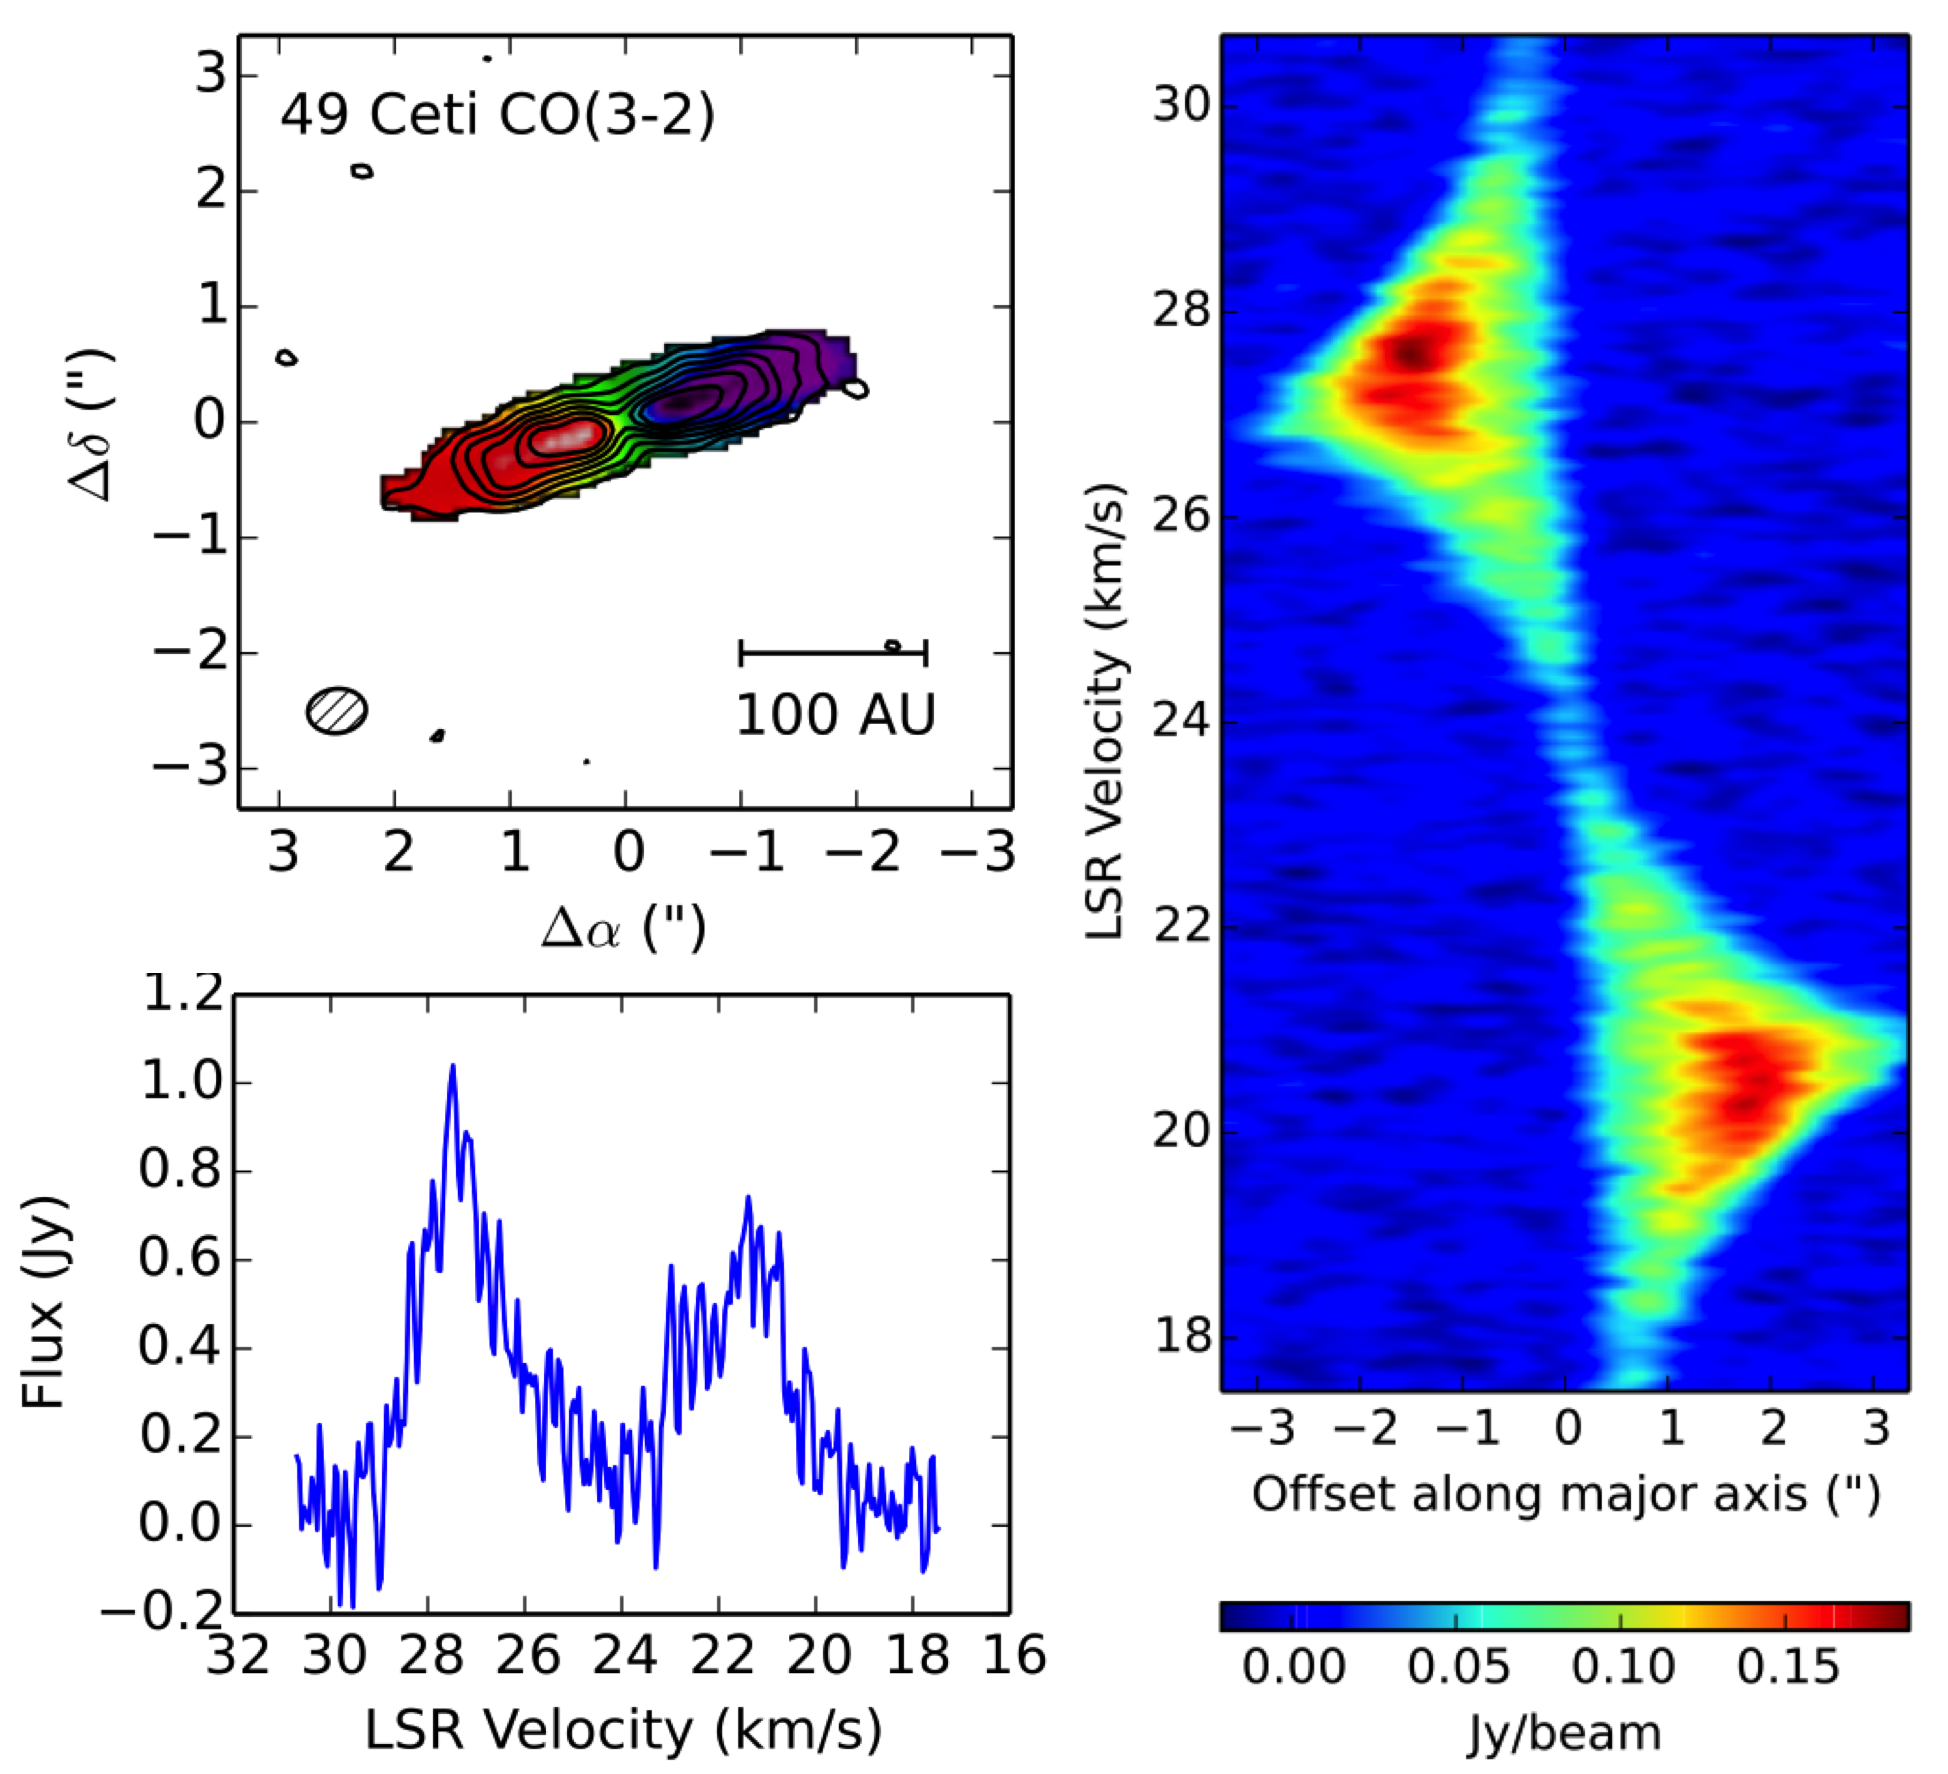
\includegraphics[width=\textwidth,height=\textheight,keepaspectratio]{49CET_CO_plots_sideby.png}
\caption{The zeroth (contours) and first (colors) moment maps are displayed in the top left panel. The contours are [3, 6, 9, 12, 15, 18] $\times$ 0.02 Jy beam$^{-1}$. The CO(3-2) spectrum is shown in the bottom left. The line exhibits a double-peaked structure that is characteristic of an inclined disk in Keplerian rotation about the central star. The southeast side of the disk is $\sim 40 \%$ brighter in integrated emission than the northwest side. A position-velocity diagram of CO(3-2) emission from the gas disk is presented in the right panel. The x-axis represents offset position from the southeast limb to the northwest limb along the disk major axis relative to the star position.}
\label{fig:49CET_CO_plots}
\end{figure}

Modeling of the CO detected around 49 Ceti at the J=3-2 transition has been inconclusive thus far. However, examination of the zeroth moment map and position-velocity (PV) diagram (see Figure \ref{fig:49CET_CO_plots}) reveals basic characteristics of the gas morphology. A separation of 1.43 $\pm$ 0.03 arcsec exists between the two peaks apparent in the zeroth moment map, corresponding to a separation of 87\,AU. This, in combination with the lack of a central peak and the relatively faint line emission indicating that the gas is optically thin, suggests that the inner disk is gas-poor within 44\,AU. This value is probably underestimated, however, as the beam detects flux from the front and back of the disk along the minor axis due to the disk's high inclination. This inner radius is consistent with the value of $\sim$ 90\,AU derived from CO(2-1) observations performed \cite{Hugh08} with the SMA. At its maximum along the major axis, 3$\sigma$ emission extends 7.3 $\pm$ 0.1 arcsec, which suggests the outer radius of the gas disk is $\sim$ 220\,AU. 

Preliminary models of the gas disk indicate $\sim 7 \times 10^{-7} M_{\odot}$ of CO (assuming a CO/H$_{2}$ abundance of 10$^{-4}$), and seem to show an increase in the density of gas at $\sim$ 100\,AU. The peak of nearly 0.20\,Jy\,beam$^{-1}$ in the PV diagram on the southeast side of the disk is separated by $\sim$ 1.6'' ($\sim$ 100\,AU) from the star's position, corroborating the results of those early models. While it appears that the southeast side of the disk is brighter in the spectrum and the PV diagram, this difference is not significant. 

\section{Gas in Debris Disks}

49 Ceti's three part dust disk, consisting of an inner disk of small grains and a broad outer disk of larger grains punctuated by a surface density enhancement, is unlike all other debris disk that have been studied in this level of detail. This, in combination with its significant mass of gas given its age, make it truly unique. However, there are a handful of other systems that seem like siblings to 49 Ceti---they are clearly all related, but none of them look quite the same. 

The gas we observe in other gas-rich debris disks can be primordial, left over from the formation of the star, or secondary, released through collisions of planetesimals. Protoplanetary disks are good at nursing large masses of gas due to effective shielding from the optically thick dust content \citep{Wyat14}, but as the dust disperses, the rate of photodissociation of gas accelerates, and most disks are found to be gas-poor by an age of 10\,Myr \citep{Zuck95}. In systems that display co-located gas and dust, the gas is assumed to be continually replenished by the same collisional mechanisms responsible for sustaining the secondary dust content, but in systems that display distinct gas and dust disks, another explanation is needed for explaining the presence of gas. Assuming the composition of comets and other icy bodies in exoplanetary systems is similar to that in the solar system, i.e. $\sim$ 10$\%$ CO by mass, maintaining the gas disk requires a hearty but not unreasonably large diet of volatile-rich dust, planetesimals, and comets. 

\subsection{ALMA-Resolved Gaseous Debris Disks}

In addition to 49 Ceti, the only gas-rich debris disks to be imaged in both gas and dust emission with ALMA are $\beta$ Pic and HD 21997. These systems provide a timeline for us to examine the processes that are shaping the gas and dust at this late stage of disk evolution. However, each displays distinct characteristics, exemplifying that this picture is not a simple one.

$\beta$ Pic, an A star, hosts a gaseous debris disk viewed edge-on that is very similar to 49 Ceti's. At only 19\,pc away, it was one of the first of its kind to be discovered and has been studied extensively both with resolved millimeter observations (with the SMA by \citealt{Wiln11}, ALMA by \citealt{Dent14}) and in coronographic scattered light imaging (first by \citealt{Smit84}, with STIS by \citealt{Heap00}, more recently by \citealt{Ahmi09}, \citealt{Mill14}, and \citealt{Apai15}). Its disk has a dust mass of $\sim 8\times10^{-2}$ $M_{\oplus}$ and $\sim 4\times10^{-5}$\,$M_{\oplus}$ of CO \citep{Dent14} at an age of $\sim$ 20\,Myr \citep{Bink14}. The millimeter dust probed by ALMA is distributed in an azimuthally asymmetric belt that is nearly co-located with sub-microns grains that have been revealed in scattered light imaging. The surface brightness peaks at 60\,AU from the star, nearly matching the inner radius of the gas disk, which extends from 50 to 160\,AU, peaking at 85\,AU. The CO dissociation timescale in $\beta$ Pic's outer disk is on the order of 100 years because of ionizing interstellar radiation, so CO is either continually replenished or we are observing the system $<$ 100 years after a significant collision. \cite{Moor15} found that given $\beta$ Pic's outer radius, a planet-stirring scenario is probably responsible for spurring collisions within the disk. 

%$12^{+8}_{-4}$ Myr \citep{Zuck01}.

%The birth ring at $\sim$ 40AU is likely creating grains of all sizes that are subject to different 

%reveal strong forward scattering and polarization out to $\sim$ 80AU, and the specifics arounhinting that the birth ring is made of highly porous ($\sim 90 \%$) primordial ices that formed beyond the frost line \citep{Grah07}. 

%resolved by SMA \citep{Wiln12}
%ACS on HST -- first polarization maps!! find that grains must be highly porous ($\sim90\%$)... possibly primordial because the birth ring lies beyond ice sublimation point \citep{Grah07}
%scattered light by \citep{Kala04}, \citep{Kris05}

The 30\,Myr old A star HD 21997, 72\,pc away, also hosts a gaseous debris disk. The dust disk extends from 55 to 150\,AU with the surface density decreasing as $\sim r^{-1.6}$ and has a mass of $\sim 9\times10^{-2}$\,$M_{\oplus}$ \citep{Moor13}. An estimated $\sim 6\times10^{-2}$\,$M_{\oplus}$ of CO extends from $\sim 25$\,AU to  $\sim 140$\,AU \citep{Kosp13}. The dust and gas seem to be co-located between 55 and 140\,AU, but within 55\,AU is a dust-poor inner region. 

The distinct locations of the dust and gas populations hint that different processes may be shaping their morphologies. \cite{Kosp13} suggest that the CO is primordial and has endured since the formation of the star due to very efficient shielding mechanisms, as maintaining the observed mass of CO through collisions of planetesimals and comets would require an unreasonably high gas production rate of 10$^{19}$\,kg\,yr$^{-1}$ ($\sim 10^{-6}\,M_{\odot}$\,yr$^{-1}$). However, \cite{Moor13} posit that the dust is secondary, as models by \cite{Kriv09} state that the lifetime of grains in a gaseous debris disk with a gas-to-dust ratio of 100 is less than 2 $\times$ 10^{4} years. As with $\beta$ Pic, HD 21997's disk is probably planet stirred, as its outer radius is greater than a 10 minimum mass stellar nebula could self-stir to within 30\,Myr \citep{Moor15}. If correct, the primordial gas scenario implies efficient radial drift of grains due to strong gas-dust coupling, which hints that the extended dust disk could be the result of efficient migration from a narrow, planet-stirred planetesimal ring. 

HD 141569, an A star $\sim$ 110\,pc away that is 5\,Myr old, displays CO emission in addition to displaying the qualities of a debris disk, but the gas disk has not yet been resolved with any millimeter interferometer. Scattered light imaging by \cite{Wein00} reveals that the disk extends out to $\sim$ 360\,AU with a gap in the disk at $\sim$ 250\,AU. Gaps like these are suggestive of continual clearing and secondary dust production processes. \cite{Brit07} find that the gas emission comes from within $\sim$ 40\,AU of the star, but it is unclear if the dust traces the gas, as the scattered light imaging is only able to see micron-sized grains at greater than $\sim$ 70\,AU and millimeter observations have not been performed. 
%This extreme pace, equivalent to the complete destruction of $\sim$ 6000 Hale-Bopp sized comets each year, argues against the secondary replenishment scenario, unless we are observing HD 21997

%HD 21997's disk has not been detected in scattered light by recent \textit{HST} observations \citep{Kris10}, implying a low albedo for the grain population. However, this non-detection could also result from the disk falling below the sensitivity limit of the ACS coronagraph due to the distance of the system. 

\section{Debris Disks Resolved by ALMA}

The resolution and sensitivity now available with ALMA in examining continuum emission from circumstellar material is helping detail how secondary dust is created and the processes that shape its morphology. Often, the dust is produced in a ``birth ring," which has an enhanced region of collisions relative to other parts of the disk. The handiwork of planets can appear as distinct structures of the surface density. Clearing by a planet can result in a distinct gap in the dust disk, whereas a narrow ring with abrupt cutoffs suggests gravitational interaction with one or more planets.

%The of this birth ring has implications for the timescale since stirring began, as the spread of grains in opposite directions by forces that work differently on small and large grains. 

The M-type star AU Mic, part of the $\beta$ Pic moving group at an age of $\sim$ 20\,Myr, hosts an edge-on debris disk that displays no CO emission. As with $\beta$ Pic, its proximity to Earth (10\,pc) has made it a popular target for observation. Millimeter observations with the SMA by \cite{Wiln12} and with ALMA by \cite{Macg13} find that the dust disk increases steeply in surface density ($\Sigma \propto r^{2.3}$) from $\sim$ 10-40\,AU before abruptly dropping off. This profile can be explained by a self-stirred disk with ongoing planet formation \citep{Kenn10}, but the timescale required to initiate the collisional cascade is much longer than its age (as per Equation \ref{eq:t1000km}, \citealt{Keny08}). Thus, planetary stirring is the likely cause of the peak in surface density at $\sim$ 40\,AU. Scattered light imaging detects the disk out to $\sim$ 210\,AU \citep{Kala04,Kris05}, and models of polarization maps of the disk indicate micron-sized grains extend from $\sim$ 40\,AU to $\sim$ 150\,AU \citep{Grah07}. \cite{Stru06} suggest that a birth ring exists at $\sim$ 40\,AU in which grains of all sizes are created through collisions. The smaller grains, highly susceptible to stellar winds and radiation pressure, are blown out on highly eccentric orbits, whereas larger grains fall inward due to CPR drag. 

The 100\,Myr G-type star HD 107146 and its gas-poor disk give a snapshot of the very late stages of debris disk evolution. At 28\,pc, it has been resolved at millimeter wavelengths with CARMA \citep{Cord09} and the SMA \citep{Hugh11}, but recent Cycle 0 observations with ALMA are able to ascertain more detailed structure \citep{Ricc15}. The ALMA continuum data detect emission from 30-150\,AU that can be equivalently modeled by a double power-law for the surface density that decreases to $\sim$ 70\,AU before increasing thereafter and by a shallowly increasing single power-law with a $\sim$ 8\,AU gap at $\sim$ 80\,AU. The simplest explanation for the clearing in the dust disk is that a planet of a few $M_{\oplus}$ has coalesced and cleared a nearly circular orbit at $\sim$ 80\,AU. The increasing surface density in the outer disk can be explained by a self-stirring scenario, but only if $x_{m} \geq 10$, which is unlikely but not impossible (see Section \ref{SelfStirring}). 

Optical and near-IR scattered light imaging of HD 107146 revealed micron sized grains extending from $\sim$ 50 to $\sim$ 230\,AU, with a peak in density at $\sim$ 130\,AU \citep{Ardi04,Erte11}. Like in $\beta$ Pic, where micron-sized grains are not co-located with their larger brethren, the two grain populations in HD 107146 show distinctly different morphologies. This isn't necessarily unsurprising, as grains in HD 107146's disk have been subject to the physical mechanisms of CPR drag and radiation pressure that act more efficiently on small grains for longer timescales. 

At $\sim$ 440\,Myr old and only $\sim$ 8\,pc away, the debris ring around the A star Fomalhaut is one of the oldest that has been thoroughly studied. Early efforts to observe the ring at millimeter wavelengths \citep{Holl98,Ricc12} detected the ring but lacked the resolution to accurately trace the emitting grain population (and thus the parent body morphology). However, more recent ALMA observations resolve the eccentric ring and find it is $\sim$ 15\,AU wide with sharp inner and outer boundaries, has a semi-major axis of $\sim$ 140\,AU, and has an eccentricity of $\sim$ 0.1 \citep{Bole12}. These observations are in agreement with scattered light imaging by \cite{Kala05} that showed a peak brightness in scattered optical light at the same distance. The morphology of the ring suggests that it is confined by gravitational interaction with one or more planets \citep{Chia09}.

\section{49 Ceti in Context}

49 Ceti is a rare example of a gas-rich debris disk, displaying properties not observed in protoplanetary disks. The broad dust disk characterized by two grain sizes underlying the enhancement at $\sim$ 110\,AU is a unique morphology that hasn't been observed in other systems. Although the inner disk doesn't necessarily fill out all the way to $R_{Inner Disk}$ (this was an assumption in modeling following the approach of \citealt{Wahh07}), there is a clear transition at this radius where an outer disk of larger grains begins. The mechanisms responsible for distinct populations of small ($\sim 0.1 \mu m$) grains in the inner disk and larger ($\sim 1.6 \mu m$) grains in the outer disk is not well understood given our data. We hypothesize that the dust in 49 Ceti's planetesimal ring at $\sim$ 110\,AU is continually replenished and that it is probably stirred by an interior planet (Section \ref{PlanetStirring}). 

\begin{figure}
	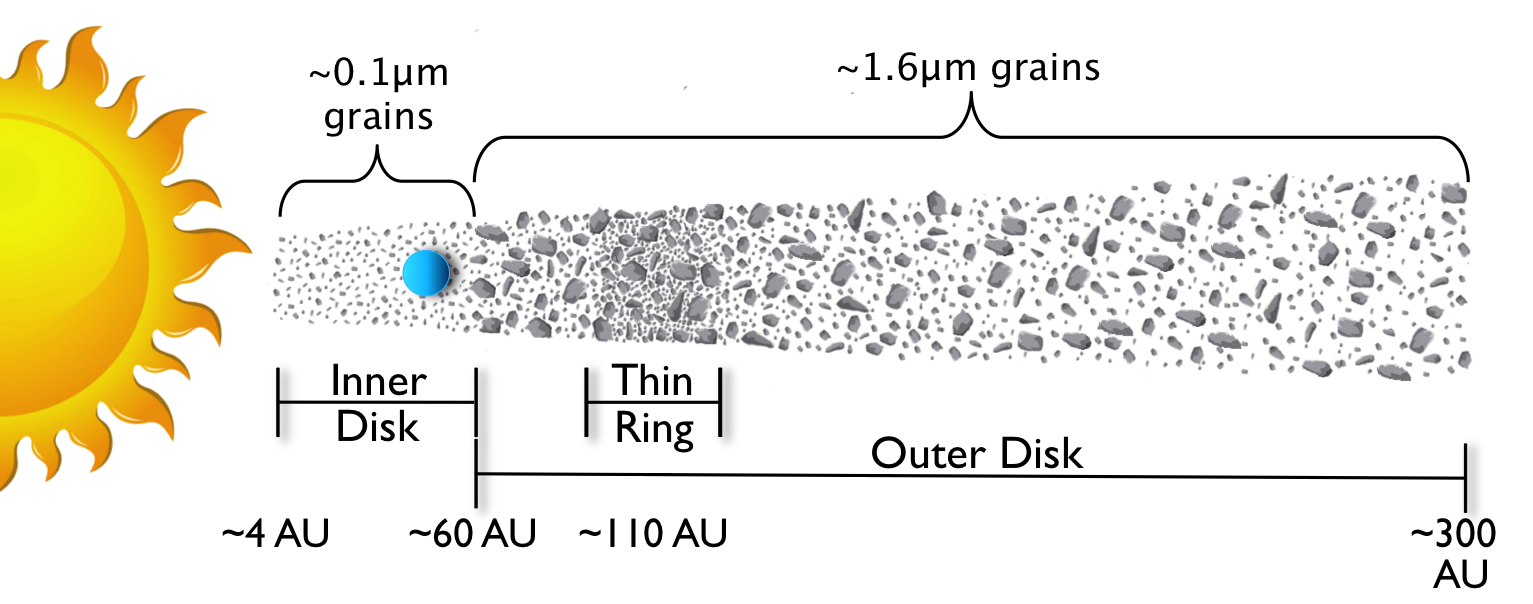
\includegraphics[width = 1\textwidth]{49CET_DustDistributionCartoon2_ForThesis.png}
	\caption{A cartoon of the dust distribution of 49 Ceti. The enhancement in the surface density is shown as a narrow ring here (the USDE model, see Section \ref{USDE}), but it can be equivalently described by a double power law that peaks at this radius (see Section \ref{DP}). We find that planetary stirring is responsible for promoting collisions in this planetesimal belt, but our data are unable to constrain the location or mass of this planet.}
	\label{fig:49CET_DDC}
\end{figure}

The diversity of debris structures that have been previously observed exemplify how complex disk evolution is and 49 Ceti only adds to this intricate picture. The sharply increasing surface density structure of AU Mic is consistent with predictions for self-stirring, but the 1000-km planetesimals at the peak density of the ring necessary for this scenario could not have in the age of the system, suggesting planetary stirring may be responsible. However, no gaps in the surface density distribution suggestive of planets, such as the one in HD 107146, are observed in AU Mic. Fomalhaut's ring seems more typical of older debris systems that have had more time to evolve. Of the gas-rich debris disks, HD 21997 shows a dust disk with a steeply decreasing power law for the surface density that doesn't seem to be co-spatial with the gas disk, whereas $\beta$ Pic's gas and dust disks are effectively co-located. 49 Ceti's dust disk, with a peak in the surface density on top of a broad decreasing component, doesn't resemble any of the debris disks with no gas or HD 21997, but it's disk is quite similar to $\beta$ Pic's disk.
%; additionally it helps to limit the number of parameters needed to recreate the data

Preliminary analysis puts a strong lower limit for the inner edge of the 49 Ceti's gas disk at 44\,AU and suggests a peak in the density at $\sim$ 100\,AU, which corresponds closely with the geometry of the outer dust disk. This co-location of material signifies that secondary processes are almost certainly responsible for producing the gas and dust we observe at this late stage of disk evolution. $\beta$ Pic displays essentially this same structure, although the distribution of small grains is slightly different in these two systems. For 49 Ceti, small grains are limited to an inner disk that extends roughly $\sim$ 60\,AU from the star \citep{Wahh07}, whereas in $\beta$ Pic, small grains permeate through the entirety of the outer disk of millimeter grains as resolved by ALMA \citep{Apai15}. In addition, 49 Ceti displays no brightness asymmetry in CO or dust emission, though $\beta$ Pic does. As asymmetries in debris rings can arise easily from 2:1 mean-motion resonances with inner planets, this suggests the birth ring of $\beta$ Pic may be at roughly twice the radius of an unseen interior planet of $>10~M_{\oplus}$ \citep{Dent14}. The lack of an asymmetry in 49 Ceti's planetesimal belt could mean that the giant planet responsible for stirring isn't in resonance with the ring, or that our observations aren't high enough sensitivity to detect any asymmetry.






%T%his morphology, as is true in $\beta$ Pic as well, suggests 
%This may signify that similar processes are shaping the gas and dust disks at this late stage of disk evolution. As the ages of 49 Ceti, $\beta$ Pic, and HD 21997 are older than the timescale during which gas and dust generally disperse and few efficient shielding mechanisms are apparent, it is likely that the dust and CO that we observe is second-generation, produced through collisions of planetesimals and icy bodies. 

%, this would mean 49 Ceti is similar to $\beta$ Pic. This likely asymmetry raises the possibility of a $>10~M_{\oplus}$ planet in the outer disk that shepherds the dust and gas in a mean-motion resonance, increasing the likelihood of collisions at a specific radius, as may be the case in $\beta$ Pic (Dent et al.\ 2014). This would help explain how such a significant mass of co-located CO and sub-mm dust continue to be visible as 49 Ceti ages. 


%Generally it is expected that disks with actively stirred planetesimal rings have similar morphologies (optical vs mm), as collisional processes produce grains of all sizes that emit or reflect light from the optical out to millimeter wavelengths
%long wavelength images trace best the location and distribution of larger colliding bodies as the small grains probed at optical and near IR wavelengths react strongly to stellar radiation and wind forces... large grains in mm emission have dynamics like parent planetesimals (not my words) \citep{WYATT2006 IF YOU USE THIS, see sec. 6 of 107146 paper}. 

%CO is not detected, suggesting that the primordial gas has dispersed or coalesced into large bodies and that it is not being replenished. 


%The typical size of bodies in the disk affects how efficient a planet can be at promoting grinding collisions. For bodies $\sim$ 80m in size, a planet can stir the disk out to a radius given by: 
%\begin{equation}
%a = 1800\text{AU} e_{pl}^{\sfrac{2}{3}} \bigg(\frac{M_{\bigstar}}{1M_{\odot}}\bigg)^{\sfrac{1}{3}} \bigg(\frac{a_{pl}}{1\text{AU}}\bigg)^{\sfrac{2}{3}}
%\end{equation}

%MARS SIZED COLLISION???!?
%rare. talk beta pic and its asymmetry. 



%Observations at sub-millimeter wavelengths trace emission from large, $>100\mu m$ grains. Gas free-- little affected by radiative forces-- gas weak-- only weak coupling between gas and dust (TAKEUCHI & ARTYMOWICZ 2001). 

%comets sublimate at 110K (Wyatt 2008, the textbook one), so contribution of cometary gas to disk must be through collisions to be released


 %and as gas and dust lifetimes are very short 

%The co-location of gas and dust indicates that similar processes may be 


%either due to a mean-motion resonance with a giant planet or from the recent collision of mars-sized bodies

\chapter{Summary and Conclusions}

We resolved 49 Ceti's outer disk in both continuum emission and CO for the first time using ALMA Cycle 1 observations at a wavelength of 850\,$\mu m$. To investigate the geometry of the dust disk and the size distribution of its constituent grains,  simultaneously modeled the ALMA visibilities and unresolved fluxes from the SED with three axisymmetric functional forms of the surface density: 1) a single power law, 2) a single power law with a narrow, spatially unresolved belt, and 3) a double power law. We found that all of these models were unable to recreate the data unless an inner belt with a smaller characteristic grain size was introduced. With this two-part disk model, we found that the inner disk, characterized by small, $\sim$ 0.1\,$\mu m$ grains, extends from $\sim$ 4 to $\sim$ 60\,AU, and that larger, $\sim$ 1.6\,$\mu m$ grains populate the outer disk, which extends from $\sim$ 60 to $\sim$ 300\,AU. 

The two-part disk models that account for a peak in the surface density distribution, i.e. the single power law with the spatially unresolved belt and the double power law, better reproduce the ALMA data than the single power law. These two models, which peak at 114$^{+3}_{-3}$\,AU and 100$^{+15}_{-14}$\,AU, respectively, are indistinguishable within our uncertainties. This suggests that the enhancement in the surface density is unresolved by our data, which have a resolution of $\sim$ 30\,AU. The peak in surface density suggests a region of enhanced collisions between planetesimals. \cite{Moor15} were the first to suggest that planetary stirring was responsible for the extent of the dust disk as derived from Herschel images ($\sim$ 250\,AU), but the density enhancement discovered in this work provides a better tracer for the radius at which active stirring takes place. Using the radius of this newfound ring, our analysis confirms this result. While we are unable to see the responsible planet directly, its signature is apparent in promoting planetesimal collisions and creating the millimeter-sized dust that we observe. 

%This ring is almost certainly stirred by the gravitational influence of an interior giant planet. T

There is a substantial mass of gas co-located with the millimeter-sized dust due to collisions between volatile-rich bodies and planetesimals. This secondary material is likely continually replenished in order to maintain the mass of dust and CO that we detect. The processes responsible for the distinct inner disk of small grains are not well understood, though breakup and sublimation of comets play a role \citep{Wahh07}. There is a disparity between the submicron-sized grains suggested for the inner disk by \citeauthor{Wahh07} and the lack spectral features in the IRS spectrum, one that can potentially be resolved if 49 Ceti's disk is dominated by carbonaceous grains rather than silicates. New scattered light observations with \textit{HST}/ACS will likely act as the tiebreaker here, as previous coronagraphic imaging may have failed to detect the disk simply due to sensitivity limitations and the distance of 49 Ceti rather than the low albedo of the grains. However, if future observations with \textit{HST}/ACS do not display any reflected dust, 49 Ceti's dust disk would be the lowest albedo system ever measured. 

% co-location of a substantial mass of CO with the millimeter-sized dust indicates collisions of volatile-rich bodies and planetesimals are responsible for maintaining the mass of the disk. If 

The unique morphology of 49 Ceti's dust disk and its substantial reservoir of molecular gas given its age are special features that help illuminate the late stages of disk evolution. Our ALMA data were able to resolve the outer dust disk at millimeter wavelengths for the first time, providing the means with which to trace the distribution and dynamics of the parent planetesimal belts. However, subtleties in the surface density distribution could have been washed out by our beam. For example, we can not tell the difference between the narrow ring and double power law descriptions of the surface density. In addition, we were unable to resolve the morphology of the inner disk, which could provide tantalizing clues to the location and mass of a possible planet. Future observations, with higher sensitivity and resolution, may be able to resolve these nuances. In addition, if the planet is at the separations we expect and maximum elongation, direct imaging is within the realm of possibility. While we have written a new chapter in understanding 49 Ceti and its implications for the evolution of circumstellar material, it is by no means a closed case. Advanced observations will almost certainly reveal new and exciting clues about the processes of planet formation.


\medskip
\bigskip\bigskip
\bigskip
This work was partially supported by NSF grant AST-1412647. This paper makes use of the following ALMA data: ADS/JAO.ALMA\#2012.1.00195.5. This research has made use of the SIMBAD database, operated at CDS, Strasbourg, France, and of NASA's Astrophysics Data System. 




%-----------------------------------------------------------------------------------------------------------------------------------------
%% APPENDIX

%tell LaTeX that you're now in the appendix section:

\appendix

%I wanted my title formatting to be slightly different here, so that things are numbered "Appendix A" instead of "Chapter A" or "Chapter 6"

\titleformat{\chapter}{\bf\huge}
{Appendix \thechapter}{-5.35em}{\\}
\titlespacing*{\chapter}{0pt}{-.5in}{*3}


%These are the file names of my appendices:
%\chapter{Distance Calculations}
\label{distcode}

%\chapter{Spectral Absorption and Emission}
\label{specbackground}

%
\chapter{The Nature of LINERs}
\label{LINERs}


\doublespacing


%-----------------------------------------------------------------------------------------------------------------------------------------
%%BIBLIOGRAPHY:

\fancypagestyle{plain}{%
% clear all header and footer fields, we don't want these for the bibliography
\fancyhf{} 
% except we want the page number to sbhow up in the center of the footer:
\fancyfoot[C]{\thepage} 

\renewcommand{\headrulewidth}{0pt}
\renewcommand{\footrulewidth}{0pt}}
\pagestyle{plain}

%change title spacing once again, for the bibliography:
\titlespacing*{\chapter}{0pt}{-.75in}{*3}

%Add the bibliography to the table of contents, it doesn't show up by default, you have to specify it:
\addcontentsline{toc}{chapter}{\textbf {Bibliography}}

%The default for BibTex (the bibliography builder in LaTeX) is to not include citations that are in your bibliography file, but that you don't cite anywhere in the paper.  This changes that setting, so that all papers show up in the bibliography, whether or not you referenced them:
\nocite{*}

%Insert the bibliography (in this case, my file name was also "bibliography" if not, your line would read: \bibliography{my_workscited_filename} or whatever:
\bibliographystyle{apj}
\bibliography{bibliography}

%the end!
\end{document} 